\documentclass[11pt, twoside]{article}

\usepackage[]{geometry}

\usepackage{
	amsmath,
  	amssymb,
  	amsthm,
  	%bm,              		% boldsymbol
  	bookmark,        		% replaces (and loads) hyperref
	%chngcntr,			% for counterwithin
	enumerate,
	fancyhdr,			% better headers
	float,				% forced image placement
  	mathrsfs,        	% mathscr
  	mathtools,       		% allows prescript
  	microtype,       		% improved looks
	multicol,
  	tikz-cd,         		% better commutative diagrams
  	thmtools,        		% custom end to example environment
	%totcount,			% define counters
	%wrapfig,
	xcolor,
  	intersection_theory 			% custom style file
}



\definecolor{SUOrange}{RGB}{212,69,0}

\usetikzlibrary{calc,matrix,arrows,shapes.geometric,positioning,decorations.pathmorphing}
\tikzset{snake it/.style={-stealth,
decoration={snake, 
    amplitude = .4mm,
    segment length = 2mm,
    post length=0.9mm},decorate}}

\usepackage[
	hyperref = true,      	% links to online documents
  	backend  = bibtex,    % use bibtex instead of biber
  	sorting  = nyt,       	% sorts by (name, year, title)
  	style  = alphabetic 	% citations look like [Har77]
]{biblatex}
\addbibresource{rings_mods.bib}

\usepackage[all]{xy}
\hypersetup{
	colorlinks = true,
  	linkcolor  = blue,
  	urlcolor   = cyan
}
\PassOptionsToPackage{hyphens}{url}


\pagestyle{fancy}
\fancyhf{}
\setlength{\headheight}{14pt}
\fancyhead[CE]{}
\fancyhead[CO]{}
\fancyhead[RE]{\thepage}
\fancyhead[LO]{\thepage}


\usepackage[bitstream-charter]{mathdesign}
\usepackage[T1]{fontenc}



\begin{document}



\pagestyle{empty}
\begin{flushright}
\begin{tabular}{ll}
\raisebox{-.5\height}{
\includegraphics[scale=0.25]{syracuse_seal.jpg}} & {\color{SUOrange}\Huge Syracuse University } \\
\end{tabular}
\end{flushright}
\vspace{2in}

{\color{SUOrange} \Huge \noindent MATH 830: \\[0.2cm] Intersection Theory \\[0.2cm] 
\rule{0.65\textwidth}{0.05cm} \\[0.2cm]}

{\color{SUOrange} \large \noindent Professor: Dr. Steven Diaz \\ Notes By: Caleb McWhorter }

\vfill
\begin{center} {\huge \color{SUOrange} Fall 2017} \end{center}


\newpage
\vspace*{\fill} 
\begin{quote} 
\centering 
Last Updated: \today 
\end{quote}
\vspace*{\fill}
\newpage
\thispagestyle{empty}
\tableofcontents
\newpage
\pagestyle{fancy}
\setcounter{section}{0}
\setcounter{page}{1}




% !TEX root = ../../intersection_theory.tex

\newpage
\section{Introduction}



\section*{Motivation}

As a motivating example for the theories that shall follow, recall the following result from Hartshorne:

\begin{theorem*} [I.7.7]
Let $Y$ be a variety of dimension at least one in $\P^n$ and $H$ be a hypersurface not containing $Y$. Let $Z_1,\ldots,Z_s$ be the irreducible components of $Y \cap H$. Then $\displaystyle \sum_{j=1}^s i(Y, H; Z_j) \deg Z_j = (\deg Y)(\deg H)$
\end{theorem*}


We can reword this result in terms of codimension. Say $Y$ has codimension $r$ (that is, $Y$ has $\dim n-r$), $H$ has codimension 1, and $Z_1,\ldots,Z_r$ have codimension $r+1$. Then we have a map 
	\[
	(\codim r\text{ subvarities}) \times (\codim1\text{ subvarities}) \to \codim(r+1) \text{ subvarities}
	\]
all with coefficients $Y \times H \to \sum_{j=1}^s i(Y,H; Z_j) Z_j$. We want to generalize this in several ways. For example, we want to replace codimension 1 by codimension $l$:
	\[
	(\codim r) \times (\codim l) \to \codim (r+l)
	\]
with multiplicity. We also want to get rid of the assumption that $Y \not\subset H$. Moreover, why bother working only in $\P^n$? We will want to do this inside an arbitrary scheme. In Topology, you have something like this with homology and cohomology, e.g. the  cup, and cap product, respectively, for these exact sort of issues. 
% !TEX root = ../../intersection_theory.tex

\newpage
%CHAPTER 1: RATIONAL EQUIVALENCE
\section{Chapter 1: Rational Equivalence}
\subsection{Notation and Conventions}


We denote by $\A^n$ affine $n$-space and $\P^n$ projective $n$-space. For this course, by `scheme' we shall mean an algebraic scheme\footnote{Recall an affine scheme is a locally ringed space isomorphic to $\spec R$ for some commutative ring $R$ and a scheme is a locally ringed space $X$ admitting a covering by open sets $\{U_\alpha\}$ such that the restriction of the structure sheaf $\co_X$ to each $U_i$ is an affine scheme.}\footnote{An algebraic $k$-scheme is a scheme $X$ over $k$ such that the structure morphism $X \to \spec k$ is of finite type} over a field. Recall a scheme over a field is a scheme $X$ together with a morphism $p: X \to \spec k$, where $k$ is a field, and maps `backwards' on rings: for every open $U \subset X$, $\co_X(U)$ is a $k$-algebra and if $V \subset U \subset X$ are open, the restriction morphism $\co_X(U) \to \co_X(V)$ will be a $k$-algebra homomorphism. All the $\spec A_i$'s that cover $X$ will have $A_i$ as a $k$-algebra and all local rings are $k$-algebras. Note that in his text, when Fulton says \emph{algebraic}, he means the morphism is of finite type.


\begin{dfn}[Locally Finite Type]
A morphism $f: X \to Y$ is locally of finite type if there exists a covering of $Y$ by open affine subsets $V_i= \spec B_i$ such that for each $i$, $f^{-1}(V_i)$ can be covered by open affine subsets $U_{i_j} = \spec A_{ij}$, where $A_{ij}$ is a finitely generated $B_i$-algebra. 
\end{dfn}


\begin{dfn}[Finite Type]
A morphism $f: X \to Y$ is of finite type if it is of locally finite type and each $f^{-1}(V_i)$ can be covered by a finite number of the $U_{i_j}$. 
\end{dfn}


One can show (for both definitions) that if there is one affine open cover of $Y$ with the above properties then all affine open covers of $Y$ have the above properties. In our case since $\spec k$ is a single point, $X$ must have a finite affine open cover $\spec A_i$, where each $A_i$ is a finitely generated $k$-algebra. Getting rid of this assumption is important for applications of Intersection Theory to Number Theory (schemes over $\Z$). 


A variety will be reduced and irreducible scheme and a subvariety of a scheme will be a closed subscheme which is a variety. A point on a scheme will always be a closed point. 


\begin{dfn}[Connected/Irreducible]
A scheme is connected if its topology is connected. A scheme is irreducible if its topological space is irreducible. 
\end{dfn}


\begin{dfn}[Reduced]
A scheme $X$ is reduced if every open set $U$, the ring $\co_X(U)$ has no nonzero nilpotent elements; that is, if $\co_X(U)$ is a reduced ring. Equivalently, $X$ is reduced if every local ring $\co_{X,x}$ is reduced. Here, $x \in X$ need not be a closed point. 
\end{dfn}


Recall also that if $X \subset \A^n$ was an affine closed set, then $I(X)$ was a radical ideal and $A(X)=k[x_1,\ldots,x_n]/I(X)$ had no nonzero nilpotent elements. 


\begin{dfn}[Integral]
A scheme $X$ is integral if every open set $U \subseteq X$, the ring $\co_X(U)$ is an integral domain. 
\end{dfn}


\begin{prop}
A scheme is integral if and only if it is both reduced and irreducible. 
\end{prop}


This is sort of the generalization of the following fact to schemes: if $X$ is irreducible, then $I(X)$ is prime so that $A(X)=k[x_1,\ldots,x_n]/I(X)$ is an integral domain. 


\begin{dfn}[Closed Subscheme]
A closed subscheme of a scheme $X$ is a scheme $Y$ together with a morphism $i: Y \to X$ such that $\spc(Y)$ is a closed subset of $\spc(X)$, where $\spc$ is the forgetful functor to topological spaces, $i$ is the inclusion map (on the level of sets), and furthermore the induced map $i^\#: \co_X \to i_* \co_Y$ on sheaves is surjective. 
\end{dfn}


Now in the affine case, if $Y \subset X$, then $I(Y) \supset I(X)$ and $A(X)=k[x_1,\ldots,x_n]/I(X) \twoheadrightarrow k[x_1,\ldots,x_n]/I(Y)=A(Y)$. The local ring of a scheme $X$ along a subvariety $V$ is denoted $\co_{V,X}$, its maximal ideal $M_{V,X}$. [Take any affine open subset $U \subset X$ with $U \cap V \neq \emptyset$. Now $U=\spec A$ and $U \cap V$ corresponds to a prime ideal of $p \subset A$. Now $\co_{V,X}= A_p$ and check that this is independent of the choice of $U$.] The field of rational functions on a variety $X$ is denoted $R(X)$. The nonzero elements of the field $R(X)^*$ form a multiplicative group. [Take any affine open subset $U \subset X$ then $U=\spec A$. Since $X$ is a variety, $A$ will be an integral domain. Then $A=\co_X(U)$ and $R(X)=\Frac A$. Check that this is independent of the choice of $U$.]


\begin{ex}
If $f(x,y)$ and $g(x,y)$ are polynomials defining affine plane curves $F$ and $G$ over an algebraically closed field $k$, the intersection scheme $Z$ is the subscheme of $\A^2$ defined by the ideal $(f,g)$ in $k[x,y]$ generated by $f$ and $g$. If $P=(a,b)$ is a point in the plane, the intersection multiplicity of $F$ and $G$ at $P$ is defined to be $i(P,F \cdot G)=\dim_k \co_{P,Z}=\dim_k \co_{P,\A^2}/(f,g)$. The intersection multiplicity satisfies the following properties:
	\begin{enumerate}[(i)]
	\item $i(P, G\cdot F) = i(P, F \cdot G)$
	\item $i(P,(F_1+F_2)\cdot G)=i(P,F_1 \cdot G)+i(P,F_2 \cdot G)$, where $F_1+F_2$ is the ideal generated by $f_1f_2$ with $f_i$ defining $F_i$. 
	\item $i(P, F' \cdot G) = i(P, F \cdot G)$ if $F'$ is defined by $f+gh$ for some $h \in k[x,y]$ and $(f,g)=(f+gh,g)$
	\item $i(P,F \cdot G)=0$ if $P \notin F \cap G$, i.e. $P \notin F$ or $P \notin G$, and $i(P, F\cdot G)=\infty$ if $F$ and $G$ have a common component through $P$. Otherwise, $i(P, F \cdot G)$ is finite and positive. 
	\item $i(P,F \cdot G)=1$ if $f=x-a$, $g=y-b$ or generally the Jacobian $\frac{\partial(f,g)}{\partial(x,y)}$ is not zero at $P$.
	\item $i(P, G \cdot H) \geq \min\{i(P, F\cdot G), i(P, F\cdot H))$ if $P$ is a simple point of $F$ and $F$ has no common component with $G$ or $H$ through $P$.
	%picture here
	\end{enumerate}
\end{ex}


%Orders of Zeros and Poles
\subsection{Orders of Zeros and Poles}


Let $X$ be a variety and $V$ a subvariety of $X$ of dimension 1. The local ring $A=\co_{V,X}$ is a one dimensional local domain. Let $r \in R(X)^*$. We will define the order of vanishing of $r$ along $V$, $\ord_V(r)$ which will be a homomorphism: $\ord_V(rs)=\ord_V(r)+\ord_V(s)$. Any $r \in R(X)^*$ may be written as a ratio $a/b$ for $a,b \in A$. If $\ord$ is to be a homomorphism, we must define $\ord_V(r)=\ord_V(a)-\ord_V(b)$. Therefore, we must define $\ord_V(r)$ for $r \in A$. The general definition shall be 
	\[
	\ord_V(r):= l_A(A/(r))
	\]
where $l$ is the length of the module. For a fixed $r \in R(X)^*$, there are only finitely many codimension one subvarieties $V$ of $X$ with $\ord_V(r) \neq 0$. 


%Cycles and Rational Equivalence
\subsection{Cycles and Rational Equivalence}


Let $X$ be an algebraic scheme. A $k$-cycle on $X$ is a finite formal sum $\sum n_i [V_i]$, where the $V_i$ are $k$-dimensional subvarieties of $X$ and the $n_i$ are integers. The group of $k$-cycles on $X$, denoted $Z_kX$, is the free abelian group on the $k$-dimensional subvarieties of $X$; to a subvariety $V$ of $X$ corresponds to $[V]$ in $Z_kX$.


For any $(k+1)$-dimensional subvariety $W$ of $X$, and any $r \in R(W)^*$, define a $k$-cycle $[\div(r)]$ on $X$ by $[\div(r)]:=\sum \ord_V(r)[V]$, the sum over all codimension one subvarieties $V$ of $W$; this is actually a finite sum so it is an element of $Z_kX$. A $k$-cycle $\alpha \in Z_kX$ is rationally equivalent to 0, written $\alpha \sim 0$, if there are a finite number of $(k+1)$-dimensional subvarieties $W_i$ of $X$ and $r_i \in R(W_i)^*$ such that $\alpha=\sum \,[\div(r_i)]$. Since $[\div(r^{-1})]= -[\div(r)]$, the cycles rationally equivalent to 0 form a subgroup $\Rat_k X$ of $Z_kX$. Define $A_k X:= Z_kX/\Rat_kX$, $A_*= \bigoplus_{i=0}^{\dim X}$, $Z_*X= \bigoplus_{i=0}^{\dim X} Z_kX$.


\begin{dfn}[Chow Group]
The group $A_k:= Z_kX/\Rat_k X$ is called the Chow group. 
\end{dfn}


If $\alpha \in A_*X$ or $Z_kX$, $\{\alpha\}_k$ is its component in $A_k$ or $Z_k$. A cycle is positive if it is not zero and each coefficient is a positive integer. The elements of $Z_k$ are called cycles and the elements of $A_kX$ cycle classes. A cycle class is positive if it can be represented by a positive cycle. 


\begin{ex}\label{ex:1.3.2} \hfill
\begin{enumerate}[(a)]
\item A scheme and its underlying reduced scheme have the same subvarieties and therefore the groups of cycles and rational equivalence classes are canonically isomorphic:
	\[
	A_k(X)= A_k(X_\red)
	\]
Recall that if $(X,\co_X)$ is a scheme and $(\co_X)_\red$ is the sheaf associated to the presheaf $u \mapsto \co_X(U)_\red$, where for any ring $A$, we denote by $A_\red$ the quotient of $A$ by its ideal of nilpotent elements, $(X,(\co_X)_\red)$ is a scheme. We call this the reduced scheme associated to $X$ and denote it by $X_\red$. Given a irreducible closed subset $Y$ of a scheme $X$, there is one and only one structure sheaf to put on it to make it a subvariety---namely $Y_\red$.

\item If $X$ is $n$-dimensional $A_nX=Z_nX$, the free abelian group on the $n$-dimensional irreducible components of $X$. 
\end{enumerate}
\end{ex}

\begin{prop}
If $k$ is an algebraically closed field, $A_1 \A_k^1=A_1 \P_l^1=\Z$, $A_0\A_k^1=0$, $A_0 \P_k^1=\Z$.
\end{prop}

\pf The fact that $A_1 \A_k^1=A_1 \P_l^1=\Z$ follows from Example~\ref{ex:1.3.2}. For $A_0 \A_k^1=0$, we show $\Rat_1 \A_k^1=Z_1 \A_k^1$. Let $\alpha= \sum_{i=1}^s n_i [P_i]$. We have $\A_k^1=k$, $P_i=a_i \in k$. If $f=\prod_{i=1}^s (x - a_i)^{n_i}$ so $\div f= \alpha$. Now $A_0\P_k^1=\Z$ and say $\alpha= \sum_{i=1}^s n_i[P_i]$. Define $\deg \alpha = \sum_{i=1}^s n_i$. Say that $P_i=[a_i,b_i]$. If $\deg \alpha=0$ and set $f= \prod_{i=1}^s (b_ix_0 - a_ix_1)^{n_i}$ is a rational function as $\sum_{i=1}^s n_i=0$. Clearly, $\div f=\alpha$. So any degree 0 cycle is the divisor of a rational function. Since the field is algebraically closed, any polynomial factors into linear factors. Hence, any rational function's divisor will be of degree 0. Therefore, all cycles of the same degree are rationally equivalent to each other: if $\deg \alpha = \deg \beta$, then $\deg(\alpha-\beta)=0$ so $\alpha - \beta= \div f$ and $\alpha \sim \beta$. As divisors of every degree exist, $A_0 \P_k^1=\Z$. \qed \\


%Push-forward of Cycles
\subsection{Fiber Products and Separated Schemes}

Let $f: X \to Y$ be a proper morphism. 

\begin{dfn}[Fiber Product]
Let $S$ be a scheme and let $X$ and $Y$ be schemes over $S$, i.e. schemes with morphisms to $S$. We define the fibered product of $X$ and $Y$ over $S$, denoted $X \times_S Y$ to be a scheme together with morphisms $p_1: X \times_S Y \to X$ and $p_2: X \times_S Y \to Y$ which make a commutative diagram with the given morphisms $X \to S$ and $Y \to S$
	\[
	\begin{tikzcd}
	Z \arrow[yshift=1ex]{drr}{g} \arrow[dotted,swap]{dr}{\theta} \arrow[swap,xshift=-1.5ex]{ddr}{f} & & \\
	& X \times_S Y \arrow{r}{p_2} \arrow[swap]{d}{p_1} & Y \arrow{d}{q_2} \\
	& X \arrow[swap]{r}{q_1} & S
	\end{tikzcd}
	\]
such that given any scheme $Z$ over $S$ and given morphisms $f: Z \to X$ and $g: Z \to Y$ which makes the given morphisms $X \to S$ and $Y \to S$, then there is a unique morphism $\theta: Z \to X \times_S Y$ such that $f=p_1 \theta$ and $g= p_2 \theta$. Set theoretically, $\theta(p)=(f(p),g(p))$, $X \times_S Y=\{(x,y) \colon q_1p_1(x,y)=q_2p_2(x,y)\}$. The morphisms $p_1$ and $p_2$ are called the projection morphisms of the fibered product onto its factors. If $X$ and $Y$ are schemes given without reference to any base scheme $S$, we take $S=\spec \Z$ and define the product of $X$ and $Y$ to be $X \times_{\spec \Z} Y$.
\end{dfn}


\begin{exc}
Describe $\spec \Z$ and show that it is a final object for the category of schemes, i.e. each scheme $X$ admits a unique morphism to $\spec \Z$. 
\end{exc}


\begin{thmm}
For any two schemes $X$ and $Y$ over a scheme $S$, the fibered product exists and is unique up to isomorphism. 
\end{thmm}

\pf The idea of the proof is that 
	\[
	\begin{tikzcd}
	C \arrow{r}{\varphi} \arrow[swap]{d}{\psi} & B \arrow[swap]{d}{\beta} \arrow[yshift=1ex]{ddr}{\beta'} &  \\
	A \arrow{r}{\alpha} \arrow[swap,yshift=-1ex]{drr}{\alpha'} & A \otimes_C B \arrow[dotted]{dr}{\theta} &  \\
	 &  & Z \\
	\end{tikzcd}
	\]
is the desired universal diagram with arrows reversed. Taking $\spec$ of everything gives the desired diagram. It is then a matter of checking that everything glues together nicely. 


\begin{dfn}[Separated Scheme]
Let $f: X \to Y$ be a morphism of schemes. The diagonal morphism is the unique morphism $\Delta: X \to X \times_Y X$ whose composition with both projection morphisms $p_1,p_2: X \times_Y X \to X$ is the identity map of $X \to X$. We say that the morphism $f$ is separated if the diagonal morphism $\Delta$ is a closed immersion. In that case, we say that $X$ is separated over $Y$. A scheme $X$ is separated if it is separated over $\spec \Z$. 
\end{dfn}

To show that such a $\Delta$ exists, first work with affine schemes and tensor products. 
	\[
	\begin{tikzcd}
	A  \arrow{dr}{a \mapsto a \otimes 1} & & \\
	& A \otimes_B A \arrow{r}{a_1 \otimes a_2 \mapsto a_1a_2} & \;\;\;A \\
	A \arrow[swap]{ur}{a \mapsto 1 \otimes a} & & 
	\end{tikzcd}
	\]
Now when Hartshorne says immersion, he means an embedding (imbedding). So self crossings as in the diagram below is allowed in differential geometry but not in the sense of Hartshorne's algebraic geometry.  
% ) \to \alpha
We say $f: X \to Y$ is a closed (open) immersion if $f$ induces an isomorphism onto a closed (open) subscheme of $Y$. 

\begin{dfn}[(Locally) Noetherian]
A scheme $X$ is locally noetherian if it can be covered by open affine subsets $\spec A_i$, where each $A_i$ is a noetherian ring. A scheme $X$ is noetherian if it is locally noetherian and quasi-compact. Equivalently, $X$ is noetherian if it can be covered by a finite number of open affine subsets $\spec A_i$ with each $A_i$ a noetherian ring. 
\end{dfn}

\begin{rem}
If $X$ is a noetherian scheme then $\text{sp}(X)$ is a noetherian topological space but not conversely. 
\end{rem}

\begin{dfn}
Let $F$ be a field and $D \subset F$ a subintegral domain. $D$ is said to be a valuation ring for $F$ if and only if for all $x \in F$, either $x \in D$ or $x^{-1} \in D$.
\end{dfn}

\begin{ex}
Let $p \in \Z$ be a prime number. Then $(p)$ is the prime ideal $p\Z$. Then $\Z_{(p)}$ is a valuation ring. Write $a/b$ in lowest terms then either $p\nmid a$ or $p \nmid b$. It is easy to see that if $D$ is a valuation ring for $F$ then $F=\Frac D$. A bit harder to show is that $D$ is a local ring. 
\end{ex}

\begin{ex}
$\Z \subseteq \Q$ is not a valuation ring as $2/3 \notin \Z$ and $3/2 \notin \Z$.
\end{ex}


\begin{prop}[Valuative Criterion of Separatedness]
Let $f: X \to Y$ be a morphism of schemes and assume $X$ is noetherian. Then $f$ is separated if and only if for any field $K$ and for any valuation ring with quotient field $K$, letting $T=\spec R$, $U=\spec K$, and $i: U \to T$ be the morphism induced by the inclusion $R \subseteq K$, given a morphism of $T$ to $Y$ and a morphism from $U$ to $X$ that gives a commutative diagram
	\[
	\begin{tikzcd}
	U \arrow{d} \arrow{r} & X \arrow{d}{f} \\
	T \arrow[dotted]{ur} \arrow{r} & Y 
	\end{tikzcd}
	\]
there is at most one morphism of $T$ to $X$ making the whole diagram commute. 
\end{prop}


\noindent Now the $\spec$ map pulled back primes and $U=\spec k$ is one-point. Now $j: R \to k$ is an injection so that $j^{-1}(0)=(0)$ is contained in all primes so that it must be the generic point. We are trying to lift $g$ to $l: T \to X$. The diagram says $h$ is a lifting almost everywhere -- you need only complete the lifting. Separated says there is at most one way to do it. 


\begin{ex}
Start with two copies of $\A^1$ and $P \in \A^1$. Glue the two copies of $\A^1 \setminus\{P\}$ via the obvious identity map but do not glue at $\{P\}$. The new space `looks' like $\A^1$ but $P$ is doubled. Call it $X$. 
	\begin{figure}[H]
	   \centering
	   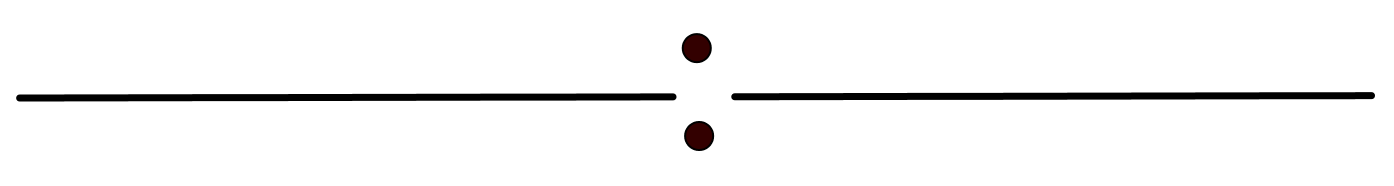
\includegraphics[width=0.4\textwidth]{doublepoint.png} 
	\end{figure}
Then this is not separated as limits, if they exist, must be unique.
	\begin{figure}[H]
	   \centering
	   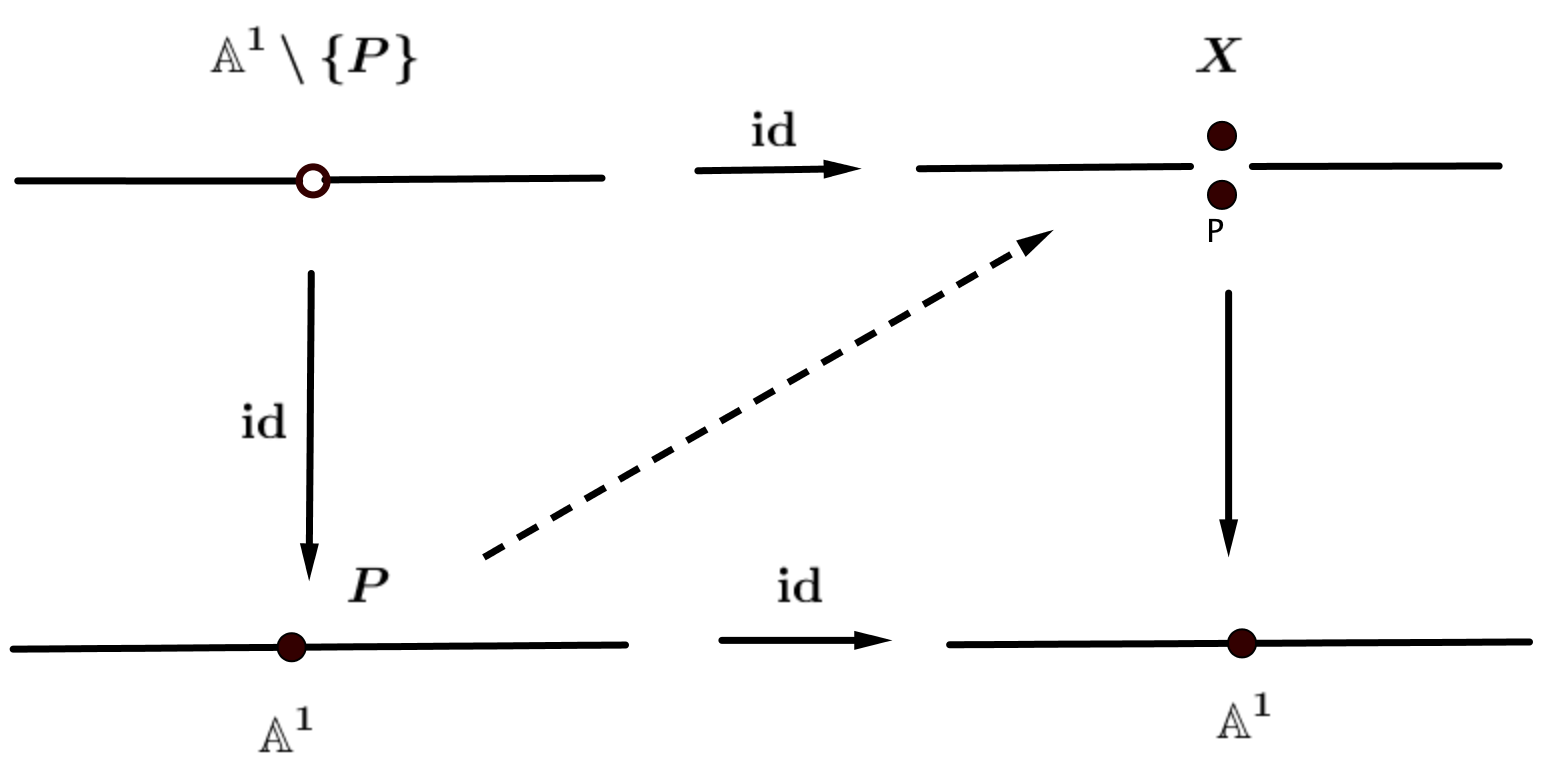
\includegraphics[width=0.5\textwidth]{doublepoint2.png} 
	\end{figure}
\end{ex}


\begin{dfn}[Stable Under Base Extension]
Let $f: X \to Y$ and $g: Y \to Y'$ be morphisms. Standard properties of the fiber product give a morphism $p_2: X \times_Y \to Y'$. Often, one denotes $p_2$ by $f'$ and $X \times_Y Y'$ by $X'$ and say $f': X' \to Y'$ is obtained from $f: X \to Y$ by base extension (change). Let $S$ be any property of a morphism. We say that $S$ is stable under base extension if and only if $f$ has $S$, then $f'$ has $S$.
\end{dfn}


\begin{prop}
Assume that the underlying schemes are noetherian:
\begin{enumerate}[(a)]
\item Open and closed immersions are separated.
\item A composition of two separated morphisms is separated.
\item Separated morphisms are stable under base extension.
\item If $f: X \to Y$ and $f': X' \to Y'$ are separated morphisms over a vase scheme $S$, then the product morphism $f \times f': X \times_S X' \to Y \times_S Y'$ is also separated.
\item If $f: X \to Y$ and $g: Y \to Z$ are two morphisms and $g \circ f$ is separated then $f$ is separated.
\item A morphism $f: X \to Y$ is separated if and only if $Y$ can be covered by open subsets $V_i$ such that $f^{-1}(V_i) \to V_i$ is separated for each $i$. 
\end{enumerate}
\end{prop}


\begin{dfn}[Proper Morphism]
A morphism $f: X \to Y$ is proper if it is separated, has finite type, and is universally closed. Here we say a morphism is closed if the image of any closed set is closed. A morphism $f: X \to Y$ is universally closed if it is closed and for any morphism $Y' \to Y$, the corresponding morphism $f': X' \to Y'$ obtained by base extension is also closed.
\end{dfn}


\begin{thmm}
Let $f: X \to Y$ be a morphism of finite type with $X$ noetherian. Then $f$ is proper if and only if for every valuation ring $R$ and for every morphism of $U$ to $X$ and $T$ to $Y$ forming a commutative diagram (using the notation as before), there exists a unique morphism $T \to X$ making the whole diagram commute. 
	\[
	\begin{tikzcd}
	U \arrow{d}{i} \arrow{r} & X \arrow{d}{f} \\
	T \arrow[dotted]{ur} \arrow{r} & Y 
	\end{tikzcd}
	\] 
\end{thmm}


\begin{ex}
Recall the blow-up of a point in $\A^n$
	\[
	\begin{tikzcd}
	X \arrow[hook]{r} \arrow[swap]{dr}{\phi} & \A^n \times \P^{n-1} \arrow{d} \\
	& \A^n
	\end{tikzcd}
	\]
$\phi$ is proper because it is projective. We took any line $L$ through $(0,\ldots,0)$ in $\A^n$ lifted $L \setminus \{(0,\ldots,0)\}$ to $X$ then took its closure $\tilde{L} \subset X$. $\tilde{L}$ met $\phi^{-1}((0,\ldots,0))$ at a point corresponding to the ``slopes'' of $L$, $\phi(\tilde{L})=L$.
	\begin{figure}[H]
	   \centering
	   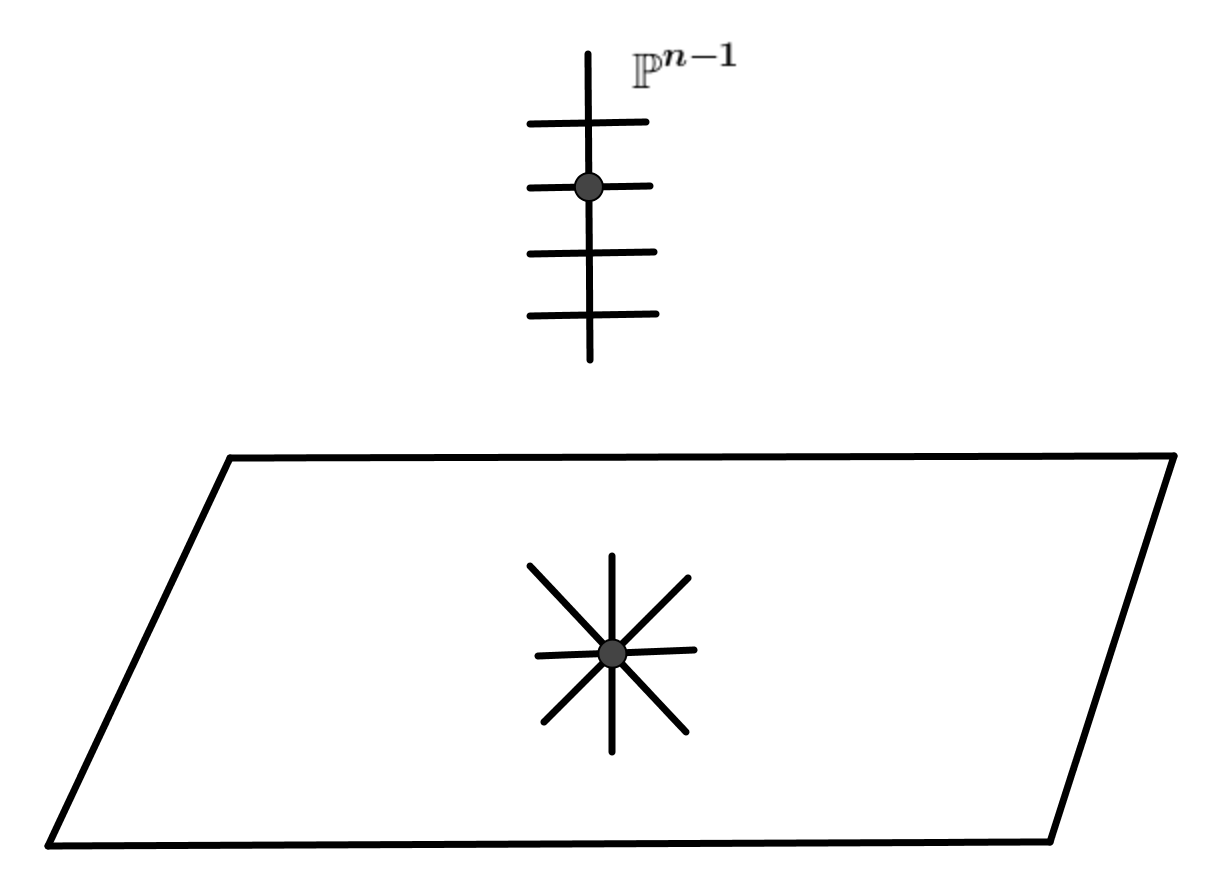
\includegraphics[width=0.5\textwidth]{projplane.png} 
	\end{figure}
If you replace $X$ by $X \setminus \{P\}$ for some $P \in \phi^{-1}((0,\ldots,0))$, it is not proper anymore. The corresponding line will not have its limit.
\end{ex}


Proper morphisms are like projective varieties. You can not get rid of something by pushing it off to $\infty$. IN $\A^2$, parallel lines do not meet because you pushed the intersection off to $\infty$. In $\P^2$, they do meet.


\begin{cor}
Assuming the underlying schemes are noetherian:
\begin{enumerate}[(a)]
\item A closed immersion is proper.
\item A composition of proper morphisms is proper.
\item Proper morphisms are stable under base extension.
\item Products of proper morphisms are proper.
\item If $f: X \to Y$ and $g: Y \to Z$ are two morphisms, $g \circ f$ is proper, and $g$ is separated then $f$ is proper.
\item Properness is local on the base.
\end{enumerate}
\end{cor}


\begin{dfn}[Projective Morphism]
If $Y$ is a scheme, we define projective $n$-space over $Y$, denoted $\P^n_Y$, to be $\P^n_\Z \times_{\spec \Z} Y$. A morphism $f: X \to Y$ of schemes is projective if it factors into a closed immersion $i: Y \hookrightarrow \P_Y^n$ for some $n$, followed by the projection $\P_Y^n \to Y$. A morphism is quasi-projective if it factors into an open immersion $j: X \to X'$ followed by a projective morphism $g: X' \to Y$. 
\end{dfn}


\begin{thmm}
A projective morphism of a noetherian scheme is proper. A quasi-projective morphism of noetherian schemes is of finite type and separated. 
\end{thmm}


Given any quasi-projective variety, you can construct the associated scheme:


\begin{prop}
Let $k$ be an algebraically closed field. The image of the functor $F: \text{Var}(k) \to \text{Sch}(k)$ (varieties over $k$ to schemes over $k$) is exactly the set of quasi-projective integral schemes of $k$. The image of the set of projective varieties is the set of projective integral schemes over $k$. In particular, for any variety $V$, $F(V)$ is an integral separated scheme of finite type over $k$. 
\end{prop}


\begin{dfn}
An abstract variety is an integral, separated scheme of finite type over an algebraically closed field $k$. If it is proper over $k$, we will also say it is complete. 
\end{dfn}


Note that complete curve is projective and every nonsingular complete surface is projective (Zariski). Finally, there exists a nonsingular complete nonprojective three-folds (Nagata, Hironata, Appendix B). But every variety can be embedded as an open dense subset of a complete variety (Nagata). So completeness is like algebra-geometric version of the analysis' compactness. 


%Pushforward of Cycles
\subsection{Push-forward of Cycles}

Let $f: X \to Y$ be a proper morphism. We want to first define $f_*: Z_k X \to Z_k Y$ and then show that $f_*(\Rat_k X) \subset \Rat_k Y$. This will give a map $f_*: A_k X \to A_k Y$ since $Z_kX$ is a free abelian group you only need to define $f_*$ on the generators. The generators are the $k$-dimensional subvarieties of $X$. Let $V$ be a $k$-dimensional subvariety of $X$. Since $f$ is proper, $f(V)$ is closed in $Y$. Continuous images of irreducible sets are irreducible and the morphisms here are continuous. Therefore, $f(V)$ is also irreducible. If the domain of a map is a reduced space, then the image is automatically reduced so $f(V)$ is a variety. Now $R(V)$ and $R(f(V))$ are both fields. Pullback of functions makes $R(f(V))$ a subfield of $R(V)$. Our assumptions on schemes, being finite type over a field, makes the relation between dimension and transcendence degrees of function fields remain valid. Then as $R(f(V)) \subset R(V)$, $\text{tr deg}_kR(f(V)) \leq \text{tr deg}_kR(V)$. But then $\dim f(V) \leq \dim V$. When $\dim f(V)=V$, this says that $R(f(V)) \subset R(V)$ is an algebraic extension of finite type over a field says that they both must be finitely generated over $k$ as finitely generated and algebraic implies finite. Then $R(f(V)) \subset R(V)$ is a finite extension and denote the degree of the extension by $[R(V):R(f(V))]$. Define
	\[
	\deg(V/f(V))=
	\begin{cases}
	[R(V):R(f(V))], & \text{if } \dim V=\dim f(V) \\
	0, \text{otherwise}
	\end{cases}
	\]
Note we cannot have $\dim f(V) > \dim V$. Let $W=f(V)$. Then we can define $f_*[V]= \deg(V/W)[W]$. This gives $f_*: Z_k X \to Z_k Y$ and if $X \ma{f} Y \ma{g} Z$, $(g \circ f)_*=g_*f_*$ because degrees of field extensions are multiplicative. If $k=\C$ or if $R(W) \subset R(V)$ is a separable extension and $k$ is algebraically closed, then $f: V \to W$ is generically a $[R(V):R(W)]$ sheeted cover. When the extension is inseparable, the cases become more pathological. When $k=\C$, this agrees with the push forward of homology in topology. 


\begin{thmm}\label{thm:ratequiv}
If $f: X \to Y$ is a proper morphism and $\alpha$ is a $k$-cycle of $X$ that is rationally equivalent to zero on $Y$, there is an induced homomorphism $f_*: A_k X \to A_k Y$ such that $A_*$ is a covariant functor for proper morphisms. 
\end{thmm}


The proof uses the fact that we may assume $\alpha=[\div r]$, where $r$ is a rational function on a subvariety of $X$. We may replace $X$ by this subvariety and replace $Y$ by $f(X)$. Therefore, we may assume $Y$ is a variety and $f$ is surjective. 


If $K \subset L$ is a finite field extension. If $a \in L$, we denote the norm of $a$ in $K$ as $N(a) \in K$. Define $f: L \to L$ by $f(x)=ax$. Now $f$ is a $k$-linear transformation. Choose a $k$-basis for $L$ and make the matrix representing the map as $M$. Define also $N(a)=\det M$. If you were to choose a different basis and get a matrix representation $M'$, $M'=PMP^{-1}$ for some invertible $P$. But then $\det(M')=\det(PMP^{-1})=\det M$, independent of the choice of basis.  


\begin{prop}
Let $f: X \to Y$ be a proper surjective morphism of varieties and let $r \in R(X)^*$. Then $f_*[\div r]=0$ if $\dim Y <\dim X$ and $f_*[\div r]=[\div(N(r))]$ if $\dim Y=\dim X$.
\end{prop}


\begin{dfn}
If $X$ is a complete scheme, i.e. $X$ is proper over $S=\Spec k$, $k$ the ground field, and $\alpha=\sum_P n_P[P]$ is a zero cycle on $X$, the degree of $\alpha$, denoted $\deg \alpha$ or $\int_X \alpha$ is defined by 
	\[
	\deg \alpha = \int_X \alpha = \sum_P n_P [R(P):k] 
	\]
Equivalently, $\deg \alpha = p_X(\alpha)$, where $p$ is the structure morphism from $X$ to $S$ and $A_0(S)=\Z[S]$ is identified with $\Z$.
	\[
	p: X \ma{\text{proper}} S=\Spec k
	\]
\end{dfn}


By Theorem~\ref{thm:ratequiv}, rationally equivalent cycles have the same degree: $\deg \div r=0$. The only way to be rationally equivalent to zero on $S=\Spec k$ is to be identically zero. We can extend the degree homomorphism to all of $A_*X$
	\[
	\int_X: A_* \to \Z
	\]
by defining $\int_X \alpha=0$ if $\alpha \in A_k X$ for $k>0$. For any morphism of complete schemes $f: X \to Y$ and any $\alpha \in A_* X$, $\int_X \alpha=\int_Y f_*(\alpha)$. Sometimes, we simply write $\int$ instead of $\int_X$. Now if $f: X \to Y$ and $g: Y \to Z$ are two morphisms, if $g \circ f$ is proper and $g$ is separated, then $f$ is proper.
	\[
	\begin{tikzcd}
	X \arrow{r}{f} \arrow{dr}{h} & Y \arrow{d}{g} \\
	& \Spec k=Z
	\end{tikzcd}
	\]
Now $X,Y$ complete say that $h,g$ are proper. Now $g \circ f=h$ is proper. But $g$ is proper and hence is separated. But then $f$ is proper. Now $\int_X \alpha=h_*\alpha$ and $\int_Y f_*(\alpha)=g_*f_*(\alpha)=h_*(\alpha)$. 


\begin{ex}
Theorem~\ref{thm:ratequiv} implies B\'ezout's Theorem for plane curves over an algebraically closed field: if $F$ and $G$ are curves of degree $m,n$ with no common components, then
	\[
	\sum_{P \in \P^2} i(P,F \cdot G) = mn
	\]
One may assume $F$ is irreducible:
	\[
	i(P,\underbrace{F_1F_2}_{F_1+F_2} \cdot G)=i(P,F_1 \cdot G)+i(P, F_2 \cdot G)
	\]
If $G$ and $G'$ have degree $n$, then $G/G'$ defines a rational function $r$ on the curve $F$ and 
	\[
	\sum i(P,F \cdot G) - \sum i(P,F \cdot G') = \sum \ord_P(r) = 0 
	\]
Assume $G$ is a product of lines. Use irreducibility to assume $G$ is a line. Then reverse the roles of $F,G$ and assume $F$ is a line. Then merely check two lines intersect at one point. 
\end{ex}


%Cycles of Subschemes
\subsection{Cycles of Subschemes}

Let $X$ be any scheme and Let $X_1,\ldots,X_t$ be the irreducible components of $X$. The local rings $\co_{X_i,X}$ are all zero-dimensional (Artinian). [The irreducible components correspond to maximal irreducible closed subsets which correspond to minimal prime ideals and when you localize you get a zero dimensional ring.] The geometric multiplicity of $X_i$ in $X$, $m_i$, are
	\[
	m_i= l_{\co_{X_i,X}} \co_{X_i,X}
	\]
The fundamental cycle $[X]$ of $X$ is the cycle $[X]=\sum_{i=1}^t m_i [X_i]$.

\begin{dfn}
If $f: X \to Y$ is a morphism and $Z$ is a subscheme of $Y$, the inverse image scheme, denoted $f^{-1}(Z)$, may be identified with the fiber product $X \times_Y Z$. 
	\[
	\begin{tikzcd}
	X \arrow[swap]{d}{f} & X \times_Y Z \arrow{l}{p_2} \arrow{d}{p_1} \\
	Y & Z \arrow[hook]{l}{i}
	\end{tikzcd}
	\]
Since $i$ is a closed embedding, $p_2$ is a closed embedding. If $I$ is the ideal sheaf of $Z$ in $Y$, then $f^{-1}(Z)$ is defined by the ideal $f^{-1}(I) \co_X$. [Note: if $U \subset Y$, then $I_Y(U) \subset \co_Y(U)$ is everything vanishing on $Y$.]
\end{dfn}

\begin{ex}
As a trivial example 
	\[
	\begin{tikzcd}
	\A^1 \arrow{r} \arrow[dash]{d} & \A^1 \arrow[dash]{d} \\
	k[x] & k[t] \arrow{l}{\phi}
	\end{tikzcd}
	\]
where $\phi(t)=x^2$.

	\begin{figure}[H]
	   \centering
	   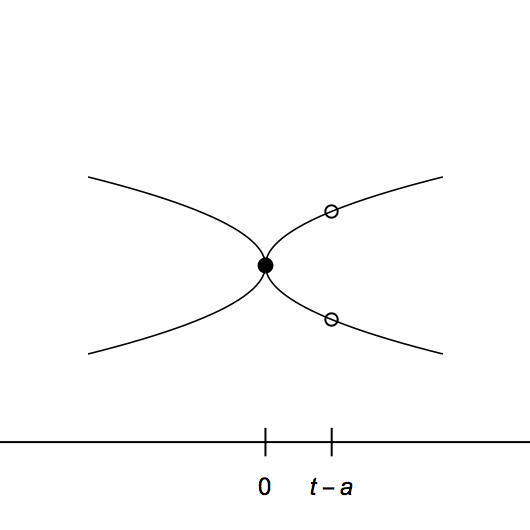
\includegraphics[width=0.5\textwidth]{parab.png} 
	\end{figure}
$x^2-a=(x-a)(x+a)$. $k[x]/(x^2)$. 	
\end{ex}

\begin{ex}
Let $V$ be a variety of dimension $k+1$ and $f: V \to \P^1$ a dominant morphism. Let $0=(1,0)$ and $\infty=(0,1)$ be the zero and infinite points of $\P^1$. The inverse image schemes $f^{-1}(0)$ and $f^{-1}(\infty)$ are purely $k$-dimensional subschemes of $V$ and the cycle $[f^{-1}(0)] - [f^{-1}(\infty)]$ correspond to the cycle $[\div f]$, where $f$ also denotes the rational function in $R(V)$ determined by the morphism $f$. $[f^{-1}(0)]$ is rationally equivalent to $[f^{-1}(\infty)]$. This is sort of like homotopy in topology where we are deforming the fiber $f^{-1}(0)$ into the fiber $f^{-1}(\infty)$. The big difference is the only 1-dimensional real manifold without boundary is $S^1$. In Algebraic Geometry, there are many 1-dimensional nonsingular projective curves. 
\end{ex}

\begin{dfn}
Two $k$-cycles $\alpha,\beta$ on $V$, a $(k+1)$-dimensional variety, are algebraically equivalent if and only if there is a dominant morphism $f: V \to Y$ where $Y$ is a nonsingular curve and two points $P,Q \in Y$ with $\alpha=[f^{-1}(P)]$, $\beta=[f^{-1}(Q)]$ rationally equivalent (hence algebraically equivalent). The converse is not true. 
\end{dfn}


%Flat Pull-back of Cycles
\subsection{Flat Pull-back of Cycles}

\begin{dfn}[Flat]
Let $f: X \to Y$ be a morphism of schemes. Let $P \in X$ be a point (closed or not) and let $Q=f(P)$. We get an induced homomorphism $f^*: \co_{Q,Y} \to \co_{P,X}$. We say that $f$ is flat at $P$ if and only if $\co_{P,X}$ is a flat $\co_{Q,Y}$ module. We say $f$ is flat if and only if it is flat at every point $P \in X$. 
\end{dfn}

Fulton gives the following (equivalent) definition:

\begin{dfn}
A morphism $f: X \to Y$ is flat if and only if for (any) $U \subset Y$, $U' \subset X$ affine open sets with $f(U') \subset U$ the induced map $f^*: A(U) \to A(U')$ makes $A(U')$ a flat $A(U)$ module. 
\end{dfn}


Recall by Algebra nonsense if $M$ is an $A$-module, then $M$ is a flat $A$-module if and only if $M_p$ is a flat $A_p$-module for all $p \in \spec A$. A morphism $f: X \to Y$ has relative dimension $n$ if and only if for all subvarieties $V$ of $Y$ and all irreducible components $V'$ of $f^{-1}(V)$, $\dim V'=\dim V+n$. If $f$ is flat, $Y$ is irreducible and $X$ has pure dimension equal to $\dim Y+n$, then $f$ has relative dimension $n$ and all base extensions $X \times_Y Y' \to Y$ have relative dimension $n$. A flat morphism is assumed to have a relative dimension. Now open immersions are flat and flatness is stable under base extensions. Compositions of flat maps are flat. 


\begin{thmm}
Let $T$ be an integral noetherian scheme. Let $X \subseteq \P^n_T$ be a closed subscheme. For each point $t \in T$, we consider the Hilbert polynomial $P_t \in \Q[z]$ of the fiber $X_t$ considered as a closed subscheme of $\P^n_{k(t)}$. Then $X$ is flat over $T$ if and only if the Hilbert polynomial is independent of $t$. 
\end{thmm}
	\[
	\begin{tikzcd}
	X \arrow[swap]{dr}{\pi} \arrow[hook]{r} & \P^n \times T \arrow{d}{p_2} \\
	& T 
	\end{tikzcd}
	\]
For $t \in T$, $p_2^{-1}(t)=\P^n$, $\pi^{-1}(t)= \P^n \cap X$ which is some closed subscheme of $\P^n$. This is a varying family of closed subschemes of $\P^n$. We know that a closed subscheme of $\P^n$ has a Hilbert polynomial. Then a map is flat if and only if the Hilbert polynomial is constant from fiber to fiber. The fibers do not vary too much  so flatness is an analog of continuously varying family. Now more examples of flat morphisms

\begin{ex}
\begin{enumerate}[(i)]
\item Open imbeddings.
\item the projection of a vector bundle or $\A^n$-bundle or projective bundle to its base.
\item the projection from a cartesian product $X=Y \times Z$ onto the first factor where $Z$ is purely $n$-dimensional scheme.
\item any dominant morphism from an $(n+1)$-dimensional variety to a nonsingular curve.
\end{enumerate}
\end{ex}

Let $f: X \to Y$ be a flat morphism of relative dimension $n$. For any subvariety $V$ of $Y$, define $f^*[V]= [f^{-1}(V)]$. This gives $f^*: Z_kY \to Z_{k+n} X$. 

\begin{lem}
If $f: X \to Y$ is flat, then for any subscheme $Z$ of $Y$
	\[
	f^*[Z] = [f^{-1}(Z)]
	\]
\end{lem}


\begin{thmm}
Let $f: X \to Y$ be flat morphism of relative dimension $n$ and $\alpha$ a $k$-cycle of $Y$ which is not rationally equivalent to 0. Then $f^* \alpha$ is rationally equivalent to zero in $Z_{k+n}X$. There are therefore induced homomorphisms, the flat pull-backs, $f^*: A_k Y \to A_{k+n}X$, so that $A_*$ becomes a contravariant functor for flat morphisms. 
\end{thmm}

Suppose $f: X \to Y$ is both proper and flat of relative dimension $n>0$. For $\alpha \in A_kY$, what is $f_*f^*\alpha$? Let $V$ be a $k$-dimensional subvariety of $Y$. Then $f^{-1}(V)$ has dimension $k+n$. East set theory says $f(f^{-1}(V))=V$. In proper push forwards, what was $f_*[W]$ when $\dim W >\dim f(W)$ -- 0! Then $f_*f^*\alpha =0$. What about $n=0$? 

\begin{dfn}]Finite Morphism]
A morphism $f: X \to Y$ is a finite morphism if there exists a covering of $Y$ by affine subsets $V_i = \spec B_i$ such that for each $i$, $f^{-1}(V)$ is affine, equal to $\spec A_i$, where $A_i$ is a $B_i$-algebra which is a finitely generated $B_i$-module.
\end{dfn}

This is true for every open affine in $Y$. We say that $f$ is quasi-finite if and only if for every point $P \in Y$, $f^{-1}(P)$ is finite. It is true that every finite morphism is quasi-finite. However, the converse is not true. Furthermore, it is the case that every finite morphism is proper. 

\begin{ex}
Let $f: X' \to X$ be a finite and flat morphism. Each point of $X$ having a neighborhood $U$ such that the coordinate ring of $f^{-1}(U)$ is a finitely generated module over the coordinate ring of $U$. One says that $f$ has degree $d$ if the rank of this module is $d$, for all such $U$. Then for all subvarieties $U$ of $X$, $f_*f^*[V]=d[V]$ in $Z_*(X)$. The composite
	\[
	A_*X \ma{f^*} A_*X' \ma{f_*} A_*X
	\]
is multiplication by $d$. 
\end{ex}





%An Exact Sequence
\subsection{An Exact Sequence}

\begin{prop}
Let $Y$ be a closed subscheme of a scheme $X$ and let $U= X \setminus Y$, $i: Y \to X$, $j: U \to X$ the inclusions. The sequence
	\[
	A_kY \ma{i_*} A_kX \ma{j^*} A_k U \ma{} 0
	\]
is exact for all $k$. 
\end{prop}

\pf We show
	\[
	Z_k Y \ma{} Z_k X \ma{} Z_k U \ma{} 0
	\]
is exact. We show that $Z_k X$ surjects onto $Z_kU$. If $Y$ is a closed subvariety of $Y$, then $\overline{V}$, its closure in $X$, is a subvariety of $X$ with $j^*[\overline{V}]=[V]$. For any closed subvariety $V$ of $X$, $V \cap U$ is either empty (if $V \subset Y$) or a subvariety of $U$. This shows $Z_kY$ surjects onto the kernel. What more do you need to show to get the $A_k$'s? 
	\[
	\begin{tikzcd}
	Z_k X \arrow[two heads]{r} \arrow{d} & Z_k U \arrow{d} \\
	A_k X \arrow[two heads]{r} & A_k U
	\end{tikzcd}
	\]
This certainly implies that we need to check that $A_kY$ still surjects onto the kernel. Let $\alpha \in A_k X$. Assume $f^*\alpha \sim 0$ in $A_kU$. Then $f^*\alpha= \sum [\div r_i]$ and the $r_i$ are rational functions on $k+1$ dimensional subvarieties $V_i$ of $U$. Then $R(V_i)=R(\overline{V}_i)$, where $\overline{V}_i$ is the closure of $V_i$ in $X$. What does $\div(r_i)$ look like on $\overline{V}_i$? Say in $V$ $\div(r_i)= \sum n_j [W_j]$. In $\overline{V}$, $\div(r_i)=\sum n_j [\overline{W}_j] + \sum m_s [W_s]$, $W_s \subset Y$. Now $\alpha$ is the first sums plus perhaps some things from $Y$. So up to changing things in $Y$, $\alpha$ is $\sum n_j [\overline{W}_j]$. Then modifying $\alpha$, we can see that $\alpha \sim 0$. 





%Affine Bundles
\subsection{Affine Bundles}

\begin{dfn}
Let $Y$ be a scheme and let $p: X \to Y$ be a morphism. We say $p: X \to Y$ is an affine bundle over $Y$ under the following conditions: 
	\begin{enumerate}[(i)]
	\item there is an open cover $\{U_\alpha\}$ of $Y$ such that $p^{-1}(U_\alpha) \cong U_\alpha \times \A^n$
	\item $p$ restricted to $p^{-1}(U_\alpha)$ is the projection onto the first factor. 
	\end{enumerate}
\end{dfn}

Note that in this case, $p$ will be flat of relative dimension $n$.

\begin{prop}
Let $p: E \to X$ be an affine bundle of rank $n$. Then the flat pull-back
	\[
	p^*: A_k X \to A_{k+n} E
	\]
is surjective for all $k$.
\end{prop}

\pf Let $U$ be an open set of $X$ for which $p^{-1}(U) \cong U \times \A^n$. Let $Y= X \setminus U$. We have the following commutative diagram:
	\[
	\begin{tikzcd}
	A_k(Y) \arrow{d} \arrow{r} & A_k(X) \arrow{r} \arrow{d} & A_k(U) \arrow{d} \arrow{r} & 0 \\
	A_kp^{-1}(Y) \arrow{r} & A_kp^{-1}(X)=E \arrow{r} & A_kp^{-1}(U)=U \times \A^n \arrow{r} & 0 
	\end{tikzcd}
	\]
Now $p(Y) \to Y$ is an affine bundle with base of lower dimension. Therefore, if we can show this for $p: U \times \A^n \to U$, the proof will be complete. But this will be true if one can show it for $p: U \times \A^1 \to U$. This is left to the reader. \qed \\
	

\begin{cor}
	\[
	A_k(\A^n)=
	\begin{cases}
	\Z, & k=n \\
	0, & \text{otherwise}
	\end{cases}
	\]
\end{cor}

\pf We already know $A_n(\A^n)=\Z$. Now $p: \A^n \to \spec k$ is an affine bundle of rank $n$.
	\[
	A_k \spec k =
	\begin{cases}
	\Z, & k=0 \\
	0, & \text{otherwise}
	\end{cases}
	\]
By surjectivity we get $A_k\A^n=0$ for $k<n$. If $k=n$, we obtain a quotient of $\Z$. \qed \\





%Exterior Products
\subsection{Exterior Products}


Recall our schemes are always schemes over a field. When we write $X \times Y$, we will mean $X \times_{\spec k} Y$. We have a map $Z_k X \otimes Z_l Y \to Z_{k+l}(X \times Y)$ given by $[V] \otimes [W] \to [V \times W]$. If $k$ is not algebraically closed, $V \times W$ need not be irreducible even if $V$ and $W$ are. We had defined the cycle associated to a subscheme. You may need to use this for $[V \times W]$. 


\begin{prop} \hfill
\begin{enumerate}[(a)]
\item If $\alpha \sim 0$ or $\beta \sim 0$ then $\alpha \times \beta \sim 0$ (change $Z$ to $A$)
\item Let $f: X' \to X$ and $g: Y' \to Y$ be morphisms, $f \times g$ the induced morphism from $X' \times Y' \to X \times Y$. If $f$ and $g$ are proper morphisms, so is $f \times g$ and $(f \times g)_*(\alpha \times \beta)= f_*\alpha \times g_*\beta$. 
\item If $f$ and $g$ are flat of relative dimensions $m$ and $n$, then $f \times g$ is flat of relative dimension $m+n$ and $(f\times g)^*(\alpha \times \beta)=f^*\alpha \times g^*\beta$ for all cycles $\alpha$ on $X$ and $\beta$ on $Y$. 
\end{enumerate}
\end{prop}
% !TEX root = ../../intersection_theory.tex

\newpage
%Divisors 
\section{Divisors}


First, a bit of background. 

\begin{dfn}[Sheaf Modules]
Let $(X,\co_X)$ be a ringed space. A sheaf of $\co_X$-modules (or simply an $\co_X$-module) is a sheaf $\cf$ on $X$ such that for each open set $U \subseteq X$, the group $\cf(U)$ is an $\co_X(U)$-module and for each inclusion of open sets $V \subseteq U$, the restriction homomorphism $\cf(U) \to \cf(V)$ is compatible with the module structure via the ring homomorphism $\co_X(U) \ma{\rho_{U,V}} \co_X(V)$: $a \in \cf(U)$, $r \in \co_X(U)$, then $\rho_{U,V}(ra)=\rho_{U,V}(r) \rho_{U,V}(a)$. 
	\[
	\begin{tikzcd}
	\co_X(V) \times \cf(V) \arrow{d}{\rho_{V,U} \times \rho_{V,U}} \arrow{r} & \cf(V) \arrow{d} \\
	\co_X(U) \times \cf(U) \arrow{r} & \cf(U)
	\end{tikzcd}
	\] 
\end{dfn}


\begin{dfn}[Morphism]
A morphism $\cf \to \cg$ of sheaves of $\co_X$-modules is a morphism of sheaves such that for each open set $U \subseteq X$, the map $\cf(U) \to \cg(U)$ is a homomorphism of $\co_X(U)$-modules. 
\end{dfn}


Note that the kernel, cokernel, and image of a morphism of $\co_X$-modules is again an $\co_X$-module is again an $\co_X$-module. If $\cf'$ is a subsheaf of $\co_X$-modules fo an $\co_X$-module $\cf$, then the quotient sheaf $\cf/\cf'$ is an $\co_X$-module. Any direct sum, product, limit, or inverse limit of $\co_X$-modules is an $\co_X$-module. If $\cf$ and $\cf$ are two $\co_X$-modules, we denote the group of morphisms from $\cf$ to $\cg$ by $\Hom_{\co_X}(\cf,\cg)$ or sometimes $\Hom_X(\cf,\cg)$. A sequence of $\co_X$-modules and morphisms is exact if and only if it is exact as a sequence of sheaves of abelian groups. 

If $U$ is an open subset of $X$ and if $\cf$ is an $\co_X$-module, then $\cf|_U$ is an $\co_X$-module. If $\cf$ and $\cg$ are two $\co_X$-modules, the presheaf $U \mapsto \Hom_{\co_X|U}(\cf|_U,\cg|_U)$ is a sheaf, which we call the sheaf Hom and denote by $\Hom_{\co_X},(\cf,\cg)$. It is also an $\co_X$-module. We define the tensor product of two $\co_X$-modules as the sheaf associated to the presheaf $U \mapsto \cf(U) \otimes_{\co(X)} \cg(U)$. Sometimes, we write $\cf \otimes \cg$. An $\co_X$-module $\cf$ is free if and only if it is isomorphic to a direct sum of copies of $\co_X$. It is locally free if $X$ can be covered by open sets $U$ for which it is a free $\co_X|_U$ module. It is important to know that locally free does not imply free. In that case the rank of $\cf$ on such an open set is the number of copies of the structure sheaf needed (finite or infinite). If $X$ is connected, the rank of a locally free sheaf is the same everywhere. We call this the rank of the sheaf. A locally free sheaf of rank 1 is called an invertible sheaf. A sheaf of ideals on $X$ is a sheaf of modules $\ci$ which is a subsheaf of $\co_X$. In other words for every open set $U$, $\ci(U)$ is an ideal in $\co_X(U$). Let $f: (X,\co_X) \to (Y,\co_Y)$ be a morphism of ringed spaces. If $\cf$ is an $\co_X$-module, then $f_*\cf$ is an $f_*\co_X$-module. Since we have the morphism $f^\#: \co_Y \to f_*\co_X$ of sheaves of rings on $Y$, this gives $f_*\cf$ a natural structure of $\co_Y$-module. We call it the direct image of $\cf$ by the morphism $f$. Now let $\cg$ be a sheaf of $\co_X$-modules. Then $f^{-1}\cg$ is an $f^{-1} \co_Y$-module. Because of the adjoint property of $f^{-1}$, we have a morphism $f^{-1} \co_Y \to \co_X$ of sheaves of rings on $X$. We define $f^*\cg$ to be the tensor product $f^{-1}\cg \otimes_{f^{-1}\co_Y} \co_X$. Note that if we have a map $f: A \to B$ and $N$ and $M$ are $A,B$-modules, respectively. A module over $B$ is automatically a module over $A$. Is there a way to make a module over $A$ into a module over $B$? If $N$ and $B$ are both $A$-modules, then $N \otimes_A B$ is a $B$-module. Thus, $f^*\cg$ is an $\co_X$-module. We call it the inverse image of $\cg$ by the morphism $f$. 


Now onto schemes. 


\begin{dfn}
Let $A$ be a ring and $M$ an $A$-module. We define the sheaf associated to $M$ on $\spec A$, denoted by $\tilde{M}$, as follows: for each prime ideal $p \subseteq A$, define $M_p$ to be the localization of $M$ at $p$. For any open set $U \subseteq \spec A$. We define the group $\tilde{M}(U)$ to be the set of functions $s: U \to \sqcup_{p \in U} M_p$ such that for each $p \in U$, $s(p) \in M_p$ and such that $s$ is locally a fraction $m/f$ with $m \in M$ and $f \in A$. To be precise, we require that for each $p \in U$, there is a neighborhood $V$ of $p$ in $U$ and there are elements $m \in M$ and $f \in A$ such that for each $q \in V$, $f \notin q$, and $s(q)=m/f$ in $M_q$. We make $\tilde{M}$ into a sheaf using the obvious restriction maps. 
\end{dfn}


Note that when $M=A$, you get $\co_X$. 

\begin{prop}
Let $A$ be a ring, $M$ an $A$-module, and $\tilde{M}$ be the sheaf on $X=\spec A$ associated to $M$, then:
	\begin{enumerate}[(a)]
	\item $\tilde{M}$ is an $\co_X$-module
	\item for each $p \in X$, the stalk $(\tilde{M})_p$ of the sheaf $\tilde{M}$ at $p$ is isomorphic to the localization module $M_p$. 
	\item for any $f \in A$, the $A_f$-module $\tilde{M}(D(f))$ is isomorphic to the localization module $M_f$
	\item in particular, $\Gamma(X,\tilde{M}) \cong M$.
	\end{enumerate}
\end{prop}


\begin{dfn}[Coherent]
Let $(X,\co_X)$ be a scheme. A sheaf of $\co_X$-modules $\cf$ is quasi-coherent if $X$ can be covered by open affine subschemes $U_i=\spec A_i$ such that for each $i$ there is an $A_i$-module $M_i$ with $\cf\big|_{U_i} \cong \tilde{M}_i$. We say that $\cf$ is coherent if furthermore each $M_i$ can be taken to be a finitely generated $A_i$-module. 
\end{dfn}


\begin{ex}
On any scheme $X$, the structure each $\co_X$ is quasi-coherent and in fact coherent. Take $A_i=M_i$.
\end{ex}


\begin{exc}
Show that a sheaf of $\co_X$-modules $\cf$ on a scheme $X$ is quasi-coherent if and only if every point of $X$ has a neighborhood $U$ such that $\cf\big|_U$ is isomorphic to a cokernel of a morphism of free sheaves on $U$. If $X$ is noetherian, then $\cf$ is coherent if and only if it is locally a cokernel of a morphism of free sheaves of finite rank. [These properties were originally the definition of quasi-coherent and coherent sheaves.] 
	\[
	\co_X\big|_{U}^{m_i} \ma{} \co_X\big|_{U}^{n_i} \ma{} \cf\big|_U \ma{} 0
	\]
$m_i,n_i$ perhaps $\infty$ for quasi-coherent. Now if $m_i,n_i<\infty$, then it is coherent. You must assume noetherian usually for coherent to be much better than quasi-coherent.
\end{exc}


\begin{prop}
Let $X$ be a scheme. Then a $\co_X$-module $\cf$ is quasi-coherent if and only if for every open affine subset $U=\spec A$ of $X$, there is an $A$-module $M$ such that $\cf\big|_U \cong \tilde{M}$. If $X$ is noetherian, then $\cf$ is coherent if and only if the same is true with the extra condition that $M$ be a finitely generated $A$-module. 
\end{prop}


\begin{prop}
Let $X$ be a scheme. The kernel, cokernel, and image of any morphism of quasi-coherent sheaves are quasi-coherent. Any extension of quasi-coherent sheaves is quasi-coherent. If $X$ is noetherian, the same is true for coherent sheaves. 
\end{prop}


\begin{prop}
Let $f: X \to Y$ be a morphism of schemes. 
	\begin{enumerate}[(a)]
	\item if $\cg$ is a quasi-coherent sheaf of $\co_Y$-modules, then $f^*\cg$ is a quasi-coherent sheaf of $\co_X$-modules.
	\item if $X$ and $Y$ are noetherian and $\cg$ is cohere, then $f^*\cg$ is coherent.
	\item Assume that either $X$ is noetherian or $f$ is quasi-compact and separated, then $\cf$ is a quasi-coherent sheaf of $\co_X$-modules, $f_*\cf$ is a quasi-coherent sheaf of $\co_Y$-modules.
	\end{enumerate}
\end{prop}


\begin{rem}
If $X$ and $Y$ are noetherian, it is not true in general that $f_*$ of a coherent sheaf is coherent. However, it is true that if $f$ is a finite morphism or a projective morphism or more generally a proper morphism. 
\end{rem}


\begin{dfn}
Let $Y$ be a closed subscheme of a scheme $X$ and $i: Y \to X$ be the inclusion morphism. We define the ideal sheaf of $Y$, denoted $\ci_Y$, to be the kernel of the morphism $i^\#: \co_X \to i_* \co_Y$. 
\end{dfn}


\begin{prop}
Let $X$ be a scheme. For a closed subscheme $Y$ of $X$, the corresponding ideal sheaf $\ci_Y$ is a quasi-coherent sheaf of ideals of $X$. If $X$ is noetherian, it is coherent. Conversely, any quasi-coherent sheaf of ideals on $X$ is the ideal sheaf of a uniquely determined closed subscheme of $X$.
\end{prop}


\begin{exc}
Let $X$ be a noetherian scheme and let $\cf$ be a coherent sheaf (on $X$).
	\begin{enumerate}[(a)]
	\item if the stalk $\cf_X$ is a free $\co_X$-module for some point $x \in X$, then there is a neighborhood $U$ of $x$ such that $\cf\big|_U$ is free.
	\item $\cf$ is locally free if and only if the stalks $\cf_X$ are free $\co_X$-modules for all $x \in X$.
	\item $\cf$ is invertible, i.e. locally free of rank 1, if and only if there is a coherent sheaf $\cg$ such that $\cf \otimes \cg \cong \co_X$. [This justifies the terminology invertible: it means that $\cf$ is an invertible element of the monoid of coherent sheaves under the operation $\otimes$.]
	\end{enumerate}
[Hint: $\cg$ is the dual of $\cf$. $\tilde{\cf} = \Hom_{\co_X}(\cf,\co_X)$.]
\end{exc}


Isomorphism classes of locally free rank one sheaves form a group under $\otimes$. The identity is $\co_X$ and $M \otimes_A A \cong M$. Sometimes, this is denoted $\Pic X$, the Picard group of $X$. The line bundles, up to isomorphism, are equivalent to locally free sheaves of rank 1, up to isomorphism. These are both equivalent to Cartier divisors module rational equivalences. 


\begin{exc}
Let $Y$ be a scheme and let $\mathcal{S}$ be a quasi-coherent sheaf of $\co_Y$-algebras, i.e. a sheaf of rings which is at the same time a quasi-coherent sheaf of $\co_Y$-modules. Show that there is a unique scheme $X$ and a morphism $f: X \to Y$ such that for every affine open $V \subseteq Y$, $f^{-1}(V) \cong \spec \mathcal{S}(V)$ and for every inclusion $U \to V$ of open affines of $Y$, the morphism $f^{-1}(U) \to f^{-1}(V)$ corresponds to the restriction homomorphism $\mathcal{S}(V) \to \mathcal{S}(U)$. The scheme is called $\spec A$. [Hint: Construct $X$ by gluing together schemes $\spec \mathcal{S}(V)$ for $V$ open affine in $Y$.] $V=\spec A$ and $\mathcal{S}(V)$ must be an $A$-algebra. Now $\mathcal{S}(V)$ is a ring and $A \to \mathcal{S}(V)$ so there is a map $\spec \mathcal{S}(V) \to \spec A=V$.
\end{exc}


For modules $M$ and $A$, recall the tensor algebra of $M$, $\oplus_{i=0}^\infty M^{\otimes i}$ and the symmetric algebra $\oplus_{i=0}^\infty \text{Sym}^i(M)$. If $M$ is free of rank $n$, $\text{Sym}(M)=A[x_1,\ldots,x_n]$. You can do this all for sheaves of $\co_X$-modules. 


\begin{exc}
Let $Y$ be a scheme. A (geometric) vector bundle of rank $n$ over $Y$ is a scheme $X$ and a morphism $f: X \to Y$, together with additional data consisting of an open covering $\{U_i\}$ of $Y$ and isomorphisms $\psi_i: f^{-1}(U_i) \to \A^n_{U_i}= \A^n \times U_i$, such that for any $i,j$ and any open affine subset $V=\spec A \subseteq U_i \cap U_j$ (remembering the affine opens are a base for the topology) the automorphism $\psi=\psi_j \circ \psi_i^{-1}$ of $\A^n_V=\spec A[x_1,\ldots,x_n]$ is given by a linear automorphism $\theta$ of $A[x_1,\ldots,x_n]$, i.e. $\theta(a)=a$ for any $a \in A$ and $\theta(x_i)=\sum a_{ij} x_j$ for suitable $a_{ij} \in A$. 
	\begin{enumerate}[(a)]
	\item Let $\mathcal{E}$ be a locally free sheaf of rank $n$ on a scheme $Y$. Let $S(\mathcal{E})$ be the symmetric algebra on $\mathcal{E}$ and let $X=\spec S(\mathcal{E})$ with projection morphism $f: X \to Y$. For each affine open subset $U \subseteq Y$ for which $\mathcal{E}\big|_U$ is free, choose a basis of $\mathcal{E}$ and let $\psi: f^{-1}(U) \to \A^n_U$ be the isomorphism resulting from the identification of $S(\mathcal{E}(U))$ with $\co(U)[x_1,\ldots,x_n]$. Then $(X,f,\{U_i\},\{\psi_i\})$ is a vector bundle of rank $n$ over $Y$ which does not depend on the basis of $\mathcal{E}(U)$ chosen. We call it the geometric vector bundle associated to $\mathcal{E}$ and denote it by $V(\mathcal{E})$.
	\item For any morphism $f: X \to Y$ a section of $f$ over an open set $U\subseteq Y$ is a morphism $s: U \to X$ such that $f \circ s=1_U$. It is clear how to restrict sections to smaller open sets or how to glue them together so to see that the presheaf $U \mapsto$ the set of sections over $U$ is a sheaf of sets on $Y$ which we denote by $\mathcal{I}(X\setminus Y)$. Show that if $f: X \to Y$ is a vector bundle of rank $n$ then the sheaf of sections $\mathcal{I}(X \setminus Y)$ has a natural structure of $\co_Y$-modules which makes it a locally free $\co_Y$-module of rank $n$.
	\item Show that these are the `reverse' to each other. 
	\end{enumerate}
\end{exc}


\begin{dfn}
A vector bundle $E$ of rank $r$ on a scheme $X$ is a scheme $E$ equipped with a morphism $\pi: E \to X$ satisfying the following condition: there must be an open covering $\{U_i\}$ of $X$ and isomorphisms $\phi_i$ of $\pi^{-1}(U_i)$ with $U_i \times \A^r$ over $U_i$ such that over $U_i \cap U_j$ the composites $\phi_i \circ \phi_j^{-1}$ are linear, i.e. given by a morphism $g_{ij}: U_i \cap U_J \to \text{GL}(r,k)$. These transition functions satisfy
	\[
	g_{ik}= g_{ij} g_{jk}, \quad g_{ij}^{-1}=g_{ji}, \quad g_{ii}=1
	\]
Conversely, any such transition functions determine a vector bundle. 
\end{dfn}


Now let $X$ be a $n$-dimensional variety. [Although, what will follow could be done for any algebraic scheme.] 

\begin{dfn}[Weil/Cartier Divisor]
A Weil divisor on $X$ is an element of $Z_{n-1} X$. A Cartier divisor on $X$ is defined by data $(U_\alpha,f_\alpha)$ where the $U_\alpha$ form an open (affine) covering of $X$ and the $f_\alpha$ are nonzero functions in $R(U_\alpha)=R(X)$, subject to the condition that $f_\alpha/f_\beta$ is a unit, i.e. regular, nowhere vanishing function on $U_\alpha \cap U_\beta$. The rational functions $f_\alpha$ are called local equations of $D$ (the Cartier divisors); they are well defined up to multiplication by units on $U_\alpha$. If you replace $f_\alpha$ by $g_\alpha f_\alpha$, where $g_\alpha$ is a regular nowhere vanishing function on $U_\alpha$, we call that the same divisor. 
\end{dfn}


When do $(U_\alpha,f_\alpha)$, $(U_\beta,h_\beta)$ give the same Cartier divisor? 
	\[
	\begin{split}
	(U_\alpha, f_\alpha) \ma{\simeq} (U_\alpha \cap U_\beta, f_\alpha) \\
	(U_\beta, h_\beta) \ma{\simeq} (U_\alpha \cap U_\beta, h_\alpha) 
	\end{split}
	\]
These two need to be the same by the previous criterion. Now when is a Cartier divisor a Weil divisor? If $D$ is a Cartier divisor on $X$ and $V$ is a subvariety of $X$ of codimension one, write $\ord_V D= \ord_V f(\alpha)$, where $\ord_V$ is the order function on $R(X)$, $f_\alpha$ is the local equation for $D$ on $U$, where $U_\alpha \cap V \neq \emptyset$, multiplying $f_\alpha$ by $g_\alpha$ -- a regular nowhere vanishing function on $U_\alpha$ -- does not change the order: given another $U_\beta$, $U_\beta \cap V \neq \emptyset$ and $\ord_V(f_\beta)=\ord_V(f_\alpha)$ as $f_\alpha/f_\beta$ is a unit on $U_\alpha \cap U_\beta$. Define $[D]$ the Weil divisor associated to $D$ by 
	\[
	[D]=\sum_{\substack{V \subset X \text{ codim}\\ \text{1 subvariety}}} \ord_V D[V]
	\]
The sum is finite for the same reason the divisor of a rational function is finite. 


You can make the Cartier divisors into a group, $\Div(X)$: $D$, $(U_\alpha,f_\alpha)$, $E$, $(U_\alpha,g_\alpha)$, then $D+E=(U_\alpha,f_\alpha g_\alpha)$. Since $\ord_V$ is additive, $\ord_V(f_\alpha g_\alpha)= \ord_V f_\alpha + \ord_V g_\alpha$. Therefore, there is a group homomorphism $\Div(X) \to Z_{n-1}(X)$.


Given $f \in R(X)^*$, you make a Cartier divisor $(X,f)$. These form a subgroup of $\Div(X)$. The Weil divisors associated to this are $\div(f)$. Define two Cartier divisors $D,D'$ to be linearly equivalent if and only if $D' - D=\div f$; the Picard group is defined as $\Pic(X):= \Div(X)/\text{linear equivalence}$. We get a homomorphism $\Pic(X) \top A_{n-1} X$. The homomorphism is in general neither injective nor surjective. The problem is that codimension 1 subvarieties that are locally defined by one equation. 
If $X$ is nonsingular, then all codimension subvarieties are locally defined by an equation so that it is an isomorphism. Recall that in Hartshorne, there is a theorem about intersecting a subvariety of $\P^n$ with a hypersurface in $\P^n$. One thing that made the theorem work was that a hypersurface was defined by one equation. Cartier divisors generalize this---they are locally defined by a single equation. We will see that we can intersect any cycle in $Z_*X$ with a Cartier divisor. There is not a good way to intersect with Weil divisors. 


The support of a Cartier divisor $D$, denoted $\supp(D)$ or $|D|$ is the union of all subvarieties $Z$ of $X$ such that the local equation for $D$ in the local ring $\co_{Z,X}$ is not a unit. This is a closed algebraic subset of $X$. On a general scheme $X$, an effective Cartier divisor is a subscheme which is locally defined by one equation, which is required to be a non-zerodivisor. Now a locally free sheaf of rank 1 is the same as an invertible sheaf which is the same as line bundles. The special case of locally free sheaves of rank $n$ are the same as vector bundles of rank $n$. We want to bring Cartier divisors into this. That is, we want Cartier divisors on arbitrary schemes. Let $X$ be an algebraic scheme. For each affine open set $U$ of $X$, let $K(U)$ be the total quotient ring of the coordinate ring $A(U)$, i.e. the localization of $A(U)$ at the multiplicative system of elements which are not zerodivisors. This determines a presheaf on $X$ whose associated sheaf is denoted $\K$.


Let $\K^*$ denote the multiplicative sheaf of invertible elements in $\K$ and $\co^*$ the sheaf of invertible elements in $\co=\co_X$. A Cartier divisor $D$ on $X$ is a section of the sheaf $\K^*/\co^*$, this means a global section---an element of $\K^*/\co^*(X)$. Connect this with the other definition: an affine open cover $\{U_i\}$ of $X$. If $f_i \in K(U_i)$, then $f_i/f_j$ was a unit on $U_i \cap U_j$. Do the $f_i$ fit together to give a global section of $\K$ or $\K^*$? Do they agree on overlaps? Not quite, but they do agree up to elements of $\co^*(U_i \cap U_j)$. So they do fit together to give a section over $X$ of $\K^*/\co^*$. A Cartier divisor $D$ on a scheme $X$ determines a line bundle on $X$, denoted $\co_X(D)$ or $\co(D)$. The sheaf of sections of $\co(D)$ may be defined to be the $\co_X$-subsheaf of $\K$ generated on $U_i$ by $f_i^{-1}$. [This gives a locally free sheaf of rank 1.] Equivalently, the transition functions for $\co(D)$ with respect to the covering $U_i$ are $g_{ij}= f_i/f_j$. Therefore, we have the following diagram
	\[
	\begin{tikzcd}
	\text{line bundle} \arrow{rr} \arrow[dotted,yshift=0.5ex]{dr} & & \text{locally free rank 1} \arrow{ll} \arrow[dotted,yshift=-1ex]{dl} \\
	& \text{Cartier divisor} \arrow[yshift=-1ex]{ul} \arrow[yshift=0.5ex]{ur} & 
	\end{tikzcd}
	\]
The dotted arrows do not always work but the scheme has to be rather `weird' for these not to be all solid arrows. If the locally free rank 1 sheaf is a subsheaf of $\K$, you can go backwards. The local generators can be taken as $f_i$ for your divisor. If $\cf \subset \K$, $\cf$ is free of rank 1 over $U_i$: take a basis (one element) for $\cf(U)$ over $\co(U_i)$, $f_i \in \K(U_i)$. These $f_i$ define a Cartier divisor. For most reasonable schemes, every locally free rank 1 sheaves are isomorphic to subsheaves of $\K$. On a scheme where every Cartier divisor is Weil, then line bundles are Weil there is a map from line bundles to Weil divisors by taking the divisor of a rational section. 


\begin{ex}[EGA, IV.21.6]
If $X$ is normal (respectively, locally factorial) then $\Div X \to Z_{n-1} X$ and $\Pic X \to A_{n-1} X$ are injective (respectively, isomorphisms). Recall that $X$ is normal if and only if for every affine open $\Spec A \subset X$, $A$ is integrally closed in its quotient field. Recall also that $X$ is locally factorial if and only if every point $P \in X$, the local ring $\co_{P,X}$ is a UFD. 
\end{ex}


Recall from commutative algebra that a regular local ring is a UFD and in a UFD that every height 1 prime is principal. 


\begin{ex}
Let $X$ be the projective curve over $\C$ defined by the homogeneous equation $y^2z=x^3$. Then $A_0X \cong \Z$ and the homomorphism $\Pic X \to A_0X$ is surjective with kernel the additive group of $\C$. In the case that $X$ is the curve $y^2z=x^2z+^3$, the kernel is $\C^*$.
\end{ex}


\begin{ex}
Take the curve $y^2z=x^3$ on the affine patch $z=1$. Then we have the cusp $y^2=x^3$. 
	\[
	k[x,y]/(y^2-x^3) \cong k[t^2,t^3]
	\]
The ideal $(t^2,t^3)$ is the ideal of the origin, which is not principal. If you blow up the point, you resolve the singularity: $\P^1 \to X$ surjects and $\P^1 \setminus \{\text{point}\}$ is isomorphic to $\C$. 
\end{ex}


\begin{ex}
Let $X$ be the surface in $\A^2$ defined by the equation $z^2=xy$. The line $z=x=0$ (a generator for the cone) defines a Weil divisor which is not a Cartier divisor. In this case, $\Pic X=0$ and $A,X= \Z/2\Z$. 
\end{ex}





%Line Bundles and Pseudo-Divisors
\section{Line Bundles and Pseudo-Divisors}


Cartier divisors are nice as one can always intersect with them. However, you can not always pull them back via morphism $f: X \to Y$. Say $D$ is a Cartier divisor on $Y$. If not component of $|D|$ contains any component of $f(X)$, you can define $f^*D$ as a Cartier divisor on $X$ by pulling back all the local equations. But if some component of $f(x) \subset |D|$, then some equations that define $D$ pull back to something that vanishes on a component of $X$ and you do not get a divisor. 


\begin{dfn}[Pseudo-Divisor]
A pseudo-divisor on a scheme $X$ is a triple $(L,Z,s)$, where $L$ is a line bundle on $X$, $Z$ is a closed subset of $X$, and $s$ is a nowhere vanishing section of $L$ on $X\setminus Z$ (equivalently, $s$ is a trivialization of the restriction of $L$ to $X \setminus Z$). [If you pick at random on $X, L, Z$, you probably cannot find $s$ so that $(L,Z,s)$ is a pseudo-divisor.] We call $L$ the line bundle, $Z$ the support, and $s$ the section of the pseudo-divisor. Data $(L',Z',s')$ define the same pseudo-divisor if $Z=Z'$ and there is an isomorphism $\sigma$ of $L$ with $L'$ such that the restriction of $\sigma$ to $X \setminus Z$ takes $s$ to $s'$. 
\end{dfn}


Note that a pseudo-divisor with support $X$ is simply an isomorphism class of line bundles on $X$. Any Cartier divisor $D$ on a scheme $X$ determines a pseudo-divisor $(\co_X(D),|D|,s_D)$ on $X$, where $\co_X(D)$ is the line bundle of $D$, $|D|$ is the support of $D$, and $s_D$ is the canonical section of $\co_X(D)$. Let $\{(U_i,f_i)\}$ define a Cartier divisor. We saw the transition functions for $\co_X(D)$ were $g_{ij}=\frac{f_i}{f_j}$ on $U_i \cap U_j$. Let $f: \co_X(D) \to X$ be the line bundle. We have isomorphisms $f^{-1}(U_i) \cong U_i \times \A^1=U_i \times k$, where $k$ is a field. On $U_i \setminus |D|$, $f_i \neq 0,\infty$ so $f_i$ gives a nonzero section of $\co_X(D)$ over $U_i$. On overlaps $U_i \cap U_J$, $f_i=\frac{f_i}{f_j} f_i$, $f_i= g_{ij}f_j$ says these sections over $U_i \setminus |D|$ glue to give a section over $X \setminus |D|$, call that $s_D$. We say that a Cartier divisor represents a pseudo-divisor $(L,Z,s)$ if $|D| \subset Z$ and there is an isomorphism from $\co_X(D)$ to $L$ over $X \setminus Z$ which takes $s_D$ to $s$. Note that we allow $z$ to be larger than $|D|$. For example, if $Z=X$, all linearly equivalent Cartier divisors represent the same Cartier divisor: $D \sim D' \Longleftrightarrow \co_X(D) \cong \co_X(D')$. A general pseudo-divisor will often be denoted by a single letter $D$, we write $\co_X(D)$ for its line bundle, $|D|$ for its support, and $s_D$ for its section. This agrees with the notation for Cartier divisors, except that a Cartier divisor may have smaller support than the pseudo-divisor it represents. 


\begin{lem}
If $X$ is a variety, any pseudo-divisor $(L,Z,s)$ on $X$ is represented by some $D$ on $X$. Moreover,
	\begin{enumerate}[(a)]
	\item If $Z \neq X$, $D$ is uniquely determined 
	\item If $Z=x$, $D$ is determined up to linear equivalence
	\end{enumerate}
\end{lem}


If $D$ is a pseudo-divisor on an $n$-dimensional variety $X$ and $|D|$ is its support, define the divisor class $[D] \in A_{n-1}(|D|)$ of $D$ as follows: take a Cartier divisor which represents $D$ and let $[D]$ be the class in $A_{n-1}(|D|)$ of the associated Weil divisor. Why is it in $A_{n-1}(|D|)$ and not $A_{n-1}(X)$? Say our pseudo-divisor $D$ is $D=(L,Z,s)$ and our representing Cartier divisor is $E$. $|E| \subset Z =|D|$ and when taking the Weil divisor associated to $E$ only subvarieties contained in $|E|$ can appear with nonzero coefficient. Thus, it can be thought of as being in $A_{n-1}(|D|)$. To get the most out of this intersection theory, Fulton always wants to have everything defined in the smallest possible place. If $V$ is a closed subscheme of $X$ on $i: V \to X$ the inclusion morphism, $i$ is proper. Given anything $\alpha \in A_kV$, you can get $i_*\alpha \in A_kX$. But if you have something in $A_kX$ you cannot always get something in $A_kV$. Having something defined in the smallest possible closed set contains the most information. In case $|D| \neq X$, this Cartier divisor is unique and then $[D] \in Z_{n-1}(|D|)$ as reflected in the fact that $Z_{n-1}(|D|)=A_{n-1}(|D|)$. In the case $|D|=X$, the Cartier divisor is only determined up to linear equivalence, but its associated Weil divisor is well defined in $A_{n-1}(X)$. If $D=(L,Z,s)$ and $D'=(L',Z',s')$ are pseudo-divisors on $X$, the sum $D+D'$ is the pseudo-divisor: $D+D'=(L \otimes L', Z \cup Z', s \otimes s')$. This agrees with the sum for Cartier divisors except that the sum of two Cartier divisors may have smaller support than the union of their supports: $E=(U_i,f_i)$, $E'=(U_i,f_i')$, $E+E'=(U_i,f_if_i')$. If $f_i$ and $f_i'$ have zeros of poles that cancel, $|E+E'|$ can be smaller than $|E| \cup |E'|$. Similarly, define $-D= (L^{-1},Z,\frac{1}{s})$ (note $L^{-1}=L^*$---the dual). For fixed $Z \subset X$ closed, the pseudo-divisors with support $Z$ form an abelian group. If you do not fix $Z$, $D+D'-D'$ might not equal $D$.

\begin{dfn}[Weil divisor]

\end{dfn}


Line bundles always pull back $f: X' \to X$, you have a line bundle on $X$ given by $\{U_i\}$ with transition data $g_{ij} \in \co_X^*(U_i \cap U_j)$. $f^*L$ is given by $\{f^{-1}(U_i)\}$ with transition data $f^*(g_{ij}) \in \co_X'(f^{-1}(U_i) \cap f^{-1}(U_j))$. If $f: X' \to X$ and $D=(L,Z,s)$ is a pseudo-divisor on $X$, $f^*(D)$ is a pseudo-divisor on $X'$, given by $(f^*(L),f^{-1}(Z),f^*s)$. The ``nice'' pseudo-divisors are $|D| \neq X$. If $f(X') \subset Z$, then $f^*(D)$ will have $f^*(D)|=X'$. 


\subsection{Intersecting with Divisors}


\begin{dfn}
Let $D$ be a pseudo-divisor on a scheme $X$ and let $V$ be a $k$-dimensional subvariety of $X$. Define a class, denoted $D \cdot [V]$ or $D \cdot V$ in $A_{k-1}(|D| \cap V)$ as follows: let $j$ be the inclusion of $V$ in $X$. The restriction (puu-back) $j^*D$ is a pseudo-divisor on $V$ whose support is $|D| \cap V$. Define $D \cdot [V]$ to be the Weil divisor class of $j^*D$. Define $D \cdot V=[j^*D]$. THen $j^*D$ is a pseudo-divisor on $V$. Extend this by linearity.
\end{dfn}


\begin{prop} \hfill
\begin{enumerate}
\item If $D$ is a pseudo-divisor on $X$ and $\alpha,\alpha'$ are $k$-cycles on $X$, then $D\cdot(\alpha + \alpha')=D \cdot \alpha + D \cdot \alpha'$ in $A_{k-1}(|D| \cap (|\alpha| \cup |\alpha'|))$.
\item If $D,D'$ are pseudo-divisors on $X$ and $\alpha$ is a $k$-cycle on $X$, then 
	\[
	(D+D') \cdot \alpha = D\cdot \alpha + D' \cdot \alpha
	\]
in $A_{k-1}((|D| \cup |D'|) \cap |\alpha|)$.
\item Projection Formula: Let $D$ be a pseudo-divisor on $X$, $f: X' \to X$ a proper morphism, $\alpha$ a $k$-cycle on $X'$ and $g$ the morphism from $f^{-1}(|D| \cap |\alpha|)$ to $|D| \cap f(|\alpha|)$ induced by $f$ then
	\[
	g_*(f^*D \cdot \alpha)= D \cdot f_*\alpha
	\]
in $A_{k-1}(|D| \cap f(|\alpha|))$. 
\item Let $D$ be a pseudo-divisor on $X$, $f: X' \to X$ a flat morphism of relative dimension $n$, $\alpha$ a $k$-cycle on $X$, and $g$ the induced morphism from $f^{-1}(|D| \cap |\alpha|)$ to $|D| \cap |\alpha|$. Then 
	\[
	f^*D \cdot f^*\alpha = g^*(D \cdot \alpha)
	\]
in $A_{k+n-1}(f^{-1}(|D| \cap |\alpha|))$.
\item If $D$ is a pseudo-divisor on $X$ whose line bundle $\co_X(D)$ is trivial and $\alpha$ is a $k$-cycle on $X$, then $D \cdot \alpha = 0$ in $A_{k-1}(|\alpha|)$.
\end{enumerate}
\end{prop}


\subsection{Commutativity of Intersection Classes}


\begin{thmm}
Let $D,D'$ be Cartier divisors on an $n$-dimensional variety $X$. Then
	\[
	D \cdot [D'] = D' \cdot [D]
	\]
in $A_{n-2}(|D| \cap |D'|)$.
\end{thmm}


\subsection{Chern Class of a Line Bundle}


Suppose $E$ is a vector bundle on $X$. Now $c_i(E)$ is something that operates on $A_*X$
	\[
	c_i(E) \cap - : A_k X \to A_{k-i} X
	\]
Line bundles will only have a first Chern class. Let $L$ be a line bundle on a scheme $X$. For any $k$-dimensional subvariety $V$ of $X$, the restriction $L\big|_V$ of $L$ is isomorphic to $\co_V(C)$ for some Cartier divisor $C$ on $V$, determined up to linear equivalence. The Weil divisor $[C]$ determines a well-defined element in $A_{k-1}X$ which we denote by $c_1(L) \cap [V]$.
	\[
	c_1(L) \cap [V]= [C]
	\]
$[c] \in A_{k-1}V$. This uses the injection $i: V \to X$ which is proper and proper push forward. This extends by linearity to define a homomorphism $\alpha \mapsto c_1(L) \cap \alpha$ from $Z_k \to X \to A_{k-1}X$. If $L=\co_X(D)$ for a pseudo-divisor $D$ on $X$, it follows from the definition of intersection class that
	\[
	c_1(\co_X(D)) \cap \alpha = D \cdot \alpha
	\]
in $A_{k-1}X$. 


\begin{prop} \hfill
\begin{enumerate}
\item If $\alpha$ is rationally equivalent to 0 on $X$, then $c_1(L) \cap \alpha=0$. There is therefore an induced homomorphism
	\[
	c_1(L) \cap - : A_k X \to A_{k-1}X
	\]
\item Commutativity: If $L,L'$ are line bundles on $X$, $\alpha$ a $k$-cycle on $X$, then $c_1(L) \cap (c_1(L') \cap \alpha)= c_1(L') \cap (c_1(L) \cap \alpha)$. 
\item Projection Formula: If $f: X' \to X$ is a proper morphism, $L$ is a line bundle on $X$, $\alpha$ a $k$-cycle on $X'$, then
	\[
	f_*(c_1(f^*L) \cap \alpha)= c_1(L) \cap f_*(\alpha)
	\]
in $A_{k-1}X$.
\item Flat Pull-back: If $f: X' \to X$ is flat of relative dimension $n$, $L$ a line bundle on $X$, $\alpha$ a $k$-cycle on $X$ then
	\[
	c_1(f^*L) \cap f^*\alpha= f^*(c_1(L) \cap \alpha)
	\]
in $A_{k+n-1}X'$.
\item Additivity: If $L,L'$ are line bundles on $X$, $\alpha$ a $k$-cycle on $X$, then
	\[
	c_1(L \otimes L') \cap \alpha= c_1(L) \cap \alpha + c_1(L') \cap \alpha
	\]
and
	\[
	c_1(L^\vee) \cap \alpha = -c_!(L) \cap \alpha
	\]
in $A_{k-1}X$.
\end{enumerate}
\end{prop}


\subsection{Gysin Map for Divisors}


Let $D$ be an effective Cartier divisor on a scheme $X$ and let $i: D \to X$ be the inclusion. There are  Gysin homomorphisms $i^*: Z_k X \to A_{k-1}D$ defined by the formula $i^*(\alpha)=D \cdot \alpha$, where $D \cdot \alpha$ in the intersection class in $A_{k-1}D$ defined previously. This was an advantage of defining things in the smallest possible place. If $\alpha \in Z_k X$ and $D$ is Cartier, then $D \cdot \alpha \in A_{k-1}X$ and $D\cdot \alpha \in A_{k-1}(|D| \cap |\alpha|)$.

\begin{prop}
\begin{enumerate}[(a)]
\item If $\alpha$ is rationally equivalent to zero on $X$, then $i^*\alpha=0$. There are therefore induced homomorphisms 
	\[
	i^*: A_kX \to A_{k-1}D
	\]
\item If $\alpha$ is a $k$-cycle on $X$ then
	\[
	i_* i^*(\alpha)= c_1(\co_X(D)) \cap \alpha
	\]
\item If $\alpha$ is a $k$-cycle on $D$, then
	\[
	i^*i_*(\alpha)= c_1(N) \cap \alpha
	\]
where $N=i^*\co_X(D)$, $N$ as this is the normal bundle.
\item If $X$ is purely $n$-dimensional, then	
	\[
	i^*[X]=[D]
	\]
in $A_{n-1}D$.
\item If $L$ is a line bundle on $X$ then $i^*(c_1(L) \cap \alpha)= c_1(i^*L) \cap i^*\alpha$ in $A_{k-2}D$ for any $k$-cycle on $X$.
\end{enumerate}
\end{prop}


\begin{ex}
Let $L$ be a line bundle on $X$, $p: L \to X$ the projection, $i: X \to L$ the imbedding of $X$ in $L$ by the zero section. Then $i^*(p^*\alpha)=\alpha$ for all $\alpha \in A_kX$. One concludes from an earlier proposition that $p^*: A_k X \to A_{k+1}L$ is an isomorphism:

Let $i: X \to L$ is the embedding of $X$ in $L$ by the zero section. Let $\{U_i\}$ be an open cover of $X$ such that $p^{-1}(U_i) \cong U_i \times \A^1$ and let $g_{ij}$ be the transition data on $U_i \cap U_j$. Over each $U_i$, we have a section $s_i: U_i \to U_i \times \A^1$. Now $s_i(x)=(x,0)$. If you want to do this at the scheme level, assume $U_I=\spec B_i$ then $U_i \times \A^1=\spec B_i[t]$ and we want a ring homomorphism $B_i[t] \to B_i$---evaluation at $t=0$ works. Since the transition data $g_{ij}$ are linear on fibers 0 goes to 0, so all the $s_i$'s path together to give the zero section. Now $i: X \to L$, then $i^*(p^*\alpha)=\alpha$ for all $\alpha \in A_k X$ the flat pull-back $i^*$ is Gysin homomorphism. To show $i^*$ applies, we need to show $i(X)$ is an effective Cartier divisor. So we need show that it is locally the zeros of a single equation. On each $U_i \times \A^1$, if $t$ is the coordinate on $\A^1$, $i(X)=\{t=0\}$, $\alpha= \sum n_v[V]$. We do it one $V$ at a time. Let $U_I$ be any $U_i$ such that $U_i \cap V \neq \emptyset$. Call $V_i=U_i \cap V$. We have flat pull-back $[f^{-1}(V_i)]=[V_i \times \A^1]$. Now $i^*$ does not need to go to pseudo-divisors because the Cartier divisors pulls back well: $D \cdot [V_i \times \A^1]$. So we pull back the Cartier divisor $i(X)$ to $V_i \times \A^1$ and then take the associated Weil divisor. The equation for $i(X)$ on $U_i \times \A^1$ was $t=0$ and when we pull back to $V_i \times \A^1$, we just take $t=0$. The associated Weil divisor is just $[V_i]$. One concludes from the following proposition that $p^*: A_kX \to A_{k+1}L$ is an isomorphism. If $p^*$ was not injective, you could not have $i^*p^*\alpha=\alpha$ for all $\alpha$.
\end{ex}


\begin{prop}
Let $p: E \to X$ be an affine bundle of rank $n$, then the flat pull-back $p^*: A_k \to A_{k+n} E$ is surjective for all $k$.
\end{prop}


\begin{thmm}
Let $E$ be the vector bundle of rank $r$ on a scheme $X$ with projection $\pi: E \to X$. Then the flat pull-back $\pi^*: A_{k-r} \to A_k E$ is an isomorphism for all $k$.
\end{thmm}





\section{Vector Bundles and Chern Classes}


The tautological bundles on $\P^n$ is a line bundle on $\P^n$, denoted $\co(-1)$ or $\co_{\P^n}(-1)$. Now $\P^n$ is the set of lines through the origin in $\A^{n+1}$. Let $\pi: \co(-1) \to \P^n$ be the tautological bundle. For each $P \in \P^n$, $\pi^{-1}(P)$ is some line: $\pi^{-1}(P)=P$, where $P$ is a point in $\P^n$ and $P$ on the right is the line in $\A^{n+1}$ for which $P \in \P^n$ represents.
	\[
	\begin{tikzcd}
	\co(-1) \arrow[hook]{r} \arrow[swap]{dr}{\pi} & \A^{n+1} \times \P^n \arrow{d}{p \text{ projection}} \\
	& \P^n
	\end{tikzcd}
	\] 
Let $[a_0,\ldots,a_n]$ be the homogeneous coordinates on $\P^n$ and $(x_0,\ldots,x_n)$ be the Cartesian coordinates on $\A^{n+1}$. Now $[a_0,\ldots,a_n] \in \P^n$ represents the line through the origin and $(a_0,\ldots,a_m)$, call this line $L$. Now $(x_0,\ldots,x_n) \in L$ if and only if $(x_0,\ldots,x_n)$ is a multiple of $(a_0,\ldots,a_n)$ if and only if the rank of $\begin{bmatrix} a_0 & \cdots & a_n \\ x_0 & \cdots & x_n \end{bmatrix}=1$ if and only if all the $2 \times 2$ minor determinants are 0. The equations are $a_ix_j-a_jx_i=0$ and $0 \leq i \neq j \leq n$. Notice those equations make sense on all $\A^{n+1} \times \P^n$. 
	\[
	\co(-1)= Z(\{a_ix_j - a_j x_i \colon 0 \leq i\neq j \leq n\})
	\]
Now we show that $\co(-1)$ defined this way is a line bundle. In $\P^n$, let $U_i=\{a_i \neq 0\}$ the standard affine opens. Over $U_i$, we can modify some of the equations for $\co(-1)$
	\[
	x_j= \dfrac{a_j}{a_i} x_i; \quad i\neq j, i=0,\ldots,n
	\]
That means that for any $P \in U_i$, $x_i$ can be taken as a coordinate on $\pi^{-1}(P)$. We have a map $f_i: \pi^{-1}(U_i) \to U_i \times \A^1$ given by $(x_0,\ldots,x_n,a_0,\ldots,a_n) \mapsto (a_0,\ldots,a_n,x_i)$ and a reverse map $f^{-1}_i$ given by $(a_0,\ldots,a_n,x_i) \mapsto \left(\frac{a_0}{a_i} x_i,\ldots, x_i, \ldots, \frac{a_n}{a_i} x_n, a_0,\ldots,a_n\right)$. What are the transition functions on $U_i \cap U_j$? 
	\[
	\begin{split}
	x_j&= \dfrac{a_j}{a_i} x_i \\
	g_{ij}= \dfrac{a_j}{a_i}
	\end{split}
	\]
are regular nonzero functions on $U_i \cap U_j$. Does this line bundle come from a Cartier divisor? Yes as $\P^n$ is nonsingular. Take the standard affine opens $(U_i,f_i)$, where $f_i=a_i/a_0$ or $a_i/a_j$ for any fixed $j$ or $a_i/L$, where $L$ is any fixed homogeneous linear polynomial. We move from Cartier to line bundle:
	\[
	g_{ij}= \dfrac{f_i}{f_j}= \dfrac{a_i/a_0}{a_j/a_0} = \dfrac{a_i}{a_j}
	\]
What is the Weil divisor that goes with the Cartier divisor? 


\begin{prop}
$\Pic \P^n \cong A_{n-1} \P^n \cong \Z$ and as a generator you may take $[H]$, where $H$ is any hyperplane.
\end{prop}

\pf $\Pic \P^n \cong A_{n-1} \P^n$ as $\P^n$ is nonsingular. Let $H_0=\{a_0=0\}$ and $U_0=\P^n \setminus H_0$. We have an exact sequence
	\[
	A_{n-1}H_0 \ma{} A_{n-1} \P^n \ma{} A_{n-1} U_0 \ma{} 0
	\]
We have $A_{n-1}H_0=\Z$ and $U_0 \cong \A^{n-1}$ and $A_{n-1} U_0 \cong 0$. Now $A_{n-1} \P^n$ is at most $\Z$ generated by $[H_0]$. Any rational function on $\P^n$ has the form $F(x_0,\ldots,x_n)/G(x_0,\ldots,x_n)$, where $F,G$ are homogeneous of the same degree. Their divisors all have net degree 0. Now $r[H_0] \sim s[H_0]$ if and only if $r=s$. Therefore, $A_{n-1} \P^n$ is exactly $\Z$. \qed \\

When $k[H_0]$ is converted to a line bundle, it is denoted $\co_{\P^n}(k)$. 
	\[
	\begin{split}
	\co_{\P^n}(k) \otimes \co_{\P^n}(l) &= \co_{\P^n}(k+l) \\
	\co_{\P^n}(k)^*&= \co_{\P^n}(-k)
	\end{split}
	\]





\section{Projective Bundles and Cones}


By analogy with Fulton's definition B.3.1 of vector bundles, you can similarly define projective bundles. A projective bundle $P$ of rank $r$ on a scheme $X$ is a scheme $P$ equipped with a morphism $p: P \to X$ satisfying the following condition: there must be an open covering $\{U_i\}$ of $X$ and isomorphisms $\phi_i$ of $p^{-1}(U_i)$ with $U_i \times \P^r$ over $U_i$ such that over $U_i \times U_j$, the composites $\phi_i \circ \phi_j^{-1}$ are linear, i.e. given by
	\[
	g_{ij}: U_i \cap U_j \ma{} \PGL(r+1,k)
	\]
The transition functions satisfy $g_{ik}=g_{ij} g_{jk}$, $g_{ij}^{-1}=g_{ji}$, and $g_{ii}=1$. Conversely, any such transition functions determine a projective bundle. Given the canonical map $\GL(r+1,k) \to \PGL(r+1,k)$ the following is obvious: given a vector bundle $\pi: E \to X$ of rank $r+1$, one obtains a projective bundle $p: P(E) \to X$ of rank $r$ such that for any $x \in X$, $p^{-1}(x)=\P(\pi^{-1}(x))$. A little less obvious, though not difficult, one also gets a line bundle $\co_{P(E)}(-1)$ on $P(E)$ such that for each $x \in X$, $\co_{P(E)}(-1)$ restricted to $P^{-1}(x)$ is $\co_{P^{-1}(x)}(-1)$. Even more non-obvious is that you can construct a projective bundle, denoted $P(E \oplus 1)$ with its tautological bundle $\co_{P(E\oplus 1)}(-1)$. There is a closed imbedding $P(E) \to P(E\oplus 1)$ and the complement is $E$. Now if $E$ has rank $r+1$, then each fiber is an $\A^{n+1}$ and in $P(E)$ each fiber is a $\P^r$ while in $P(E \oplus 1)$ each fiber is a $\P^{r+1}$. This $\P^n$ sits inside the $\P^{r+1}$  and the complement is the $\A^{r+1}$. This is a special case of a more general construction.


For more on the topic to come, see Hartshorne Section II.7. Let $S^\cdot=S^0 \oplus S^1 \oplus \cdots$ be a graded sheaf of $\co_X$-algebras on a scheme $X$ such that the canonical map from $\co_X$ to $S^0$ is an isomorphism and $S^0$ is locally generated as an $\co_X$-algebra by $S^1$.

\begin{ex}
When we were going between locally free sheaves and vector bundles for $\mathcal{E}$ a locally free sheaf, we had the symmetric algebra $S(\mathcal{E})$.
	\[
	S(\mathcal{E})(U)= \bigoplus_{i=0}^\infty \text{Sym}^i \mathcal{E}(U)
	\]
\end{ex}

\begin{ex}
Let $X$ be a (noetherian) scheme and $Y \to X$ a closed subscheme. Let $\mathcal{I}$ be the ideal sheaf of $Y$ in $X$. Let $S^\cdot= \oplus_{i=0}^\infty \mathcal{I}^i$. For a vector bundle map $\pi: E \to X$ is flat. For a projective bundle, the map $p: P(E) \to X$ is flat and proper. To $S^\cdot$, we associate the two schemes over $X$: the cone of $S^\cdot$
	\[
	C=\spec(S^\cdot), \pi: C \to X
	\]
and the projective cone of $S^\cdot$; $\Proj(S^\cdot)$, $p: \Proj(S^\cdot) \to X$. The latter is called the projective cone of $C$ and is denoted $P(C)$. $P(C)=\Proj(S^\cdot)$, $p: P(C) \to X$. On $P(C)$ there is a canonical line bundle, denoted $\co(1)$ or $\co_C(1)$. The morphism $p$ is proper (though perhaps not flat).
\end{ex}

In the first example, $C$ is the vector bundle associated to $\mathcal{E}$ and $P(C)$ is the associated projective bundle of lines. If $X$ is affine with coordinate ring $A$, then $S^\cdot$ is determined by a graded $A$-algebra, which we also denote by $S^\cdot$. If $x_0,\ldots,x_n$ are generators for $S^1$, then $S^\cdot= [x_0,\ldots,x_n]/I$ for a homogeneous ideal $I$. In this case, $C$ is the affine subscheme of $X \times \A^{n+1}$, defined by the ideal $I$ and $P(C)$ is the subscheme of $X \times \P^n$, defined by $I$. The bundle $\co_C(1)$ is the pull back of the standard line bundle on $\P^n$.
	\[
	\begin{tikzcd}
	P(C) \arrow{r} & X \times \P^n \arrow{d}{\text{projects}} & \\
	& P^n \arrow[dash]{r} & \co_{\P^n}(1)
	\end{tikzcd}
	\]
In general, you glue these local pieces together. If $S^\cdot S^{\cdot \prime}$ is a surjective graded homomorphism of such graded sheaves of $\co_X$-algebra and $C=\spec(S^\cdot)$, $C'=\spec(S^{\cdot\prime})$ then there are closed imbeddings $C' \hookrightarrow C$, $P(C') \hookrightarrow P(C)$ such that $\co_C(1)$ restricts to $\co_{C'}(1)$. The zero section imbedding of $X$ in $C$ is determined by the augmentation homomorphism from $S^\cdot$ to $\co_X$ which vanishes on $S^{i}$ for $i>0$ and is the canonical isomorphism of $S^0$ with $\co_X$. The $C$ associated to $\co_X$ is $X$. If $C=\spec(S^\cdot)$ is a cone on $X$ and $f: Z \to X$ is a morphism, the pull back $f^*C=C \times_X Z$ is the cone on $Z$ defined by the sheaf of $\co_Z$-algebras $f^*S^\cdot$. When $Z \subset X$, we write $\Cl_Z$. 


Let $z$ be a variable, $S^\cdot[z]$ is the graded algebra whose $n$th piece is
	\[
	S^n \oplus S^{n-1}z \oplus \cdots \oplus S^1 z^{n-1} \oplus S^0 z^n
	\]
The corresponding cone is denoted $C\oplus 1$. The cone $P(C\oplus1)$ is called the projective completion of $C$. The element $z$ in $(S^\cdot[z])'$ determines a regular section of $\co_{C\oplus 1}(1)$ whose zero scheme is canonically isomorphic to $P(C)$. $\co(1)$ corresponded to the divisor $z(x_i)$ a hyperplane in $\P^n$ was a $\P^{n-1}$. The complement to $P(C)$ in $P(C\oplus 1)$ is canonically isomorphic to $C$. $P(C)$ is called the hyperplane at infinity. 




\section{Vector Bundles and Chern Classes}

\subsection{Segre Classes of Vector Bundles}

Let $E$ be a vector bundle of rank $e+1$ on an algebraic scheme $X$. Let $P=P(E)$ be the projective bundle of lines in $E$, $p=p_E$ the projection from $P$ to $X$ and $\co(1)=\co_E(1)$ denote the canonical line bundle on $P$, i.e. its dual $\co(-1)$ is the tautological subbundle of $p^*E$. When constructing $\co_{\P^n}(-1)$ on a single projective space. Note that it was constructed as a subbundle of the trivial bundle $\P^n \times \A^{n+1}$. For any $x \in X$, $p^{-1}(x)=\P^e$ and $p^*E$ is trivial along fibers. The $\co_{P(E)}(-1)$ looks like the $\co_{\P^e}(-1) \subseteq \P^e \times \A^{e+1}$. Define homomorphisms $\alpha \to s_i(E) \cap \alpha$ from $A_kX$ to $A_{k-i}X$ be the formula 
	\[
	s_i(E) \cap \alpha= p_*(c_1(\co(1))^{e+i} \cap p^*\alpha)
	\]
where $p^*$ is the flat pull back and $c_!(\co(1))^{e+i} \cap -$ is the iterated first Chern class homomorphism. Note that $p_*$ is the proper push forward. If $\alpha$ has dimension $k$, then $p^*(\alpha)$ has dimension $k+e$ (the fibers are $\P^e$'s) intersecting $e+i$ times with $c_1(\co(1))$ takes the dimension down by $e+i$: $k+e-(e+i)= k-i$. The proper pushforward preserves dimension.

\begin{prop}
\begin{enumerate}[(a)]
\item For all $\alpha \in A_kX$
	\begin{enumerate}[(i)]
	\item $s_i(E) \cap \alpha=0$ for $i<0$
	\item $s_0(E) \cap \alpha=\alpha$
	\end{enumerate}
\item If $E,F$ are vector bundles on $X$, $\alpha \in A_kX$, then for all $i,j$, $s_i(E) \cap (s_j(F) \cap \alpha)= s_j(F) \cap (s_i(E) \cap \alpha)$.
\item If $f: X' \to X$ is proper, $E$ a vector bundle on $X$, $\alpha \in A_*X'$,  then for all $i$
	\[
	f_*(s_i(f^*E) \cap \alpha)= s_i(E)\cap f_*(\alpha)
	\]
\item If $f: X' \to X$ is flat, $E$ a vector bundle on $X$, $\alpha \in A_*X$, then for all $i$, 
	\[
	s_i(f^*E) \cap f^*\alpha= f^*(s_i(E) \cap \alpha)
	\]
\item If $E$ is a line bundle on $X$, $\alpha \in A_*X$, then	
	\[
	s_1(E)= -c_1(E) \cap \alpha
	\]
\end{enumerate}
\end{prop}

\begin{cor}
The flat pullback 
	\[
	p^*: A_kX \to A_{k+e}(P(E))
	\]
is a split monomorphism.
\end{cor}

\pf By (a)(ii), an inverse is $\beta \to p_*(c_1(\co_E(1))^e \cap \beta)$. \qed

	\[
	s_i(E) \cap \alpha= p_*(c_1(\co(1))^{e+i} \cap p^*\alpha)
	\]
Now for $i=0$,
	\[
	\alpha= s_0(E) \cap \alpha = p_*(c_1(\co(1))^e \cap p^*\alpha)
	\]
If you want to show $\alpha=\beta$ in $A_kX$, it is enough to show $p^*\alpha=p^*\beta$ in $A_{k+e} P(E)$.



\subsection{Chern Classes}

Let $E$ be a vector bundle on a scheme $X$. Consider the formal power series 
	\[
	s_t(E)=\sum_{i=0}^\infty s_i(E) t^i=1+s_1(E)t+s_2(E) + \cdots
	\]
Define the Chern polynomial
	\[
	c_t(E)= \sum_{i=0}^\infty c_i(E) t^i= 1+c_1(E)t+ c_2(E)t^2+ \cdots
	\]
to be the inverse power series (which will be shown to be a polynomial):
	\[
	c_t(E)= s_t(E)^{-1}
	\]
Recalling the power series for $\frac{1}{1-x}$, we have
	\[
	\dfrac{1}{1+s_1(E)t+s_2(E)t^2+\cdots}= 1- (s_1(E)t+s_2(E)t^2+\cdots) + (s_1(E)t+s_2(E)t^2+\cdots)^2 - (s_1(E)t+s_2(E)t^2+\cdots)^3 + \cdots
	\]
Then we have $c_0(E)=1$, $c_1(E)= -s_1(E)$, $c_2(E)= -s_2(E)+s_1(E)^2$, $c_3(E)= -s_3(E)+2s_1(E)s_2(E)-s_1(E)^3$, etc.. One can find
	\[
	c_n(E)= -s_1(E) c_{n-1}(E) - s_2(E)c_{n-2}(E) - \cdots s_n(E)
	\]
The $s_i$ are homomorphisms $A_*X \to A_*X$ of degree $-i$, multiplication is composition, and addition is addition. The $c_i$ are homomorphisms $A_* \to A_*$ of degree $-i$. The previous proposition in (b) says that the $s_i$ commute and $\alpha \to c_i(E) \cap \alpha$. 


\begin{thmm}
The Chern classes satisfy the following properties:
\begin{enumerate}[(a)]
\item Vanishing: For all vector bundles $E$ on $X$ and all $i>\rank E$, $c_i(E)=0$.
\item Commutativity: For all vector bundles $E,F$ on $X$ an integers $i,j$ and cycles $\alpha$ on $X$, 
	\[
	c_i(E) \cap (c_j(F) \cap \alpha)= c_j(F) \cap (c_i(E) \cap \alpha)
	\]
\item Projection Formula: Let $E$ be a vector bundle on $X$, $f: X' \to X$ a proper morphism. Then
	\[
	f_*(c_i(f^*E) \cap \alpha)= c_i(E) \cap f_*(\alpha)
	\]
for all cycles $\alpha$ on $X_i'$ and all $i$.
\item Pullback: Let $E$ be a vector bundles on $X$, $f: X' \to X$ a flat morphism. Then 
	\[
	c_i(f^*E) \cap f^*(\alpha)= f^*(c_i(E) \cap \alpha)
	\]
for all cycles $\alpha$ on $X$ and all $i$.
\item Whitney Sum: For any exact sequence
	\[
	0 \ma{} E' \ma{} E \ma{} E'' \ma{} 0
	\]
of vector bundles on $X$, we have
	\[
	c_t(E) = c_t(E') \cdot c_t(E'')
	\]
i.e., $c_k(E)= \sum_{i+j=k} c_i(E') c_j(E'')$. 
\item Normalization: If $E$ is a line bundle on a variety $X$, $D$ a Cartier divisor on $X$ with $\co(D) \cong E$, then $c_1(E) \cap [X]=[D]$. 
\end{enumerate}
\end{thmm}

The proof of (e) will use that $p^*: A_kP(E) \to A_{k+e}P(E)$ is injective. In many cases when you want to prove some formula about Chern classes, it is okay to make believe that the vector bundles are direct sums of line bundles. 


\subsection{Splitting Construction}


Given a finite collection of a vector bundles on a scheme $X$< there is a flat morphism $f: X' \to X$ such that 
\begin{enumerate}[(i)]
\item $f^*: A_*X \to A_*X'$ is injective
\item for each $E$ in $\mathcal{S}$, $f^*E$ has a filtration by subbundles
	\[
	f^*=E_R \supset E_{r-1} \supset \cdots \supset E_1 \supset E_0=0
	\]
with line bundle quotients $L_i=E_i/E_{i-1}$. When $E$ has such a filtration 
	\[
	c_t(E)= \prod_{i=1}^r (1+c_1(L_i)t)
	\]
\end{enumerate}

To prove (i) and (ii), first observe that it is enough to do it for one bundle $f: X' \to X$. $f^*E$ has the desired filtration as $E$ is a vector bundle on $X$. If you have $g: X'' \to X'$, $f^*f^*E$ will still have that filtration. To do it for one bundle, use induction on $\rank E$. For $\rank E=1$, this is obvious as it is already a line bundle. Assume this is true for rank $r$, we prove for rank $r+1$. $E$ is a vector bundle of rank $r+1$ on $X$. We look at $p: P(E) \to X$. Now $p$ is flat and $p^*$ is projective, $p^*E$ has the tautological line bundle $\co_{P(E)}(-1)$, and $p^*E \supset \co_{P(E)}(-1)$. Let $E'=p^*E/\co_{P(E)}(-1)$. Now $E'$ has rank $r$ so that by induction you have $f: X' \to X$, where $f^*E'$ has the desired filtration:
	\[
	f^*E=E_r' \supset E_{r-1}' \supset \cdots \supset E_1' \supset E_0'=0
	\]
We have a surjection $s: f^*p^*E \to f^*E'$. Pull back the filtration to $E_{i+1}s^{-1}E_i'$ and the rank goes up by one and ends up at rank 2. The pull back of $\co_{P(E)}(-1)$ gives the last term
	\[
	c_t(E)=\prod_{i=1}^r (1+c_1(L_i)t)
	\]
Prove Whitney product (sum)
	\[
	0 \ma{} E' \ma{} E \ma{} E'' \ma{} 0
	\]
exact sequence of vector bundles then $c_t(E)=c_t(E') c_t(E'')$. Find $f: X' \to X$, where both $f^*E'$ and $f^*E''= E/E'$ has the desired filtration. We will use those two filtrations to get a filtration on $f^*E$. Since $f^*$ is injective if we can prove $c_t(f^*E)=c_t(f^*E')c_t(f^*E'')$, we will have it without the $f^*$'s. Forget about $f^*$. $E$ has rank $r$, $E'$ has rank $r'$, $E''$ has rank $r''$, and $r'+r''=r$. We have
	\[
	\begin{split}
	E'&= E_{r'}' \supset \cdots \supset L_i' \\
	E''&= E_{r''}'' \supset \cdots \supset L_i''
	\end{split}
	\]
of line bundle quotients. We have a surjection $s: E \to E''=E/E'$. Pull back the filtration $E''$ and we obtain a filtration of $E$ that ends at $E'$. Then we have an injection $E' \to E$ and add the filtration of $E'$ to that to get a full filtration of $E$. The line bundle quotients for that are all the $L_i$'s and $L_i''$'s. 
	\[
	\begin{split}
	c_t(E)&= \prod_{\text{all } L_i', L_i''} (1+c_1(L)t) \\
	c_t(E')&= \prod_{\text{all } L_i'} (1+c_1(L)t) \\
	c_t(E'')&= \prod_{\text{all }L_i'} (1+c_1(L)t)
	\end{split}
	\]
Why is it called the splitting principle not the filtration principle? If $E$ was a direct sum of line bundles $E=\oplus_{i=1}^r L_i$, you could get a filtration
	\[
	E=E_r \supset E_{r-1}=\bigoplus_{i=1}^{r-1} L_i \supset E_{r-2}=\bigoplus_{i=1}^{r-2} L_i \supset \cdots
	\]
If you have a filtration, do you get a direct sum? No! You need lots of short sequences to split
	\[
	L_i= E_i/E_{i-1}
	\]
	\[
	0 \ma{} E_{i-1} \ma{} E_i \ma{} L_i \ma{} 0
	\]
In the Whitney Sum, it did not require that the short exact sequence split. For Chern class calculations, you can compute as if it did split. 


\subsection{Splitting Principle}

Given a vector bundle $E$ for Chern class calculations you image that it splits, say $E=\oplus_{i=1}^r L_i$, set $\alpha_i=c_1(L_i)$.
	\[
	\begin{split}
	c_t(E)&= \prod_{i=1}^r (1+\alpha_it) \\
	c_1(E)= \sum_{i_1<i_2<\cdots<i_i} \alpha_{i_1}\alpha_{i_2}\cdots \alpha_{i_l}
	\end{split}
	\]
\begin{enumerate}[(a)]
\item Dual Bundles: $c_i(E^\vee)= (-1)^i c_i(E)$ and $c_t(E^\vee)=\prod_{i=1}^r (1-\alpha_i t)$.
\item Tensor Products: $E$ has rank $r$, $F$ has rank $s$, $E=\oplus_{i=1}^r L_i$, $F=\oplus_{i=1}^s M_i$, $E \otimes F= \oplus_{i=1,j=1}^{r,s} L_i \otimes M_j$. 
	\[
	\begin{split}
	\alpha_i&=c_1(L_i) \\
	\beta_j&=c_1(M_j) \\
	c_t(E)&= \prod_{i=1}^r (1+\alpha_it) \\
	c_t(F)&=\prod_{j=1}^s (1+\beta_jt) \\
	c_t(E\otimes F)&= \prod_{i,j=1}^{r,s} ( 1 + (\alpha_i + \beta_j)t)
	\end{split}
	\]
Let's try to actually use this in the case $r=s=2$.
	\[
	c_t(E)=(1+\alpha_1)(1+\alpha_2 t)=1(\alpha_1+\alpha_2)t + \alpha_1\alpha_2 t^2
	\]
and $c_1(E)=\alpha_1+\alpha_2$ and $c_2(E)=\alpha_1\alpha_2$. Similarly, $c_1(F)=\beta_1+\beta_2$ and $c_2(F)=\beta_1\beta_2$. Then
	\[
	c_t(E \otimes F)= (1+(\alpha_1+\beta_1)t)(1+(\alpha_1+\beta_2)t)(1+(\alpha_2+\beta_1)t)(1+(\alpha_2+\beta_2)t)
	\]
\item Exterior Powers
	\[
	c_T(\wedge^p E)= \prod_{i_1<\cdots<i_p} (1+(\alpha_{i_1} + \cdots + \alpha_{i_p})t)
	\]
\end{enumerate}

\begin{lem}
Assume that $E$ is filtered as above, with line bundle quotients $L_1,\ldots,L_r$. Let $s$ be a section of $E$ and let $Z$ be a closed subset of $X$ where $s$ vanishes. Then for any $k$-cycle $\alpha$ on $X$, there isa  $(k-r)$-cycle $\beta$ on $Z$ with
	\[
	\prod_{i=1}^r c_1(L_i) \cap \alpha = \beta
	\]
\end{lem}

In general, a vector bundle might not have a section. In particular, if $s$ is nowhere 0, then $\prod_{i=1}^r c_1(L_i)=0$.

Let's examine the proof for $r=1$. For any $k$-cycle on $X$, there is a $(k-1)$-cycle $\beta$ on $Z$ with $c_1(L_1) \cap \alpha=\beta$. Let $L$ be a line bundle on a scheme $X$. For any $k$-dimensional subvariety $V$ of $X$, the restriction $L\big|_V$ of $L$ to $V$ is isomorphic to $\co_V(C)$ for some Cartier divisor $C$ on $V$. This is determined up to linear equivalence. The Weil divisor $[C]$ determines a well-defined element in $A_{k-1}(X)$ which we denote by $c_1(L) \cap V$. When a line bundle $L$ has a section, that section determines a Cartier divisor $C$ with $L \cong \co_X(C)$. The associated Weil divisor is just the divisor of the section: $\alpha= \sum n_i[V_i]$. Now in the first case, $V_i \not\subset Z$, $c_1(L) \cap [V]$ restrict the section to $V$ and take its divisor. Its support is in $Z$, $Z \cap V_i$ with multiplicity. In the second case, $V_i \subset Z$, find some Cartier divisor on $V_i$, $L \big|_{V_i}=\co_{V_i}(C)$. Take the associated Weil divisor, lives in $V_i \subset Z$. 


The section $s$ determines a section $\overline{s}$ of the quotient bundle $L_r$. 
	\[
	L_r= \dfrac{E_r=E}{E_{r-1}}
	\]
If $Y$ is the zero scheme of $\overline{s}$, then $(L_r,Y,\overline{s})$ determines a pseudo-divisor $D_r$ on $X$. Intersecting with $D_r$ gives a class $D_r \cdot \alpha$ in $A_{k-1}X$ such that
	\[
	c_1(L_r) \cap \alpha= j_*(D_r \cdot \alpha)
	\] 
Intersecting with Chern classes was consistent with intersecting with pseudo-divisors, $j: Y \hookrightarrow X$. By the projection formula
	\[
	\prod_{i=1}^r c_1(L_i) \cap \alpha = j_*(\prod_{i=1}^r c_1(j_* L_i) \cap (D_r \cdot \alpha))
	\]
The bundle $j^*E_{r-1}$ has a section, induced by $s$, whose zero set is $Z$.
	\[
	\begin{split}
	E_r &\supset E_{r-1} \\
	E_r/E_{r-1}&=L_r
	\end{split}
	\]
where $s$ is a section of $E_r$. $Y$ is where $\overline{s}=0$ which is where $s$ lives in $E_{r-1}$ so restrict to $Y$---it does induce a section. A section of $E_r$ is 0 if and only if it not only lives in $E_{r-1}$ but is 0 there.

By induction on $r$, the term in the parentheses on the right side of the proceeding formula is represented by a cycle on $Z$, which concludes the proof.
	\[
	\prod_{i=1}^r c_1(L_i) \cap \alpha = j_*\left(\prod_{i=1}^{r-1} c_1(j^*L_i) \cap (D_r \cdot \alpha)\right)
	\]
Now $\co(-1) \subset p^*E$. Now locally free sheaves are flat. 
	\[
	0 \ma{} \co(-1) \ma{} p^*E \ma{} p^*E/\co(-1) \ma{} 0
	\]
	\[
	0 \ma{} \co(-1) \otimes \co(1) \ma{} p^*E \otimes \co(1) \ma{} p^*E/\co(-1) \otimes \co(1) \ma{} 0
	\]
But $\co(-1) \otimes \co(1)=0$, i.e. to a nowhere vanishing section of $p^*E \otimes \co(1)$. Since $p^*E \otimes \co(1)$ has a filtration with quotient line bundles $p^*L_i \otimes \co(1)$. The filtration for $E$ on $X$ pulls back to a filtration for $p^*E$ on $P(E)$ then tensor with $\co(1)$ and use flatness. 


The lemma also implies $\prod_{i=1}^r c_1(p^*L_i) \otimes \co(1))=0$. Let $\xi=c_1(\co(1))$ and let $\sigma_i$ (respectively $\tilde{\sigma}_i$ be the $i$th elementary symmetric function of $c_1(L_1), \ldots, c_1(L_r)$, respectively $c_1(p^*L_1), \ldots,c_1(p^* L_r)$). By a previous proposition,
	\[
	c_1(p^*L_i \otimes \co(1))=c_1(p^*L_i) + \xi
	\]
So the above equation may be written
	\[
	\xi^r + \tilde{\sigma}_1 \xi^{r-1} + \cdots + \tilde{\sigma}_r=0
	\]
Therefore with $e=r-1$, $\xi^{e+i} + \tilde{\sigma}_1 \xi^{e+i-1}+\cdots+\tilde{\sigma}^{i-1}=0$ for all $i \geq 0$. Multiply through by $\xi^{i-1}$. It follows that for all $\alpha \in A_*X$.
	\[
	p_*(\xi^{e+i} \cap p^*\alpha)+p_*(\tilde{\sigma}_1 \xi^{e+i-1} \cap p^*\alpha) + \cdots + p_*(\tilde{\sigma}_r \xi^{i-1} \cap p^*\alpha)=0
	\]
Intersecting with $p^*\alpha$, then $p_*$ is the whole thing. From the definition of Segre classes and the projection formula, this says
	\[
	s_i(E) \cap \alpha + \sigma_1s_{i-1}(E) \cap \alpha + \cdots + \sigma_r s_{i-r}(E) \cap \alpha =0
	\]
$s_i(E) \cap \alpha = p_*(c_1(\co(1))^{e+i} \cap p^*\alpha)$. Flat pullbacks, not the projection formula give $c_1(p^*L_i) \cap \alpha p^*\alpha=\alpha^*(c_1(L_i) \cap \alpha)$, $p_*(c_1(\co(1))^{e+i} \cap (c_1(p^*L_i) \cap p^*\alpha)$. Then $\xi \to c_1(\co(1))^{e+i}$ and
	\[
	\prod_{i=1}^r \big(1+ c_1(L_i)t\big)= (1+\sigma_1t + \cdots + \sigma_r t^r) s_t(E)=1
	\]


\begin{ex}
$\ch(E)$ of a bundle $E$ is defined by the formula
	\[
	\ch(E):= \sum_{i=1}^r \exp(\alpha_i)
	\]
where $\exp(x)=e^x=\sum_{n=0}^\infty \frac{x^n}{n!}$ and $\alpha_1,\ldots,\alpha_r$ are the Chern roots of $E$. The first few terms are 
	\[
	\ch(E)=r + c_1 + \frac{1}{2}(c_1^2-2c_2)+ \frac{1}{6}(c_1^3-3c_1c_2+3c_3) + \frac{1}{24}(c_1^4 - 4c_1^2c_2+4c_1c_3+2c_2^2-4c_4) + \cdots
	\]
and $c_t(E)=1+c_1t+c_2t^2+\cdots$, $c(E)=\prod_{i=1}^r (1+\alpha_i)=1+\sum_{i=1}^r \alpha_i + \sum_{i<j} \alpha_i \alpha_j$.
	\[
	\begin{split}
	c_1(E)&= \sum_{i=1}^r \alpha_i \\
	c_2(E)&= \sum_{i<j} \alpha_i \alpha_j \\
	\ch(E)&= \sum_{i=1}^r 1+ \alpha_i + \frac{1}{2} \alpha_i^2 + \cdots= r+ \sum_{i=1}^r \alpha_i + \frac{1}{2} \sum_{i=1}^r \alpha_i^2	
	\end{split}
	\]
But then $c_1^2=\left(\sum_{i=1}^r \alpha_i\right)^2= \sum_{i=1}^r \alpha_i^2 + 2 \sum_{i<j} \alpha_i \alpha_j$ and $c_1^2-2c_2=\sum_{i=1}^r \alpha_i^2$. Then the $n$th term is $\frac{p_n}{n!}$, where $p_n$ is determined inductively by Newton's formula
	\[
	p_n - c_1p_{n-1} + c_2 p_{n-2} -  \cdots + (-1)^{n-1} c_{n-1} p_1 + (-1)^n n c_n=0
	\]
For an exact sequence of vector bundles as in the theorem $\ch(E)=\ch(E')+\ch(E'')$ in
	\[
	0 \ma{} E' \ma{} E \ma{} E'' \ma{} 0
	\]
we have $\ch(E \otimes E')=\ch(E)\ch(E')$
\end{ex}

\begin{ex}
The Todd class $\td(E)$ of a vector bundle $E$ is defined by the formula:
	\[
	\td(E)=\prod_{i=1}^r Q(\alpha_i)
	\]
where $Q(x)=\frac{x}{1-e^{-x}}= 1 + \frac{1}{2}x+ \sum_{k=1}^\infty (-1)^{k-1} \frac{B_k}{(2k)!} x^{2k}$ and $B_k$ is the $k$th Bernoulli number and $\alpha_1,\ldots,\alpha_r$ are the Chern roots of $E$.
	\[
	\td(E)= 1+\frac{1}{2} c_1 + \frac{1}{12}(c_1^2+c_2) + \frac{1}{24}(c_1c_2) + \frac{1}{720} (-c_1^4 + 4c_1^2c_2+ 3c_2^2+c_1c_3-c_4) + \cdots
	\]
	\[
	0 \ma{} E' \ma{} E \ma{} E'' \ma{} 0
	\]
$\td(E)=\td(E') \cdot \td(E'')$.
\end{ex}

\begin{ex}
(cf. Borel--Serre (1) Lemma 18) Let $E$ be a vector bundle of rank $r$. Then $\sum_{p=0}^r (-1)^P \ch(\wedge^p E^\vee)=c_r(E) \cdot \td(E)^{-1}$. The most important place they come up is in the Grothendieck-Riemann-Roch Theorem. 
\end{ex}





\subsection{Rational Equivalence on Bundles}

Let $E$ be a vector bundle of rank $r=e+1$ on a scheme $X$. Let $\pi: E \to X$ and $p: P(E) \to X$. On $P(E)$, we have $\co(1)$.

\begin{thmm}
\begin{enumerate}[(a)]
\item The flat pull-back	
	\[
	\pi^*: A_{k-r} X \to A_kE
	\]
is an isomorphism for all $k$. 
\item Each element $\beta$ in $A_kP(E)$ is uniquely expressible in the form $\beta=\sum_{i=0}^e c_1(\co(1))^i \cap p^* \alpha_i$ for $\alpha_i \in A_{k-e+i}X$. Thus there are canonical isomorphisms 
	\[
	\bigoplus_{i=0}^e A_{k-e+i} X \cong A_kP(E)
	\]
\end{enumerate}
\end{thmm}

\begin{dfn}
Let $s=s_E$ denote the zero section of a vector bundle $E$; $s$ is a morphism from $X$ to $E$ with $\pi \circ s=1_X$. The result of the previous theorem allows us to define Gysin homomorphisms $s^*: A_k E \to A_{k-r}X$, where $r= \rank E$. $s^*(\beta):=(\pi^*)^{-1}(\beta)$. 
\end{dfn}

This Gysin homomorphism is important in intersection operation: given any subvariety of $E$ or $k$-cycle $\beta$ on $E$, no matter how it meets the zero section, there is a well-defined class $s^*(\beta)$ in $A_{k-r}X$. The ability to intersect with zero sections of vector bundles will be the basis for the construction of general Gysin homomorphisms and intersection products in later chapters. 
% !TEX root = ../../intersection_theory.tex

\newpage
\section{Cones}

Recall vector bundles and projective bundles where $\spec$ and $\Proj$ of the graded sheaf of $\co_X$-algebras $\Sym(\cE)$, $\cE$ a locally free sheaf of finite rank. We also said you can do that for more general sheaves of graded $\co_X$-algebras. We called them cones. Recall how we defined Segre classes of vector bundles: $E$ rank $e+1$ on $X$ a vector bundle and $p: P(E) \to X$. For $\alpha \in A_kX$, we defined $s_i(E) \cap \alpha= p_*(c_1(\co(1))^{e+i} \cap p_*\alpha)$. Why cant we do the same thing for a cone? $\pi: C \to X$ and $p:P(C) \to X$ for $\alpha \in A_kX$.
	\[
	s_i(C) \cap \alpha = p_*(c_1(\co(1))^{e+i} \cap p^* \alpha
	\]
There are two good reasons. First, what is $e$? Second, $p$ might not be flat so that $p^*\alpha$ might not be defined. Let $C$ be a cone over $X$ and $C=\spec(S^\cdot)$. Let $S^\cdot$ be the sheaf of graded $\co_X$-algebras and $\co_X \to S^0$ be surjective. Now $S^1$ is coherent and $S^\cdot$ is generated by $S^1$. So $P(C \oplus 1)=\Proj(S^\cdot[z])$. $q: P(C \oplus 1) \to X$ and you have a $\co(1)$ on $P(C \oplus 1)$.


\begin{dfn}[Segre Class]
The Segre class of $C$, denoted $s(C)$, is the class in $A_*X$ defined by the formula:
	\[
	s(C)= q_*\left(\sum_{i \geq 0} c_1(\co(1))^i \cap [P(C \oplus 1)] \right)
	\]
Note that the Segre class of a cone is an element of the Chow group of $X$. It is not a homomorphism on the Chow group of $X$ as the Segre classes of vector bundles were. 
\end{dfn}

As vector bundles were the elements of cohomology, cones are elements of the homology. Thus, it does not make any sense to define $c(C)=s(C)^{-1}$ as was done in vector bundles. Things like $s_1^2$, $s_1s_2$ do not make sense. We do not know how to intersect elements of $A_*$ with each other.

\begin{prop}
\begin{enumerate}[(a)]
\item If $E$ is a vector bundle on $X$, then $s(E)=c(E)^{-1} \cap [X]$, where $c(E)=1+c_1(E)+c_2(E)+\cdots+c_r(E)$ is the total Chern class of $E$, $r$ is the rank of $E$. 
\item 
\end{enumerate}
\end{prop}

Think of $s(E)$ as the cone Segre class. 

\begin{prop} \hfill
\begin{enumerate}[(a)]
\item If $E$ is a vector bundle on $X$, then
	\[
	s(E)= c(E)^{-1} \cap [X]
	\]
where $c(E)=1+c_1(E)+\cdots+c_r(E)$ is the total Chern class of $E$ and $r=\rank E$.
\item Let $c_1,\ldots,c_t$ be the irreducible components of $C$, $m_i$ the geometric multiplicty of $c_i$ in $C$. Then
	\[
	s(C)= \sum_{i=1}^t m_i s(C_i)
	\]
\end{enumerate}
\end{prop}

\pf For (a), since $[P(E \oplus 1)]=q^*[X]$, the above definition of $s(E)$ agrees with the definition of $c(E \oplus 1)^{-1} \cap [X]$, $q: P(E \oplus 1) \to X$, $s(c)=q_*(\sum_{i \geq 0} c_1(\co(1))^i \cap [P(C \oplus 1)]$, $c(E \oplus 1)^{-1})=s(E)$.
	\[
	s_i(E \oplus 1) \cap [X]= q_*(c_1(\co(1))^{e+1+i} \cap [P(E \oplus 1)]
	\]
It looks like $s(c)$ has more terms than $s_i(E\oplus 1) \cap [X]$. But $[P(E \oplus 1)]$ has dimension $\dim X+e+1$ and we know $\rank E=e+1$. Each time you intersect with $c_1(\co(1))$, the dimension goes down by one. So $q_*$ preserves dimension. As for $A_iX$, $A_iX=0$ for $i>\dim X$. Until you intersect with $\co(1)$ $(e+1)$-times, the push forward must be 0 because the dimension is too large. We have $s(E)=c(E \oplus 1)^{-1} \cap [X]$. There is an exact sequence
	\[
	0 \ma{} \co \ma{} E \oplus 1 \ma{} E \ma{} 0
	\]
Whitney sum: $c_t(\co)=1$. \qed \\


\subsection{Segre Class of a Subscheme \& Differentials}


First, we talk about tangent and normal bundles. If $X$ is nonsingular and $Y \subset X$ is a nonsingular subscheme, then
	\[
	0 \ma{} T_Y \ma{} T_X\big|_Y \ma{} N_{Y/X} \ma{} 0
	\]
where $N_{Y/X}$ is the normal bundle of $Y$ in $X$. Let $A$ be a ring (commutative with identity as always), $B$ be an $A$-algebra, and $M$ be a $B$-module. 

\begin{dfn}[Derivation]
An $A$-derivation of $B$ into $M$ is a map $d: B \to M$ such that 
\begin{enumerate}[(i)]
\item $d$ is additive
\item $d(bb')= bdb'+b'db$
\item $da=0$ for all $a \in A$.
\end{enumerate}
\end{dfn}

\begin{dfn}
We define the module of relative differential forms of $B$ over $A$ to be the $B$-module $\Omega_{B/A}$ together with a $A$-derivation $d: B \to \Omega_{B/A}$ which satisfies the following universal property: for any $B$-module $M$ and for any $A$-derivation $d': B \to M$, there exists a unique $B$-module homomorphism $f: \Omega_{B/A} \to M$ such that $d'= f \circ d$.
\end{dfn}

\begin{prop}
Let $B$ be an $A$-algebra. Let $f: B \otimes_A B$ be the ``diagonal'' homomorphism defined by $f(b \otimes b')=bb'$ and let $I=\ker f$. Consider $B \otimes_A B$ as a $B$-module by multiplication on the left. Then $I/I^2$ inherits a structure of a $B$-module. Define a map $d: B \to I/I^2$ by $db= 1 \otimes b - b\otimes 1$. Then $\langle I/I^2,d\rangle$ is a module of relative differentials for $B/A$.
\end{prop}

Let $f: X \to Y$ be a morphism of schemes. We consider the diagonal morphism $\Delta: X \to X \times_Y X$. Now $\Delta$ gives an isomorphism of $X$ onto its image $\Delta(X)$, which is a locally closed subscheme of $X \times_Y X$, i.e. a closed subscheme of an open subset $W$ of $X \times_Y X$.

\begin{dfn}[Sheaf of Relative Differentials]
Let $\ci$ be the sheaf of ideals of $\Delta(X)$ in $W$. Then we define the sheaf of relative differentials of $X$ over $Y$ to be the sheaf $\Omega_{X/Y}=\Delta^*(\ci/\ci^2)$ on $X$.
\end{dfn}


\begin{rem}
This locally on affine patches looks like the proposition above.
\end{rem}

\begin{prop}
Let $f: X \to Y$ be a morphism and let $Z$ be a closed subscheme of $X$ with ideal sheaf $\ci$. Then there is an exact sequence of sheaves on $Z$,
	\[
	\ci/\ci^2 \ma{\delta} \Omega_{X/Y} \otimes \co_Z \ma{} \Omega_{Z/Y} \ma{} 0
	\]
\end{prop}


\begin{dfn}
An (abstract) variety $X$ over an algebraically closed field $k$ is nonsingular if and only if all its local rings are regular local rings.
\end{dfn}

\begin{thmm}
Let $X$ be an irreducible separated scheme of finite type over an algebraically closed field $k$. Then $\Omega_{X/k}$ is a locally free sheaf (of rank $n=\dim X$) if and only if $X$ is a nonsingular variety over $k$.
\end{thmm}


\begin{thmm}
Let $A$ be a ring, $Y=\spec A$, and $X=\P_A^n$. Then there is an exact sequence of sheaves on $X$
	\[
	0 \ma{} \Omega_{X/Y} \ma{} \co_X(-1)^{n+1} \ma{} \co_X \ma{} 0
	\]
[The exponent $n+1$ in the middle means a direct sum of $n+1$ copies of $\co_X(-1)$.]
\end{thmm}

When $A=k$ is algebraically closed and $X$ is nonsingular, this allows us to compute the Chern classes of $\Omega_{X/k}$. 

\begin{thmm}
Let $X$ be a nonsingular variety over $k$. Let $Y \subseteq X$ be an irreducible closed subscheme defined by a sheaf of ideals $\ci$. Then $Y$ is nonsingular if and only if 
\begin{enumerate}[(i)]
\item $\Omega_{Y/k}$ is locally free
\item the sequence 
	\[
	0\ma{} \ci/\ci^2 \ma{\delta} \Omega_{X/Y} \otimes \co_Z \ma{} \Omega_{Z/Y} \ma{} 0
	\]
is exact.
\end{enumerate}
Furthermore, in this case, $\ci$ is locally generated by $r=\codim(Y,X)$ elements and $\ci/\ci^2$ is a locally free sheaf of rank $r$ on $Y$.
\end{thmm}

\begin{dfn}[Tangent Sheaf]
Let $X$ be a nonsingular variety over $k$. We define the tangent sheaf of $X$ to be $\ct_X=\Hom(\Omega_{X/k}, \co_X)$. It is a locally free sheaf of rank $n=\dim X$. If $X$ is projective and nonsingular, we define the geometric genus of $X$ to be $p_g=\dim_k \Gamma(X,w_X)$. We define the canonical sheaf of $X$ to be $w_X=\wedge^n \omega_{X/k}$, the $n$th exterior power of the sheaf of differentials, where $n=\dim X$. This is an invertible sheaf on $X$.
\end{dfn}


\begin{dfn}[(Co)Normal Sheaf]
Let $Y$ be a nonsingular subvariety of a nonsingular variety $X$ over $k$. The locally free sheaf $\ci/\ci^2$ we call the conormal sheaf of $Y$ in $X$. Its dual $N_{Y/X}:=\Hom(\ci/\ci^2.\co_Y)$ is called the normal sheaf of $Y$ in $X$. It is locally free of rank $r=\codim(Y,X)$. 
\end{dfn}

To see this is as it should be, take the dual of the exact sequence of the theorem:
	\[
	0 \ma{} \ct_Y \ma{} \ct_X \otimes \co_Y \ma{} N_{Y/X} \ma{} 0
	\]
The sheaf $\ci/\ci^2$ makes sense even in the singular case.


Let $X$ be a closed subscheme of a scheme $Y$. Let $C=C_XY$ be the normal cone to $X$ in $Y$:
	\[
	C=\spec\left(\sum_{n=0}^\infty \ci^n/\ci^{n+1}\right)
	\]
where $\ci$ is the ideal sheaf defining $X$ in $Y$. The Segre class of $X$ in $Y$, denoted $s(X,Y)$, is defined to be the Segre class of the normal cone $C$:
	\[
	s(X,Y)=s(C_XY) \in A_*Y.
	\]
Suppose $X,Y$ are nonsingular so you have the conormal sheaf $\ci/\ci^2$ being locally free of rank $r=\codim(X,Y)$. How do you get the vector bundle associated to $\ci/\ci^2$?
	\[
	\spec\left(\bigoplus_{n=0}^\infty \Sym^n \ci/\ci^2\right)
	\]
is the vector bundle for the normal bundle. In the nonsingular case
	\[
	\begin{split}
	\bigoplus_{n=0}^\infty \Sym^n \ci/\ci^2 &\cong \sum_{n=0}^\infty \ci^n/\ci^{n+1} \\
	\ci^n/\ci^{n+1} \otimes \ci/\ci^2 &\cong \ci^{n+1}/\ci^{n+2}
	\end{split}
	\]
Think of the Commutative Algebra cse: if $(R,\fm)$ is a regular local ring, $\dim d$
	\[
	\bigoplus_{i=0}^\infty \fm^i/\fm^{i+1}= k[x_1,\ldots,x_d]
	\]
where $x_i$ is a system of local parameters and $\fm/\fm^2=\text{span}\{x_1,\ldots,x_d\}$. In the nonsingular case, the normal cone is the normal bundle. 

\begin{dfn}[Multiplicity along a Subvariety]
For an irreducible subvariety $X$ of a variety $Y$, the coefficient of $[X]$ in the class $s(X,Y)$ is called the multiplicity of $Y$ along $X$, or the algebraic multiplicity of $X$ on $Y$ and is denoted $e_XY$. When $X=P$ is a (closed) point, $e_PY$ is called the multiplicity of $Y$ at $P$.
\end{dfn}

\begin{ex}
\begin{enumerate}[(i)]
\item Let $P$ be a nonsingular point of a variety $Y$. $\co_{P,Y}$ is a regular local ring. Say $\dim Y=d$. Then 
	\[
	\bigoplus_{i=0}^\infty \fm^i/\fm^{i+1} \cong k[x_1,\ldots,x_d]
	\]
and $\spec$ of this is $\A^d$ which is what one would think the tangent space should be. A point has no tangent space
	\[
	0 \ma{} \ct_X \ma{} \ct_Y \ma{} N_{X/Y} \ma{} 0
	\]
and when $X$ is a (closed) point then $\ct_X=0$.
	\[
	s(C)=q_*\left(\sum_{i \geq 0} c_1(\co(1))^i \cap P[C \oplus 1]\right)
	\]
Now $C \cong \A^d$ and $P(C \oplus 1) \cong \P^d$. $\co(1)$ corresponds to a hyperplane. The proper pushforward $\P^d \ma{q} P$ preserves dimension. So one does not obtain anything nonzero until you have something in dimension 0. If one intersects a nonempty collection of hyperplanes until one obtains a finite nonempty set, how many points are in that finite set? One! The coefficient of $[P]$ in $s(P,Y)=1$. A nonsingular point should have multiplicity 1 and it does.

\item Take $Y=Z(y^2-x^3) \subseteq \A^2$, the cuspidal cubic, and $X=(0,0)$. Let $\fm=(x,y)$ the maximal ideal of $P$ in $\A^2$.
	\[
	\bigoplus_{i=0}^\infty \fm^i/\fm^{i+1} \cong k[x,y]
	\]
as $\fm^0/\fm=k$, $\fm/\fm^2=(x,y)$, $\fm^2/\fm^3=(x^2,xy,y^2)$, $\fm^3/\fm^4=(x^3,x^2y,xy^2,y^3)$, $\cdots$. Now we mod out by $y^2-x^3$, i.e. set $y^2=x^3$. However in $\fm^2/\fm^3$, $x^3=0$. But then $y^2=0$. Now $k[x,y]/(y^2)$ is the double $x$--axis. $\co(1)$ is the point and $P(C \oplus 1)=\P^1$. When you push down, we obtain that the point has multiplicity 2.

\item Let $Y=Z(y^2-x^2(x+1)) \subseteq \A^2$, the nodal cubic, and $X=(0,0)$. Now $\fm=(x,y)$ and 	\[
	\bigoplus_{i=0}^\infty \fm^i/\fm^{i+1} \cong k[x,y]
	\]
Now $y^2=x^3+x^2$ so that in $\fm^2/\fm^3$, $x^3=0$. Then $y=x^2$ and $y^2=x^2=0$ so that $(y-x)(x+y)=0$. Then the tangent cone is these two lines. $\co(1)$ is going to be one point on each and $P(C \oplus 1)$ and we get two $\P^1$'s and thus the point has multiplicity two. 
\end{enumerate}
\end{ex}




\section{Deformation to the Normal Cone}

Take the example of $y^2=x^2(x+t)$ and let $t \to 0$. The cone of the nodal cubic degenerates to the cone of the cuspidal cubic. Think of the two lines of the cone join to be one double line. Let $X$ be a closed subscheme of a scheme $Y$ and let $C=C_XY$ be the normal cone to $X$ in $Y$. We will construct a scheme $M=M_XY$ together with a closed imbedding of $X \times \P^1$ in $M$ and a flat morphism $\varrho: M \to \P^1$ so that
	\[
	\begin{tikzcd}
	X \times \P^1 \arrow[hook]{r} \arrow[swap]{dr}{p^r} & M \arrow{d}{\varrho} \\
	& \P^1
	\end{tikzcd}
	\]
commutes and such that 
\begin{enumerate}[(i)]
\item Over $\P^1 \setminus \{\infty\}=\A^1$, $\varrho^{-1}(\A^1)=Y \times \A^1$ and the embedding is the trivial imbedding $X \times \A^1 \hookrightarrow Y \times \A^1$.
\item Over $\infty$, the divisor $M_\infty=\varrho^{-1}(\infty)$ is the sum of two effective Cartier divisors $M_\infty=P(C\oplus 1) + \tilde{Y}$, where $\tilde{Y}$ is the blow-up of $Y$ along $X$.)
\end{enumerate}
The embedding of $X=X \times \{\infty\}$ in $M_\infty$ is the zero section imbedding of $X$ in $C$, followed by the canonical open imbedding of $C$ in $P(C \oplus 1)$. 


If $X$ is a closed subscheme of $Y$, the blow-up of $Y$ along $X$, denoted $\Bl_X Y$ is the projective cone over $Y$ of the sheaf of $\co_Y$-algebras $\oplus \ci^n$, where $\ci$ is the ideal sheaf of $X$ in $Y$.
	\[
	\Bl_X Y = \Proj\left(\bigoplus_{n \geq 0} \ci^n\right)
	\]
Let $\tilde{Y}=\Bl_X Y$ and let $\pi$ denote the projection from $\tilde{Y}$ to $Y$. The canonical invertible sheaf (line bundle) $\co(1)$ on the projective cone $\tilde{Y}$ is the ideal sheaf of $\pi^{-1}(X)$, which is therefore a Cartier divisor on $\tilde{Y}$, called the exceptional divisor. 


When taking Proj of a graded ring or sheaf of graded $\co$-algebras, there is a correspondence between graded modules and sheaves. Under that the $\co(k)$ correspond to shift of the ring itself. The ideal of $\pi^{-1}(X)$ is $\pi^{-1}(\ci)$
	\[
	\ci \cdot \bigoplus_{n \geq 0} \ci^n
	\]
Let $E=\pi^{-1}(X)$. By construction $E$ is the projective cone of $\oplus \ci^n \otimes_{\co(Y)} \co_X=\oplus \ci^n/\ci^{n+1}$ so $E=P(C_X Y)$ the projective normal cone to $X$ in $Y$. $M$ an $A$-module, $I$ an ideal in $A$
	\[
	M \otimes_A A/I \cong M/IM
	\]


In general, $\pi$ induces an isomorphism from $\tilde{Y} \setminus E$ to $Y \setminus X$. On $Y \setminus X$, $\ci \cong \co_Y$. Compare with the blow-up a point in $\A^2$ or $\A^n$. $\pi: \tilde{\A}^n \to \A^n$, $\pi^{-1}(0)=\P^{n-1}$ corresponded to lines through 0 in $\A^n$. Lines through 0 in $\A^n$ is the normal bundle to 0 in $\A^n$. 
	\[
	\begin{tikzcd}
	Z(xy-t) \arrow[draw=none]{r}[sloped,auto=false]{\subseteq} \arrow{dr} & \A^2_{x,y} \times \A^1_t \arrow{d}{p_2} \\
	& \A^1_t
	\end{tikzcd}
	\]
For $t \neq 0$, $p_2^{-1}(t)=\A^2$ inside that $X \cap \A^2$, $xy=t$, the hyperbola. At $t=0$, $xy=0$ and we obtain the axes. You can think of this as a deformation of $xy=0$ or the other way around. For $t \neq 0$, all the curves are isomorphic: $xy=t$, $x=wt, v=y$, then $wtv=t$ and $wv=1$. In some sense, nothing happens until $t=0$ when it ``snaps'' and you get $xy=0$. 


Let $X$ be a closed subscheme of a scheme $Y$ and let $C=C_XY$ be the normal cone to $X$ in $Y$. We will construct a scheme $M=M_XY$ together with a closed imbedding of $X \times \P^1$ in $M$ and a flat morphism
	\[
	\begin{tikzcd}
	X \times \P^1 \arrow[hook]{r} \arrow[swap]{dr}{p^r} & M \arrow{d}{\varrho} \\
	& \P^1
	\end{tikzcd}
	\]
commutes and such that 
\begin{enumerate}[(i)]
\item over $\P^1 \setminus \{\infty\}=\A^1$, $\varrho^{-1}(\A^1)=Y \times \A^1$ and the embedding is the trivial embedding: $X \times \A^1 \hookrightarrow Y \times \A^1$.
\item Over $\{\infty\}$, the divisor $M_\infty=\varrho^{-1}(\infty)$ is the sum of two effective Cartier divisors: 
	\[
	P(C \oplus 1) + \tilde{Y}
	\]
where $\tilde{Y}$ is the blow-up of $Y$ along $X$. The embedding of $X=X \times \{\infty\}$ in $M_\infty$ is the zero section imbedding of $X$ in $C$ followed by one canonical open imbedding of $C$ in $P(C \oplus 1)$. These divisors $P(C \oplus 1)$ and $\tilde{Y}$ intersect in the scheme $P(C)$ which is imbedded as the hyperplane at infinity in $P(C \oplus 1)$ and as the exceptional divisor in $\tilde{Y}$. In particular, the image of $X$ in $M_\infty$ is disjoint from $\tilde{Y}$.
\end{enumerate}

Letting $M^\circ=M^\circ_X Y$ be the complement of $\tilde{Y}$ in $M$, one has a family of imbeddings of $X$:
	\[
	\begin{tikzcd}
	X \times \P^1 \arrow[hook]{r} \arrow[swap]{dr}{p^r} & M^\circ \arrow{d}{\varrho} \\
	& \P^1
	\end{tikzcd}
	\]
which deforms the given imbedding of $X$ in $Y$ to the zero-section imbedding of $X$ in $C_XY$.


We saw a little while ago that we could always interest with the zero-section of a vector bundle. If $X$ sits nicely enough in $Y$ so that $C_XY$ is a bundle not just a cone, we can do intersections. You are just moving things, but not on all of $Y$ just inside $C_XY$ and $C_XY$ sits over $X$ so you really have not moved at all. 


To construct this deformation, let $M$ be the blow-up of $Y \times \P^1$ along the subscheme $X \times \{\infty\}$. Since the normal cone to $X \times \{\infty\}$ in $Y \times \P^1$ is $C \oplus 1$, the exceptional divisor in this blow-up is $P(C \oplus 1)$. $X=X \times \{\infty\} \hookrightarrow X \times \P^1 \hookrightarrow Y \times \P^1$, the blow-up of $X \times \P^1$ along $X \times \{\infty\}$ is imbedded as a closed subscheme of $M$. In particular, if $X \subset Y \subset Z$ are closed imbeddings, there is a canonical imbedding of $\Bl_X Y$ in $\Bl_X Z$ with the exceptional divisor of $\Bl_X Z$ restricting to the exceptional divisor of $\Bl_XY$.


\subsection{Regular Imbeddings and Local Complete Intersections}


\begin{dfn}[Regular Sequence]
A sequence of elements $a_1,\ldots,a_d$ of a ring $A$ is called a regular sequence if the ideal $I$ generated by $a_1,\ldots,a_d$ is a proper ideal of $A$ and the image of $a_i$ in $A/(a_1,a_2,\ldots,a_{i-1})$ is a non-zerodivisor. 
\end{dfn}

For any sequence, regular or not, there is a canonical epimorphism of graded rings 
	\[
	\alpha: A/I[x_1,\ldots,x_d] \ma{} \bigoplus_{n \geq 0} I^n/I^{n+1}
	\]
which takes $x_i$ to the image of $a_i$ in $I/I^2$. If $a_1$ is a non-zerodivisor in $A$, then $A[a_2/a_1,\ldots,a_d/a_1]$ is a subring of the total ring of fractions of $A$ and there is a canonical epimorphism of rings
	\[
	\beta: A[T_2,\ldots,T_d]/I \ma{} A[a_2/a_1,\ldots,a_d/a_1]
	\]
which takes $T_i$ to $a_i/a_1$, where $J$ is the ideal generated by $L_2.\ldots,L_d$ with $L_i=a_1T_i-a_i$. 

\begin{lem}
If $a_1,\ldots,a_d$ is a regular sequence, then $\alpha$ and $\beta$ are isomorphisms and the sequence $L_2,\ldots,L_d$ is a regular sequence in $A[T_2,\ldots,T_d]$.
\end{lem}


\begin{dfn}[Regular Imbedding]
A closed imbedding $i: X \to Y$ of schemes is a regular imbedding of codimension $d$ if every point in $X$ has an affine neighborhood $U$ in $Y$, such that if $A$ is the coordinate ring of $U$, $I$ is the ideal of $A$ defining $X$, then $I$ is generated by a regular sequence of length $d$. If $D$ is an effective Cartier divisor then the inclusion $i: D \to Y$ is a regular imbedding of codimension 1. 
\end{dfn}

For example the three coordinate axes in $\A^3$: $(xy,xz,yz)$ is a non-regular imbedding. If $\ci$ is the ideal sheaf of $X$ in $Y$, it follows that the conormal sheaf $\ci/\ci^2$ is a locally free sheaf on $X$ of rank $d$. The normal bundle to $X$ in $Y$, denoted $N_XY$, is the vector bundle on $X$ whose sheaf of sections is dual to $\ci/\ci^2$. The normal bundle $N_XY$ is canonically isomorphic to the normal cone $C_XY$. Indeed by a previous lemma, the canonical map from $\Sym(\ci/\ci^2)$ to $\oplus \ci^n/\ci^{n+1}$ is an isomorphism. 


\begin{dfn}[Smooth Morphism]
A morphism $f: X \to Y$ of schemes is of finite type over $k$ (a field) is smooth of relative dimension $N$ if:
\begin{enumerate}[(i)]
\item $f$ is flat
\item if $X' \subseteq X$ and $Y' \subseteq Y$ are irreducible components such that $f(X') \subseteq Y'$, then $\dim X'=\dim Y'+n$.
\item for each point $x \in X$ (closed or not)
	\[
	\dim_{k(x)} \left(\Omega_{X/Y} \otimes k(x) \right)=n
	\]
where $k(x)=\co_{x,X}/m_{x,X}$.
\end{enumerate}
\end{dfn}


\begin{thmm}
Let $f: X \to Y$ be a morphism of schemes of finite type over $k$ (a field). Then $f$ is smooth of relative dimension $n$ if and only if 
\begin{enumerate}[(i)]
\item $f$ is flat
\item for each point $y \in Y$, let $X_{\overline{Y}}=X_Y \otimes_{k(x)} \overline{k(y)}$, where $\overline{k(x)}$ is the algebraic closure of $k(y)$.
\end{enumerate}
Then $X_{\overline{Y}}$ is equidimensional of dimension $n$ and regular. [We say ``the fibers of $f$ are geometrically regular of dimension $n$.'']
\end{thmm}


\begin{prop}
Let $f: X \to Y$ be a morphism of nonsingular varieties over an algebraically closed field $k$. Let $n=\dim X - \dim Y$. Then the following conditions are equivalent:
\begin{enumerate}[(i)]
\item $f$ is smooth of relative dimension $n$
\item $\Omega_{X/Y}$ is locally free of rank $n$ on $X$
\item for every closed point $x \in X$, the induced map on the Zariski tangent spaces $T_f: T_X \to T_Y$ is surjective.
\end{enumerate}
\end{prop}

\begin{dfn}[\'{E}tale]
A morphism $f: X \to Y$ of schemes of finite type over $k$ is \et if it is smooth of relative dimension 0. It is unramified if for every $x \in X$, letting $y=f(x)$, we have $\fm_y \co_X=\fm_X$, and $k(x)$ is a separable extension of $k(y)$. One can show the following are equivalent:
\begin{enumerate}[(i)]
\item $f$ is \et.
\item $f$ is flat and $\Omega_{X/Y}=0$
\item $f$ is flat and unramified.
\end{enumerate}
\end{dfn}

\Et is the algebraic version of a covering space in Topology. 

\begin{dfn}[Local Complete Intersection]
A morphism $f: X \to Y$ will be called a local complete intersection (l.c.i.) morphism of codimension $d$ if $f$ admits a factorization into a closed (regular) imbedding of some codimension $e$, followed by a smooth morphism of relative dimension $d+e$.
\end{dfn}

If $Y$ has pure dimension $k$ then $C_X Y$ also has pure dimension $k$, for any closed subscheme $Y \subset Y$. Let $X$ be a closed subscheme of a scheme $Y$, let $C=C_X Y$ be the normal cone. Define the specialization homomorphisms $\sigma: Z_k Y \to Z_kC$ by the formula $\sigma[V]=[C_{V \cap X} V]$ for any $k$-dimensional subvariety $V$ of $Y$ and extending linearly to all $k$-cycles. Note that $C_{V \cap X} V$ is a purely $k$-dimensional scheme so it has a fundamental cycle $[C_{V \cap X}V]$. One needs that $C_{V \cap X}V$ is a subscheme of $C_X Y=C$:
	\[
	\begin{tikzcd}
	X \arrow[draw=none]{r}[sloped,auto=false]{\subseteq} \arrow[draw=none]{d}[sloped,auto=false]{\supseteq} & Y \arrow[draw=none]{d}[sloped,auto=false]{\supseteq} \\
	V \cap X \arrow[draw=none]{r}[sloped,auto=false]{\subseteq} & V
	\end{tikzcd}
	\]	
and if $\ci$ is the ideal sheaf of $X$ in $Y$ and $\mathcal{J}$ is the ideal sheaf of $V\cap X$ in $V$, $\ci \mathrel{\rotatebox{0}{$\twoheadrightarrow$}} \mathcal{J}$ so that $C_{V \cap X} V \hookrightarrow C_X Y$.

\begin{prop}
If a cycle $\alpha \in Z_kY$ is rationally equivalent to zero on $Y$, then $\sigma(\alpha)$ is rationally equivalent to zero on $C$. Therefore, $\sigma$ passes to rational equivalence, defining specialization homomorphisms 
	\[
	\sigma: A_k Y \to A_k C
	\]
\end{prop}




\section{Intersection Products}

Let $i: X \to Y$ be a (closed) regular imbedding of codimension $d$ and denote the normal bundle by $N_X Y$. Let $V$ be a purely $k$-dimensional scheme and let $f: V \to Y$ be a morphism. [You might first guess $V$ should be a $k$-dimensional subvariety of $Y$. This is a special case, let $f=i: V \hookrightarrow Y$ be the inclusion.] Denote the inverse image scheme $f^{-1}(X)$ by $W$ and form the fiber square
	\[
	\begin{tikzcd}
	W \arrow{r}{i} \arrow{d}{g} & V \arrow{d}{f} \\
	X \arrow{r}{i} & Y
	\end{tikzcd}
	\]
Fiber square means $W= X \times_Y V$. That is, $f^{-1}(X)$ is $W=X \times_Y V$. Let $N=g^*N_XY$, a bundle of rank $d$ on $W$, and let $\pi: N \to W$ be the projection. Since the ideal sheaf $\ci$ of $X$ in $Y$ generates the ideal sheaf $\mathcal{J}$ of $W$ in $V$, $\{W=f^{-1}(X)\}$, there is a surjection 
	\[
	\begin{tikzcd}
	\bigoplus_n f^*\left(\ci^n/\ci^{n+1}\right) \arrow[two heads]{r} & \bigoplus_n \left(\mathcal{J}^n/\mathcal{J}^{n+1}\right)
	\end{tikzcd}
	\]
This determines a closed imbedding of the normal cone $C=C_WV$ as a subcone of the vector bundle $N$
	\[
	\begin{tikzcd}
	C \arrow{dr} \arrow[hook]{r} & N \arrow{d}{\pi} \\ & W
	\end{tikzcd}
	\]
Since $C$ is purely $k$-dimensional, it determines a $k$-cycle $[C]$ on $N$. Let $s$ be the zero section of the bundle $N$. Define the intersection product of $V$ by $X$ on $Y$, denoted by $X \cdot V$ (or $X \cdot_Y V$ or $i^![V]$) to be the class on $W$ obtained by intersection $[C]$ by the zero section of $N$. 


Now $X \cdot V = s^*[C]$ in $A_{k-d}W$, where $s^*: A_k N \to A_{k-d} W$ is the Gysin homomorphism. Equivalently, $X \cdot V$ is the unique class in $A_{k-d}W$ such that $\pi^*(X \cdot V)=[C]$ in $A_kN$.  It was proven that $\pi^*$ was an isomorphism from $A_kW$ to $A_{k+d}N$. $s^*$ was defined to be $(\pi^*)^{-1}$. 


Think about this some more in the case that $V$ is a $k$-dimensional subvariety of $Y$.
	\[
	\begin{tikzcd}
	W \arrow{r}{i} \arrow{d}{g} & V \arrow{d}{f} \\ X \arrow{r}{i} & Y
	\end{tikzcd}
	\]
where $f$ is the inclusion of $V$ in $Y$ and $i$ is the inclusion of $X$ in $Y$. Now $X,V$ are both closed in $Y$ and closed imbeddings are proper. Proper morphisms are preserved under fiber products. So $j,g$ are proper and $X \cdot V \in A_{k-d}W$. Pushing down to $Y$ via the proper push forward $i_*g_*$ or $f_*j_*$, we obtain something in $A_{k-d}Y$. But $V$ has dimension $k$ and $X$ has codimension $d$. The image of $ig$ or $fj$ is $X \cap V$. One actually obtains a class in $A_{k-d}(X \cap V)$. 

\begin{prop} \hfill
\begin{enumerate}[(i)]
\item With the above notation, 
	\[
	X \cdot V = \{c(N) \cap s(W,V) \}_{k-d}
	\]
the $(k-d)$th dimensional piece. 
\item If $\xi$ is the universal quotient bundle of rank $d$ on $P(N \oplus 1)$ and $q$ is the projection from $P(N \oplus 1)$ to $W$, then 
	\[
	X \cdot V= q_*\left(c_d(\xi) \cap [P(C \oplus 1)]\right)
	\]
What is the universal quotient bundle?
	\[
	\begin{tikzcd}
	P(N \oplus 1) \arrow{dr}{q} & N \oplus 1 \arrow{d} \\
	& W
	\end{tikzcd}
	\]
We have $0 \ma{} \co(-1) \ma{} q^*(N \oplus 1)$ the tautological bundle so that 
	\[
	0 \ma{} \underbrace{\co(-1)}_{\text{rank }1} \ma{} \underbrace{q^*(N \oplus 1)}_{\text{rank } d+1}  \ma{} \underbrace{\xi}_{\text{rank }d} \ma{} 0
	\]
\item If $d=1$, i.e. $X$ is an effective Cartier divisor on $Y$, $V$ is a variety, and $f$ is a closed imbedding, then $X \cdot V$ is the intersection class constructed previously constructed. 
\end{enumerate}
\end{prop}


% "Final Exam' Tuesday December 12 Carnegie 100 12:45 - 2:45

Our final topics will be the Grothendieck-Riemann-Roch Theorem, Porteous's Formula, Bezout's Theorem, and some about excess and residual intersection. For the last we give a question: what can you say when the dimension of the intersection is bigger than expected? For example, take in $\P^3$ three hypersurfaces of degrees $d$, $e$, and $f$. We expect they will intersect in $def$ points. What if they intersect in a curve and perhaps some points?

\begin{ex}
Take the twisted cubic curve $\P^1 \to \P^3$ via $[x_0,x_1] \mapsto [x_0^3,x_0^2x_1,x_0x_1^2,x_1^3]:=[z_0,z_1,z_2,z_3]$.  This lies on 3 obvious quadratics: $A: z_1z_2-z_0z_3=0$, $B: z_1^2-z_0z_2=0$, $C: z_2^2-z_1z_3=0$. We know $A \cap B \cap C$ is the twisted cubic curve. They should intersect in 8 points. `The twisted cubic curve absorbed all 8 points.' We have $A \cap B$ being the twisted cubic plus the line $z_0=z_1=0$. The line and cubic meet at $(0,0,0,1)$ and are tangent there. Evaluating $C$ at $z_0=z_1=0$ gives $z_2=0$. This happens on the patch $z_3=1$. So $x_1=1$ and the twisted cubic is $t \mapsto (t^3,t^2,t)$. Restricting $z_0=z_1=0$ to this curve is the ideal $(t^3,t^2)$---multiplicity 2. Define $D: z_0z_2+z_1z_3+z_0^2=0$. This contains the line $z_0=z_1=0$ but not the twisted cubic. How many of the 8 points does the line absorb? Work on the patch $z_3=1$. If $z_3=0$, $[x_0,x_1] \mapsto [x_0^3,x_0x_1,x_0x_1^2,x_1^3]$ and if $x_1=0$, then we have the point $[1,0,0,0]$ but this is not in $D$. Consider again $t \mapsto (t^3,t^2,t):=(z_0,z_1,z_2)$. We have $ t^4+t^2+t^6=t^2(t^4+t^2+1)=0$ so that $t^2=0$ and these two points are on the line but the four points on $t^4+t^2+1=0$ are not on the line. The line only absorbed 4 of the 8 points. Four points were `left over'. 
\end{ex}


\begin{ex}
Let $l_1,\ldots,l_4$ be 4 general lines in $\P^2$ and let $P$ be a point of $\P^2$ not on any $l_i$. Furthermore, assume $P$ is not on any line joining pairwise intersections of two lines $l_i$. How many conics through $P$ tangent to all of $l_1,\ldots,l_4$? Consider the space of all conics is isomorphic to $\P^5$: there are 6 monomials, $ax_0^2+bx_1^2+cx_2^2+dx_0x_1+ex_0x_2+fx_1x_2=0$. For a fixed line, conics tangent to that line are a hypersurface: $H_1,\ldots,H_4$. Conics through $P$ are a hyperplane, say $H_p$. Bezout's Theorem gives $\deg H_p \cdot \prod_{i=1}^4 \deg(H_i)$. This number is wrong. Any double line through $P$ is a conic tangent to all the $l_i$. Then there is a positive dimensional component in the intersection. 
\end{ex}



\subsection{Refined Gysin Homomorphism}



Let $i: X \to Y$ be a regular imbedding of codimension $d$ and let $f: Y' \to Y$ be a morphism. Form the fiber square
	\[
	\begin{tikzcd}
	X' \arrow[swap]{d}{g} \arrow{r}{j} & Y' \arrow{d}{f} \\
	X \arrow{r}{i} & Y
	\end{tikzcd}
	\]
Define homomorphisms $i^!: Z_kY' \to A_{k-d} X'$ by the formula $i^!\left(\sum n_i[V_i]\right)= \sum n_i X \cdot V_i$, where $X \cdot V_i$ is the intersection product constructed in the previous section. Now $X \cdot V_i$ is a cycle class on $X' \cap V_i$; it really means $X' \cap j^{-1}(V_i)$. Now $X' \cap j^{-1}(V_i)$ is closed in $X'$. The proper push forward via the inclusion map gives class in $A_{k-d} X'$. This passes to a rational equivalence. Now $i^!: A_k Y' \to A_{k-d} X'$ are called the refined Gysin homomorphisms. If $Y'+Y$, $f=1_Y$, denote these maps $i^*: A_kY \to A_{k-d}X$ and call them Gysin homomorphisms. 

\begin{thmm}
Consider a fiber diagram
	\[
	\begin{tikzcd}
	X'' \arrow[swap]{d}{q} \arrow{r}{i''} & Y'' \arrow{d}{p} \\
	X' \arrow[swap]{d}{g} \arrow{r}{i'} & Y' \arrow{d}{f} \\
	X \arrow{r}{i} & Y
	\end{tikzcd}
	\]
with $i$ a regular imbedding of codimension $d$. 
\begin{enumerate}[(a)]
\item (Push-forward) If $p$ is proper and $\alpha \in A_k Y''$ then $i^! p_*(\alpha)=q_*(i^!\alpha)$ in $A_{k-d}X'$. 
\item (Pull-back) If $p$ is flat of relative dimension $n$ and $\alpha \in A_kY'$ then $i^! p^*(\alpha)=q^*i^!(\alpha)$ in $A_{k+n-d} X''$. 
\item (Compatibility) If $i'$ is also a regular imbedding of codimension $d$ and $\alpha \in A_k Y''$ then $i^! \alpha= i'^! \alpha$ in $A_{k-d}X''$.
\end{enumerate}
\end{thmm}



\subsection{Bezout's Theorem}



Let $X$ be a set and $Y_1,\ldots,Y_t$ be subsets of $X$. Consider $Y_1 \times \cdots \times Y_t \subseteq X \times \cdots \times X$. We have the diagonal map $\delta: X \to X \times \cdots \times X$ given by $\delta(x)=(x,x,\ldots,x)$. Then $\delta^{-1}(Y_1\times \cdots \times Y_t)=Y_1 \cap \cdots \cap Y_t$. For a scheme, we also have a diagonal morphism $\delta: X \to X \times_{\Spec} \cdots \times_{\Spec} X$.

\begin{prop}
Assume that $X$ is separated, of finite type over $\spec k$, and is nonsingular. Then $X$ is a regular embedding of codimension $(t-1)\dim X$.
\end{prop}

\pf This is a local question. We can look in the local rings or even their completions. Say $X$ has dimension $n$. At a point, the local ring looks like $k\llbracket x_{1,1},\ldots,x_{1,n},x_{2,1},\ldots,x_{2,n},\ldots,x_{t,1},\ldots,x_{t,n} \rrbracket$. Assuming the point was on the diagonal, the local equations for $\delta(x)$ are $x_{1,i}=x_{2,i}=\cdots=x_{t,i}$, $i=1,\ldots,n$. The ideal generated by $x_{1,i}-x_{2,i},x_{1,i}-x_{3,i},\ldots,x_{1,i}-x_{n,i}$, $i=1,\ldots,t$. This is a regular sequence because these are independent $k$-linear combinations of $x_{i,j}$. \qed \\

\begin{ex}
Let $\delta$ be the diagonal imbedding of $\P^n$ in $\P^n \times \P^n$ ($r$-factors). Let $[k]$ denote the generator of $A_k \P^n$ given by a $k$-plane in $\P^n$. $A_k\P^n=\Z$, $k=0,\ldots,n$. We have generator $[L_k]$, where $L_k$ is linear of dimension $k$. $H$ is a hyperplane at infinity $\A^n=\P^n \setminus H$. 
	\[
	A_k(H) \ma{} A_k(\P^n) \ma{} A_k(\A^n) \ma{} 0
	\]
Then the Gysin homomorpihsm is determined by the formula
	\[
	\delta^*([k_1] \times \cdots \times [k_r])=[l]
	\]
where $l=k_1+\cdots+k_r-(r-1)n$. Now $\delta^*(*)$ has to be in $A_l\P^n$ generated by $[l]$. It must be some multiple of $[l]$. We have $A_k(\P^n \times \cdots \times \P^n$ is given by
	\[
	\bigoplus_{i_1+\cdots+i_r=k} A_{i_1} \P^n \otimes_\Z \cdots \otimes_\Z A_{i_r} \P^n
	\]
This can be proven using a more complicated version of what you did for $\P^n$ or realize $\P^n \times \cdots \times \P^n$ ($r$ times) is a trivial projective bundle of rank 1 over $\P^n \times \cdots \times \P^n$ ($r-1$ times). Use results about $A_k$ of projective bundles. 
\end{ex}

\begin{rem}
The analogous result is often not true for arbitrary schemes, even if they are projective, nonsingular, varieties. Sometimes you get more. [Take the linear spaces in general position apply Theorem 6.2(c) in Fulton.] As an alternative proof, return to the construction of $X \cdot V$
	\[
	\begin{tikzcd}
	W \arrow[swap]{d}{g} \arrow{r}{j} & V\arrow{d}{f} \\
	X \arrow{r}{i} & Y
	\end{tikzcd}
	\] 
Using a previous proposition with the above notation, $X \cdot V=\{c(N) \cap s(W,V)\}_{k-d}$. Using another proposition, if $E$ is a vector bundle on $X$, then $s(E)=c(E)^{-1} \cap [X]$, where $c(E)=1+c_1(E)+\cdots+c_r(E)$ is the total Chern class of $E$, $r=\rank E$. Let $X$ be a closed subscheme of a scheme $Y$. Let $C=C_XY$ be the normal cone to $X$ in $Y$.
	\[
	s(X,Y)=s(C_XY) \in A_*X.
	\]
In case $X$ is regularly imbedded in $Y$, so the normal cone is a vector bundle, it follows from a previous proposition that $s(X,Y)$ is the cap product of the total inverse Chern class of the normal bundle with $[X]$. Applying this to our situation becomes
	\[
	\begin{tikzcd}
	l \arrow{r} \arrow[draw=none]{d}[sloped,auto=false]{\subseteq} & k_1 \times \cdots \times k_r \arrow[draw=none]{d}[sloped,auto=false]{\subseteq} \\
	\P^n \arrow{r}{\delta} & \P^n \times \cdots \times \P^n
	\end{tikzcd}
	\]
If you took the linear spaces $k_1,\ldots,k_r$ in general position, their intersection will have dimension $l$. $k_i$ has codimension $n-k$ in $\P^n$. If $l \geq 0$, the sum of codimensions at most $n$ locally, $k_1$ first $n-k_1$ coordinates is 0, $k_2$ second $n-k_2$ coordinates is 0, and so forth until $k_r$ the next $n-k_r$ coordinates is 0. Then no two of the $k_i$ ever involve setting the same coordinate to 0. None of the $(r-1)n$ equations for $\delta(X) \subset \P^n \times \cdots\times \P^n$ get wasted when you restrict to $k_1 \times \cdots \times k_r$. They will still be a regular sequence inside $k_1 \times \cdots \times k_r$. $l$ is regularly imbedded in $k_1 \times \cdots \times k_r$ so you can compute the Segre class via Chern classes of normal bundles. 
	\[
	X \cdot V= \{ c(N) \cap s(l,k_1 \times \cdots \times k_r)\}_{k-d=l}
	\]
And $c(N)=1+c_1(N)+c_2(N) \cap \left(c(E)^{-1} \cap [l]\right)$ is $1+\text{ higher Chern }+ \text{codim }1$. 
\end{rem}


For $V_1,\ldots,V_r$ closed subschemes of $\P^n$ with $V_i$ of pure dimension $K_i$, it follows that $\delta^!=\delta^*[V_1\times \cdots \times V_r]$ is a cycle class in $A_i(\cap V_i)$ whose degree is the product of the degrees of the $V_i$. 
	\[
	\deg \delta^*[V_1\times \cdots \times V_r]=\prod_i \deg [V_i]
	\]
$[V_i]=\deg V_i[k_i]$, $\delta^*[[k_1] \times \cdots \times [k_r]]=[l]$. This is a generalization of Bezout.




\subsection{Intersection Multiplicities}




Now we look at intersection multiplicities. This is not as simple as before.

\begin{prop}
Suppose you expect $V_1 \cap \cdots \cap V_r$ to be zero dimensional, $k$ algebraically closed, and locally near $P$ the ideals of $V_1,\ldots,V_r$ generate the ideal of $P$ (thus $P$ is an isolated point of $V_1 \cap \cdots \cap V_R$). Then $P$ is counted with multiplicity one.  
\end{prop}

\pf This is the same as the proof that the coefficient of $[l]$ was one. \qed \\

Now we return to the more general setup
	\[
	\begin{tikzcd}
	W \arrow{r}{j} \arrow[swap]{d}{g} & V \arrow{d}{f} \\
	X \arrow{r}{i} & Y
	\end{tikzcd}
	\]

\begin{dfn}
An irreducible component $Z$ of $W=f^{-1}(X)$ is a proper component of the intersection of $V$ by $X$ if $\dim Z=k-d$. ($k=\dim V$ and $d=\codim X$). The intersection multiplicity of $Z$ in $X$ is denoted 
	\[
	i(Z, X \cdot V; Y)
	\]
or simply $i(Z, X \cdot V)$ or $i(Z)$ is the coefficient of $Z$ in the class $X \cdot V$ in $A_{k-d}(W)$. 
\end{dfn}


\begin{prop}
Assume $Z$ is a proper component 
\begin{enumerate}[(a)]
\item $1 \leq i(Z,X \cdot V; Y) \leq l(A/J)$
\item If $J$ is generated by a regular sequence of length $d$, then $i(Z,X \cdot V; Y)=l(A/J)$.
\end{enumerate}
 If $A$ is Cohen-Macaulay (e.g. regular) the local equations for $X$ in $Y$ give a regular sequence generating $J$ and equality in (b) holds.
\end{prop}

Let $A=\co_Z V$ and $J$ be the ideal in $A$ generated by the ideal of $X$ in $Y$, $\fm$ the maximal ideal of $A$.

\begin{prop}
Assume $Z$ is a proper component and $V$ is a variety. Then the following are equivalent:
\begin{enumerate}[(i)]
\item $i(Z, X\cdot V;Y)=1$
\item $A$ is a regular local ring and $J=\fm$. 
\end{enumerate}
\end{prop}


\section{Excess and Residual Intersections}

Let $Y$ be a scheme, $X_i \hookrightarrow Y$ regularly imbedded subschemes, $1 \leq i \leq r$, and $V$ a $k$-dimensional subvariety of $Y$. The intersection product $X_1 \cdot \ldots \cdot X_r \cdot V$ is a class in $A_m(\cap X_i \cap V)$, $m=\dim V - \sum_{i=1}^r \codim(X_i,Y)$. It is constructed by the procedure of Section 6.1 of Fulton applied to the diagram
	\[
	\begin{tikzcd}
	\cap X_i \cap V \arrow[hook]{d} \arrow[hook]{r} & V \arrow[hook]{d}{\delta} \\
	X_1 \times \cdots \times X_r \arrow[hook]{r} & Y \times \cdots \times Y
	\end{tikzcd}
	\]
If $Z$ is a connected component of $\cap X_i \cap V$, we write $(X_1 \cdot \ldots \cdot X_r \cdot V)^Z \in A_mZ$ for the part of $X_1 \cdot \ldots \cdot X_r \cdot V$ supported on $Z$ and call it the equivalence of $Z$ for the intersection $X_1 \cdot \ldots \cdot X_r \cdot V$. Remember $Z$ is a connected component not an irreducible component. Consider class $\alpha \in A_m(\cap X_i \cap V)$. To what extent can you say where it lives? Say $Z_1$ and $Z_2$ were irreducible components of $\cap X_i \cap V$ but $Z_1 \cap Z_2$ had dimension at least $m$. You can not say what part of $\alpha$ lives on each $Z_i$. If $Z_1 \cap Z_2=\emptyset$, then there is no way to move from $Z_1$ to $Z_2$.

\begin{prop}
Let $N_i$ be the restriction of $N_{X_i}Y$ to $Z$. Then $(X_1 \cdot \ldots \cdot X_r \cdot V)^Z=\{\prod_{i=1}^r c(N_i) \cap s(Z_iV)\}_m$. If $Z$ is regularly imbedded in $V$ with normal bundle $N_Z V$, then $(X_1 \cdot \ldots \cdot V)^Z=\{\prod_{i=1}^r c(N_i) \cdot c(N_ZV)^{-1} \cap [Z]\}_m$. If $V$ and $Z$ are non-singular, then $(X_1 \cdot \ldots \cdot X_r V)^Z=\{\prod_{i=1}^r c(N_i) c(T_{V/Z} )c(T_Z) \cap [Z] \}_m$.
\end{prop}

Note that for regular imbeddings the normal cone is the normal bundle. 

\begin{ex}
On $\P^n$, we have an exact sequence
	\[
	0 \ma{} \co_{\P^n} \ma{} \co_{\P^n}(1)^{n+1} \ma{} \mathcal{T}_{\P^n} \ma{} 0
	\]
Exponent $n+1$ means direct sum $n+1$ times, $\mathcal{T}_{\P^n}$ is the tangent bundle to $\P^n$. $c(\mathcal{T}_{\P^n})=c(\co_{\P^n}(1)^{n+1})=\prod_{i=1}^{n+1}c(\co_{\P^n}(1))$. In particular, if $i: X \to Y$ imbeds $X$ as a Cartier divisor on $Y$, then $C_XY = N_X Y=i^*\co_Y(X)$. Cartier divisors correspond to a line bundle $\co_Y(X)$ the line bundle on $Y$ induced by $X$. $i^*$ is the restriction to $X$.
\end{ex}

\begin{ex}
The twisted cubic as the intersection of three quadrics in $\P^3$. Take $X_i=Q_i$ three quadrics. Let $Y=\P^3$ and $V=\P^3$. We have $\cap X_i= \cap X_i \cap V= Z$, the twisted cubic curve, which is $\P^1$. Call the twisted cubic $T$. If $N_i$ is the normal bundle to $X_i$ in $Y$ restricted to $Z$, $Q_i=X_i$. Now $N_i$ is two hyperplanes in $\P^3$ restricted to $T$ which is a curve of degree 3---6 times a point. Further, $T \cong \P^1$ and $A_0\P^1=\Z$. The first term is $(1+6[P])^3$
	\[
	0 \ma{} \co_{\P^n} \ma{} \co_{\P^n}(1)^{n+1} \ma{} \mathcal{T}_{\P^n} \ma{} 0
	\]
We have $c(\mathcal{T}_{\P^n})=(1+H)^{n+1}$. Now $T$ is the cubic and $H \cap T$ is three 3 points ($n=3$, $\P^3$). The second term is $\frac{1}{(1+3[P])^4}$ while the third term is $(1+[P])^2$. Putting this together, 
	\[
	(1+6[P])^3 \cdot \dfrac{1}{(1+3[P])^4} \cdot (1+[P])^2= (1+18[P]) \cdot \dfrac{1}{1+12[P]} \cdot (1+2[P])
	\]
Using geometric series, we have
	\[
	(1+18[P])(1-12[P])(1+2[P])=18[P]-12[P]+2[P]=8[P]
	\]
so that the twisted cubic has absorbed 8 points so there are none left over. If there are three quadrics intersecting in a line, how does the calculation change?
	\[
	(1+2[P])^3 \cdot \dfrac{1}{(1+[P])^4} \cdot (1+[P])^2=6[P] - 4[P] + 2[P] = 4[P]
	\]
The line absorbs 4 points so there should be 4 left over. 
\end{ex}



\subsection{Grothendieck-Riemann-Roch Theorem}

First, we will discuss the classical Riemann-Roch Theorem. Let $C$ be an irreducible, nonsingular, projective curve over an algebraically closed field $k$. [The nonsingular is so Cartier divisors if and only if they are Weil divisors.] A divisor on $C$ is $D \in Z_0C=\sum n_p P$, $n_p \in \Z$, $P \in C$ and at most finitely many of the $n_p$ are nonzero. $Z_0C$ is called $\Div C$. The degree of $D$ is $\sum n_p$. We say $D$ is effective if and only if $n_p \geq 0$. For a rational function $f \in R(C)=k(C)$, the divisor of $f$ is $\div(f)= \sum \ord_P(f) P$. It can be shown that this is a finite sum. If $\div f= \div g$ then $f=cg$ for some $c \in k$. [If $f/g$ is regular on $C$, then it is constant.] Moreover, $\deg \div f=0$. To see this, the canonical map $\pi: C \to \spec k$ is proper. We can do the proper push forward on $\pi_*: A_0 C \to A_0 \spec k$. Now $\div f=0$ is $A_0C$ and $\spec k$ is a point. Further, $\pi_* \sum n_p P=\sum n_p \spec k$ so that $\sum n_p=0$ for $\div f$. 


A rational equivalence is called a linear equivalence $D \sim E$ if and only if $D-E=\div f$. Now $\Pic C=A_0C=Z_0C/\sim$. If $D \sim E$ then $\deg D=\deg E$. 
	\[
	\mathcal{L}(D)=\{f \in k(C) \colon D+ \div f \geq 0\}
	\]
The zeros of $f$ cancel any negatives in $D$. The poles of $f$ less than the positives in $D$. Now $\mathcal{L}(D)$ is a vector space over $k$. Now $l(D)=\dim_k \mathcal{L}(D)$. The Riemann-Roch problem is to figure out what $l(D)$ is. $|D|$ is called the complete linear system of $D$ and is defiend to be the set $\{E \in \div C \colon E \sim D \text{ and } E \geq 0\}$. Now $|D|=\P(\mathcal{L}(D))$. Now $f \in \mathcal{L}(D)$ if and only if $D+\div f \in |D|$ and $f,g \in \mathcal{L}(D)$ gives the same element of $|D|$ if and only if $f=cg$.


What is the connection with geometry? Suppose $C \subseteq \P^n$. Let $H \subseteq \P^n$ be a hyperplane and set $D=H \cap C$ (with multiplicity). For any other $H'$ hyperplane in $\P^n$, $E= H' \cap C$ (with multiplicity). Now if $E \in |D|$, $\frac{H}{H'}$ is a rational function whose divisor is $D-E$. All hyperplanes in $\P^n$ is a $\P^n$. This gives a map $\P^n \hookrightarrow |D|=\P(\mathcal{L}(D))$. The sheaf of differentials $\Omega_{C/k}$ is locally free rank 1. It comes from a divisor, call in $K$ for canonical divisor (only defined up to linear equivalence). Define the genus of $C=l(K)$. This agrees with the topological definition of genus when $k=\C$. If $D\sim E$, then $l(D)=l(E)$.

\begin{thmm}[Riemann-Roch Theorem]
	\[
	\underbrace{l(D) - l(K-D)}_{\text{analytical}}= \underbrace{\deg D - \text{ genus }C+1}_{\text{topological}}
	\]
\end{thmm}


Plugging in $D=K$, we have $\text{genus }C=l(K)-l(0)=\deg K - \text{ genus }C+1$. Now $\mathcal{L}(0)$ are the constants and $\deg k = 2 \text{ genus }C-2$. 


\begin{lem}
If $\deg D<0$, then $l(D)=0$.
\end{lem}

\pf For any rational function $\deg \div f=0$. So $\deg(D+\div f)<0$ so $D+\div f$ is not at least 0. \qed \\


\begin{prop}
If $\deg D > 2g-2$, then $l(D)=\deg D-g+1$.
\end{prop}

\pf We know $\deg K=2g-2$ so $\deg(K-D)<0$. Therefore, $l(K-D)=0$ and substituting this into the Riemann-Roch Theorem gives the result. \qed \\

The only `gray area' is $0 \leq \deg D \leq 2g-2$. We now move to the Grothendieck-Riemann-Roch Theorem.

\begin{dfn}[The Grothendieck Group]
Let $X$ be a noetherian scheme. We define $K(X)$ to be the free group generated by all the (isomorphism classes of) coherent sheaves on $X$ modulo the subgroup generated by all expressions of the form $\mathcal{F} - \mathcal{F}' - \mathcal{F}''$ whenever there is an exact sequence
	\[
	0 \ma{} \mathcal{F}' \ma{} \mathcal{F} \ma{} \mathcal{F}'' \ma{} 0
	\]
of coherent sheaves on $X$. 
\end{dfn}

Strictly speaking all coherent sheaves on $X$ is not a set. The zero sheaf is the identity as
	\[
	0 \ma{} \mathcal{F} \ma{=} \mathcal{F} \ma{} 0 \ma{} 0
	\]
Isomorphic sheaves have the same class:
	\[
	0 \ma{} \mathcal{F}' \ma{\cong} \mathcal{F} \ma{} 0 \ma{} 0
	\]
Let $X$ be a noetherian, integral, separated, regular ($=$nonsingular) scheme. Define $K_1(X)$ just as one defined $K(X)$ but use locally free coherent sheaves instead of all coherent sheaves. Clearly there is a natural group homomorphism $\epsilon: K_1(X) \to K(X)$. One can show $\epsilon$ is an isomorphism (Borel and Serre) as follows:
\begin{enumerate}[(a)]
\item Given a coherent sheaf $\mathcal{F}$, show that it has a locally free resolution $\mathcal{E}_\cdot \ma{} \mathcal{F} \ma{} 0$. Then one can show this has a finite locally free resolution
	\[
	0 \ma{} \mathcal{E}_n \ma{} \cdots \ma{} \mathcal{E}_1 \ma{} \mathcal{E}_0 \ma{} \mathcal{F} \ma{} 0
	\]
\item For each $\mathcal{F}$, choose a finite locally free resolution $\mathcal{E}_\cdot \ma{} \mathcal{F} \ma{} 0$ and let $\delta(\mathcal{F})=\sum (-1)^i \gamma(\mathcal{E}_i)$ in $K_1(X)$. $\gamma(\mathcal{E}_i)$ is the class of $\mathcal{E}_i$ in $K_1$. Show that $\delta(\mathcal{F})$ is independent of the resolution chosen and that it defines a homomorphism of $K(X)$ to $K_1(X)$ and finally that it is inverse to $\mathcal{E}$.
\end{enumerate}


We saw in Fulton Example 3.2.3. that if $0 \ma{} E' \ma{} E \ma{} E'' \ma{} 0$ is an exact sequence of vector bundles then the Chern character satisfies $\ch E = \ch E' + \ch E''$. Thus $\ch$ is well defined on $K_1(X)$ and thus for nice schemes $K(X)$. 


We saw before that if $f: X \to Y$ is any morphism of topological spaces and $\mathcal{F}$ is a sheaf of abelian groups on $X$ then we can define the push forward $f_*\mathcal{F}$ as a sheaf of abelian groups on $Y$: $f_*\mathcal{F}(U)=\mathcal{F}(f^{-1}(U))$. It turns out that $f_*$ is a left exact functor that is not exact. The categories involved have enough injectives so you can define right derived functors $R^if_*\mathcal{F}$. These are called the higher direct images. Some facts:
\begin{enumerate}[(i)]
\item $R^if_*(\mathcal{F})$ is the sheaf associated to the presheaf $V \mapsto H^i(f^{-1}(V), \mathcal{F}\big|_{f^{-1}(V)})$.
\item If $f: X \to Y$ is a proper morphism of noetherian schemes and $\mathcal{F}$ is a coherent sheaf on $X$, then $R^if_*(\mathcal{F})$ is a coherent sheaf on $Y$. 
\end{enumerate}

Let $f: X \to Y$ be a proper morphism of schemes. We define $f_*: K(X) \to K(Y)$ by $f_*[\mathcal{F}]=\sum_{i=0}^\infty (-1)^i [R^if_*(\mathcal{F})]$. It will actually be a finite sum for $i> \dim X$, $H^i(f^{-1}(V), \mathcal{F}\big|_{f^{-1}(V)})=0$.

\begin{thmm}[Grothendieck-Riemann-Roch Theorem]
Let $f: X \to Y$ be a proper morphism of non-singular varieties. Then for all $\alpha \in K(X)$, $\ch(f_*\alpha) \cdot \text{td}(T_Y)=f_*(\ch(\alpha) \cdot \text{td}(T_X))$ in $A(Y)_\Q$.
\end{thmm}


You can think of $A(Y)_\Q$ as $A(Y) \otimes_\Z \Q$. On nonsingular varieties, Fulton was able to define intersection pairings, $n=\dim Y$, $A_{n-i}Y \otimes A_{n-j} Y \ma{} A_{n-i-j}Y$. $A(Y)$ is just $A_*(Y)$ but remembering we can do intersections. Chow classes were things you could intersect with. $c_i(E)$ is the same as $c_i(E) \cap [Y]$. Let's derive the old Riemann-Roch Theorem from this. Let $C$ be a non-singular projective curve over $k$, algebraically closed. The map $f: C \to \spec k$ is proper because $C$ is projective. Let $D$ be a divisor on $C$ and take $\alpha=\co_C(D)$. On the left side fo the theorem we have $\ch(f_*\alpha) \cdot \td(T_Y)$.
	\[
	f_*(\co_C(D))=H^0(C,\co_C(D)) - H^1(C,\co_C(D))
	\]
$\td(T_Y)=1$. Given a vector bundle $E$, we have $\ch(E)=r+\cdot$, where $r=\rank E$ and $\dim_k H^0(C,\co_C(D)) - \dim_k H^1(C,\co_C(D))$. On the right side, $\ch(\co_C(D))=1+D$, $\ch(E)=r+c_1+\cdots$, $\mathcal{L}(D)=H^0(C,\co_C(D))$. We have $\td(E)=1+\frac{1}{2}c_1$, $\td(T_X)=1- \frac{1}{2}K$, and
	\[
	(1+D)(1-\frac{1}{2}K)=1+(D- \frac{1}{2} K)
	\]
Now $l(D)=\dim_k H^0(C,\co_C(D))$. If $X$ is a nonsingular variety over $k$, we define the canonical bundle $\omega_X= \wedge^n \Omega_{X/k}$, where $n=\dim X$. It is an invertible sheaf, line bundle, divisor on $C$. Combining previous corollaries, one obtains

\begin{thmm}[Kodaira-Serre Duality]
Let $X$ be a nonsingular projective variety of dimension $n$ and $\mathcal{L}$ a line bundle on $X$
	\[
	H^i(X,\mathcal{L}) \cong H^{n-i}(X,\omega_X\otimes \mathcal{L}^*)^*.
	\]
\end{thmm}

Then $H^!(C,\co_C(D)) \cong H^0(C,K-D)^*$, where $i=1,n=1$. Also, the dimension is $l(K-D)$. 


There are further generalizations. For singular varieties, there is Baum-Fulton-MacPherson. One wants to `get rid' of the $\otimes \Q$ term and `get rid' of the over $k$ restriction and replace this with $\spec \Z$: arithmetic Riemann-Roch. 


\section{Thom-Porteous Formula}


Let $E$ and $F$ be vector bundles , $c(E-F)=c(E)/c(F)$---calculated using the geometric series $\frac{1}{1+x}=1-x+x^2-x^3+\cdots$:
	\[
	\dfrac{c(E)}{c(F)}= \dfrac{1+c_1(E)+c_2(E)+\cdots}{1+c_1(E)+c_2(F)} = (1+c_1(E)+c_2(E)+\cdots)(1- (c_1(F)+c_2(F)+\cdots) + (c_1(F)+\cdots)^2 \cdots
	\]
Given $c_0,c_1,\ldots=c$, $\Delta_q^{(p)}(c)$ is the determinant of the $p \times p$ metric $[c_{q+i-j}]$, $1 \leq i, j \leq p$. The $i,j$ entry is $c_{q+j-i}$.

Let $\sigma: E \to F$ be a morphism of vector bundles over a purely $n$-dimensional scheme $X$, $e=\rank E$, $f=\rank F$, and let $k \leq \min(e,f)$. For each $p \in X$, $\sigma$ induces a linear transformation $\sigma_p: E_p=k^E \to F_p=k^f$. Define $D_k(r)=\{p \in X \colon \rank \sigma_p \leq k \}$. We make $D_k(\sigma)$ into a closed subscheme of $X$ as follows: cover $X$ with open sets on which both $E$ and $F$ are trivial. 
	\[
	\begin{tikzcd}
	U_i \times k^e \arrow{rr} \arrow{dr} & & U_i \times k^f \arrow{dl} \\
	& U_i & 
	\end{tikzcd}
	\]
$\sigma\big|_{U_i}$ will be given by a $e \times f$ matrix whose entries are regular functions on $U_i$. Now $D_k(\sigma) \cap U_i$ are the zeros of the $(k+1) \times (k+1)$ minors of that matrix that gives the scheme structure. 

\begin{thmm}[Thom-Porteous Formula, Modified]
Let $X$ be a scheme of pure dimension $n$. Set $m=n-(e-k)(f-k)$. Let $E$ be a vector bundle of rank $f$. Set $\mathcal{D}_k(\sigma):= \Delta^{(e-k)}(c(F-E)) \cap [X] \in A_m(X)$. Each irreducible component of $D_k(\sigma)$ has codimension at most $(e-k)(f-k)$ in $X$. If $\codim(D_k(\sigma),X)=(e-k)(f-k)$, then $\mathcal{D}_k(\sigma)$ can be represented as a positive cycle whose support is $D_k(\sigma)$. Moreover, if $\codim(D_k(\sigma),X)=(e-k)(f-k)$ and $X$ is Cohen-Macaulay then $D_k(\sigma)$ is Cohen-Macaulay and $\mathcal{D}_k(\sigma)=[D_k(\sigma)]$. 
\end{thmm}


\begin{ex}
Let $E$ be a vector bundle of rank $r$ on a quasi-projective variety $X$ over an algebraically closed field. 
\begin{enumerate}[(i)]
\item For a suitable line bundle $L$, there are sections $s_1,\ldots,s_{r+1}$ of $E \otimes L$ such that for any $p \leq r$, $D_p=\{x \in X \colon s_1(x), \ldots, s_{r-p+1}(x) \text{ are dependent}\}$ has pure dimension $p$ in $X$ or is empty, and $[D_p]=c_p(E \otimes L) \cap [X]$. 
\item The classes $c_p(E)$ are determined from $c_i(E \otimes L)$ and $c_1(L)$ by the formula 
	\[
	c_p(E)= \sum_{i=0}^p (-1)^{p-i} \binom{r-i}{p-i} c_1(L)^{p-i} c_i(E\otimes L).
	\]
``The Chern classes are the obstructions to trivializing $E$.'' 
\end{enumerate}
\end{ex}





































\end{document}